\documentclass[a4paper,12pt, final]{vuwthesis}
\usepackage{natbib}
\usepackage{siunitx}

\title{Novel POP Pincer Ligands \\and their use in C-H Activation}
\author{Melanie R. M. Nelson}
\date{\the\year}
\degree{Doctor of Philosophy}
\subject{Chemistry}
\institution{Victoria University of Wellington}
\logo{figures/VUWLogo}

\hypersetup{plainpages=false,colorlinks,linkcolor=black,citecolor=black,urlcolor=black,pdftitle={Novel POP Pincer Ligands and their use in C-H Activation},pdfauthor={Melanie R. M. Nelson},pdfcreationdate={Month 1, Year},pdfmoddate={\today},pdfsubject={Chemistry},pdfkeywords={Organometallic Chemistry}}

\makeglossaries

%\nofiles
%\includeonly{chapter1,chapter3}

\begin{document}
% Redefine the default placement of schemes here.  See vuwthesis.cls for an explanation.
\floatplacement{scheme}{bp}

% Set page numbering to roman (i, ii, ...)
\pagenumbering{roman}
\maketitle

% Start at page 2.
\setcounter{page}{2}	
% Manually add abstract etc. to the table of contents.
\phantomsection
\addcontentsline{toc}{chapter}{Abstract}
% Include a dummy abstract otherwise the toc numbers the abstract incorrectly.
%!TEX root = Thesis.tex

\chapter*{Dummy Abstract}
\label{ch:dummyabstract}

This page was not accidentally left blank.
\clearpage
\phantomsection
%\addcontentsline{toc}{chapter}{Acknowledgments}
%%!TEX root = Thesis.tex

\chapter*{Acknowledgments}
\label{ch:acknowledgments}

\begin{itemize}
\item{John and Matthias}
\item{Lab techs, Teresa, Jamie, Shekira, Jackie}
\item{NMR, Peter, Ian, John Ryan}
\item{Mass spec, Rob, Ian, Yinrong}
\item{Crystallography, Jan, Chris, Matt?}
\item{Lab group, Rosie, Sarah, Teresa, Kathryn, Brad, Chris, David, Almas}
\item{Stephen}
\end{itemize}
\clearpage
\phantomsection
\printglossaries
%!TEX root = Thesis.tex

\newacronym{CFC}{CFC}{chlorofluorocarbon}
\newacronym{dmpe}{dmpe}{1,2-bis(dimethylphosphino)ethane}
\newacronym{mesitylene}{mesitylene}{1,3,5-trimethylbenzene}
\newacronym{hemimellitene}{hemimellitene}{1,2,3-trimethylbenzene}
\newacronym{durene}{durene}{1,2,4,5-tetramethylbenzene}
\newacronym{bpym}{bpym}{2,2$'$-dipyrimidine}
\newacronym{oleum}{oleum}{sulfur trioxide in concentrated sulfuric acid}
\newacronym{cod}{cod}{1,5-cyclooctadiene}
\newacronym{Cy}{Cy}{cyclohexyl}
\newacronym{py}{py}{pyridyl}
\newacronym{dbf}{dbf}{dibenzofuran}
\newacronym{TOF}{TOF}{turnover frequency}
\newacronym{DMSO}{DMSO}{dimethylsulfoxide}
\newacronym{cymene}{cymene}{1-methyl-4-(1-methylethyl)benzene}
\newacronym{xantphos}{xantphos}{4,5-bis(diphenylphosphino)-9,9-dimethylxanthene}
\newacronym{DPEphos}{DPEphos}{bis(2- diphenylphosphinophenyl)ether}
\newacronym{dppe}{dppe}{1,2-(diphenylphosphino)ethane}
\newacronym{TMEDA}{TMEDA}{N,N,N',N'-tetramethyl-ethane-1,2-diamine}
\newacronym{cot}{cot}{1,3,5-cyclooctatriene}
%\addcontentsline{toc}{chapter}{Table of Contents}
\tableofcontents
%\clearpage
%\phantomsection
%\addcontentsline{toc}{chapter}{List of Figures}
%\listoffigures
%\clearpage
%\phantomsection
%\addcontentsline{toc}{chapter}{List of Schemes}
%\doublespacing % the float package doesn't automatically doublespace the list of schemes
%\listofschemes
%\singlespacing
%\clearpage
%\phantomsection
%\addcontentsline{toc}{chapter}{List of Tables}
%\listoftables
% Glossary is automatically added to the table of contents.
%\printglossaries

%%!TEX root = Thesis.tex

\chapter*{Glossaryequations}
\label{ch:glossaryequations}

\gls{TOF}\\
\gls{cod}\\
\gls{Cy}\\
\gls{py}\\
\gls{dbf}\\
\gls{DMSO}\\
\gls{cymene}\\
\gls{cot}\\
%\clearpage
\pagenumbering{arabic}
\doublespacing

%%!TEX root = Thesis.tex

\newacronym{CFC}{CFC}{chlorofluorocarbon}
\newacronym{dmpe}{dmpe}{1,2-bis(dimethylphosphino)ethane}
\newacronym{mesitylene}{mesitylene}{1,3,5-trimethylbenzene}
\newacronym{hemimellitene}{hemimellitene}{1,2,3-trimethylbenzene}
\newacronym{durene}{durene}{1,2,4,5-tetramethylbenzene}
\newacronym{bpym}{bpym}{2,2$'$-dipyrimidine}
\newacronym{oleum}{oleum}{sulfur trioxide in concentrated sulfuric acid}
\newacronym{cod}{cod}{1,5-cyclooctadiene}
\newacronym{Cy}{Cy}{cyclohexyl}
\newacronym{py}{py}{pyridyl}
\newacronym{dbf}{dbf}{dibenzofuran}
\newacronym{TOF}{TOF}{turnover frequency}
\newacronym{DMSO}{DMSO}{dimethylsulfoxide}
\newacronym{cymene}{cymene}{1-methyl-4-(1-methylethyl)benzene}
\newacronym{xantphos}{xantphos}{4,5-bis(diphenylphosphino)-9,9-dimethylxanthene}
\newacronym{DPEphos}{DPEphos}{bis(2- diphenylphosphinophenyl)ether}
\newacronym{dppe}{dppe}{1,2-(diphenylphosphino)ethane}
\newacronym{TMEDA}{TMEDA}{N,N,N',N'-tetramethyl-ethane-1,2-diamine}
\newacronym{cot}{cot}{1,3,5-cyclooctatriene}
%%!TEX root = Thesis.tex

\chapter*{Glossaryequations}
\label{ch:glossaryequations}

\gls{TOF}\\
\gls{cod}\\
\gls{Cy}\\
\gls{py}\\
\gls{dbf}\\
\gls{DMSO}\\
\gls{cymene}\\
\gls{cot}\\
%%!TEX root = Thesis.tex

\chapter{Introduction}
\label{ch:introduction}

It is now widely accepted that climate change is occurring at an unprecedented rate.\cite{Oreskes2004}  The concentration of greenhouse gases such as carbon dioxide, methane and nitrous oxide in the atmosphere has been increasing since the industrial revolution (Figure~\ref{Greenhousegases})\cite{Jacobs1999}.  In addition, new greenhouse gases such as \glspl{CFC} are also accumulating in the atmosphere.  \cite{Jacobs1999}  Energy from the sun is absorbed by the surface of the earth and then radiated out into the atmosphere at wavelengths between 5 and 50 \SI{}{\micro\metre}.  Much of this energy is absorbed by atmospheric gases such as ozone and water vapour, however there is a small ``atmospheric window'' between 8 and 13 \SI{}{\micro\metre} where energy can escape into the solar system.  Greenhouse gases in the atmosphere absorb energy in this atmospheric window and rather than letting the energy escape into the solar system, it is radiated back towards earth.\cite{Hardy2003}  As such, the increased atmospheric greenhouse gas concentrations lead to increases in global temperature.\cite{Jacobs1999}

Carbon dioxide absorbs strongly above 10 \SI{}{\micro\metre} making it a potent greenhouse gas.\cite{Goody1951}  Prior to the industrial revolution, the amount of carbon dioxide released into the atmosphere was balanced by the amount taken up by natural sinks such as the oceans and the biosphere.  However, the burning of fossil fuels has increased the amount of carbon dioxide released into the atmosphere.  As the carbon in the fossil fuels has been effectively removed from the natural carbon cycle for millennia, the natural sinks for carbon dioxide (biosphere and oceans) have been unable to cope with the increase in concentration resulting in accumulation within the atmosphere.\cite{Jacobs1999}

\begin{figure}[h]  
\centering
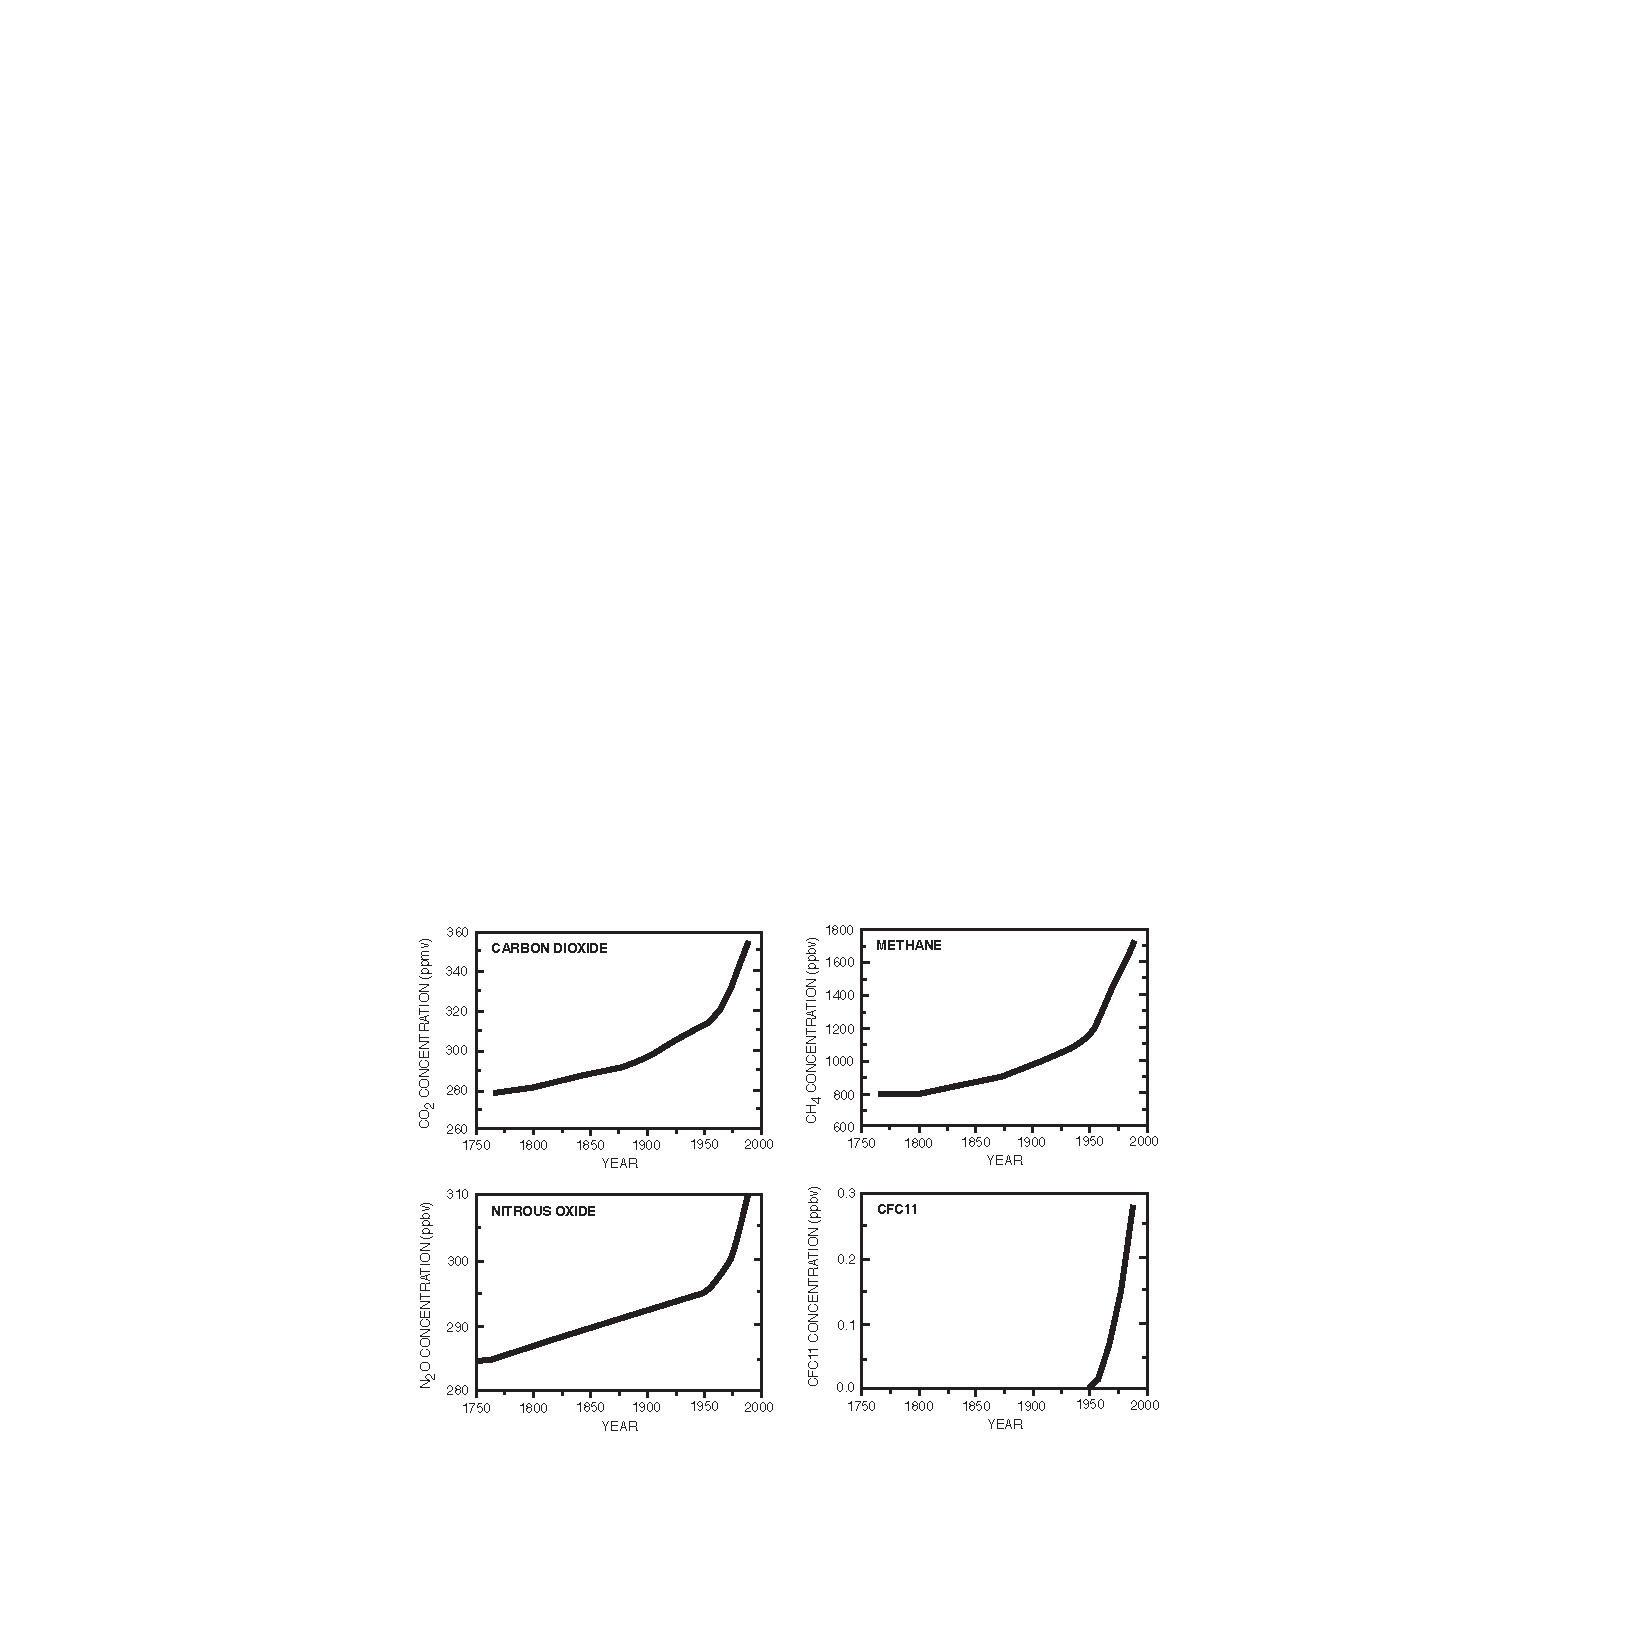
\includegraphics[width = \textwidth]{../Figures/Greenhousegases.pdf}
\caption[Concentration of greenhouse gases]{Rise in concentration of greenhouse gases since the 18th century.  Reproduced from \emph{Introduction to Atmospheric Chemistry} p. 113.\cite{Jacobs1999}}
\label{Greenhousegases}
\end{figure}

Fossil fuels are also a prominent source of chemical feedstocks.\cite{Shilov1997}  The alkanes can be converted into alkenes and alkynes \emph{via} hydrothermal cracking and these can be oxidised or otherwise converted to form useful chemical starting materials.  However, the hydrothermal cracking is highly inefficient requiring high temperatures and producing a large range of undesirable by-products.\cite{Shilov1997}  The potential environmental damage from using fossil fuels, together with the mounting costs associated with their extraction, means alternative chemical feedstocks are desirable both environmentally and economically.\cite{Poliakoff2002, Crabtree2011b}

Biogas is a mixture of gases containing primarily methane and carbon dioxide with small amounts of hydrogen sulfide, ammonia and other impurities.\cite{Abatzoglou2009}  Generated by the anaerobic digestion of wet organic waste, biogas is considered carbon neutral as the carbon in the organic matter, which is converted to the biogas, is already within the carbon cycle.\cite{Amon2007}  New Zealand has a number of plants to capture the biogas produced from landfill, sewage, farm and food waste.\cite{Biogas}  Typically the biogas collected is used for on-site electricity production or co-generation of electricity and methane.

%\begin{table}
%\caption[Biogas generation sites in New Zealand]{Biogas generation sites in New Zealand}
%\label{Biogas}
    %\begin{tabular}{l p{4cm} l l}
    %\hline
%Project name & Feedstock & Application & Year Commissioned\\ \hline
%PNCC digester upgrade & Co-digestion & Co-generation & 2008/10\\ 
%HCC Digester upgrade (Hamilton) & Co-digestion & Co-generation & projected\\ 
%Beef feedlot manure (Waikato)	& Feedlot waste & Study & 2008\\ 
%Piggery feedlot manure (Waikato)& Feedlot waste & Study & 2008\\
%Chicken Waste (Waikato)	& Industrial & Study / Research & 2008\\ 
%Tirau Dairy (Tirau) & Industrial waste & Boilers & 1990\\
%Southern Landfill, Happy Valley & Landfill & Power generation & 2008\\
%Silverstream (Lower Hutt)	& Landfill & Power generation & 1994\\
%Greenmount & Landfill & Power generation & 1992\\ 
%Rosedale & Landfill & Power generation & 1994\\
%Horotiu Landfill & Landfill & Power generation & 2004\\
%Spicer Landfill (Porirua/Wellington) & Landfill & Flaring & 2009 \\ 
%Burwood Landfill & Landfill & Co-generation & 2007\\
%Tirohia Landfill	& Landfill & Power generation & 2008\\
%Hampton Downs Landfill & Landfill & Power generation &2009\\
%Landcorp (Waimakariri/Rangiora) & Manure biosolids & Co-generation & 2007/08\\
%Kiwifruit Waste (Tauranga) & Rural waste & Study & 2008 \\
%Piggery Waste (Canterbury) & Rural waste & Study	& 2008\\ 
%Piggery Waste (Waikato)	& Rural waste & Research & 2008\\ 
%Piggery Waste (Canterbury) & Rural waste & Study & 2009\\ 
%Mangere WWTP I(Auckland) & Sewage & Co-generation	& 2004\\ 
%Hamilton WWTP (Hamilton ) & Sewage & Co-generation	& 2005\\
%Bromley WWTP & Sewage & Co-generation & 1996\\ 
%Tauranga WWTP & Sewage & Co-generation & 1996\\ 
%CCC digester upgrade (Christchurch) & Thermophilic / biosolids & Co-generation & projected\\
%GI digester (Dunedin) & Thermophilic / biosolids & Boilers & 2001\\
    %\hline
    %\end{tabular} \end{table}

Biogas also has the potential to act as a chemical feedstock for industrial processes that typically use components extracted from crude oil.\cite{Poliakoff2002}  However, there are several issues associated with the use of biogas as a chemical feedstock.  Biogas is often produced at remote sites and as it mostly contains methane, it cannot be transported economically,\cite{Crabtree2001} hence on-site conversion of the methane into a readily transportable liquid such as methanol would reduce the transportation costs considerably.  However methane, like other alkanes, is unreactive towards most chemical transformations.  Although methane can be oxidised, the low reactivity means that severe conditions or highly active reagents are required.  The methanol that is produced is more easily oxidised than methane so over-oxidation to the undesirable carbon dioxide occurs readily. \cite{Crabtree2001}  

One of the most commonly used processes to form methanol from methane is the syngas process.  This first converts the methane to carbon monoxide, then reduces it to methanol.  The formation of synthesis gas (Equation \ref{syngasequation}) is carried out over a heterogeneous nickel catalyst and requires pressures of 40 atm and high temperatures of 850 \degrees C.  This is followed by reaction over a mixture of copper, zinc oxide and alumina at 50 - 100 atm and 250 \degrees C (Equation \ref{syngasequation2}). The process is inefficient as the methane is over-oxidised before being reduced to methanol\cite{Crabtree2001} and although the production of synthesis gas yields three moles of hydrogen, only two of these are used in the production of methanol.  The addition of \ce{CO2} to the system allows for reaction of the excess hydrogen to produce methanol and water (Equation \ref{syngasequation3}).

\vspace{-1cm}
\begin{align}
\ce{CH4 + H2O} & \longrightarrow \ce{CO + 3H2} \label{syngasequation} \\[0.5cm]
\ce{CO + 2H2} & \longrightarrow \ce{CH3OH} \label{syngasequation2} \\[0.5cm]
\ce{CO2 + 3H2} & \longrightarrow \ce{CH3OH + H2O} \label{syngasequation3}
\end{align}
\vspace{-2cm}
%Green chemistry aspect\\
%CO2 harming the atmosphere\\
%Carbon cycle\\
%QC comic http://questionablecontent.net/view.php?comic=1939\\

\section{C-H activation}

Carbon-hydrogen bonds are among the least reactive bonds as evidenced by their presence in all organic molecules.\cite{Shilov1997}  Indeed the old name for alkanes ``paraffins'' is derived from the Latin \emph{parum affinis} meaning without affinity.  Alkanes have also been referred to as the ``noble gases of organic chemistry.''\cite{Shilov1997}  The carbon-hydrogen bond is considered to be a very strong bond with a bond dissociation enthalpy of 438~kJmol$^{-1}$ for methane.\cite{SI2002}  This compares to an average carbon-oxygen bond of 358~kJmol$^{-1}$, and a carbon-carbon single bond of 346~kJmol$^{-1}$.\cite{SI2002}  In addition, alkanes have very high ionisation potentials and pK\sub{a} values, and low proton affinities.\cite{Shilov2000}  Alkenes typically have stronger C-H bonds than alkanes, for example ethene and ethyne have bond dissociation enthalpies of 444 and 502 kJmol$^{-1}$ respectively, compared to 410 kJmol$^{-1}$ for ethane.\cite{Shilov1997}  However, the reduced steric hindrance in alkenes leads to greater kinetic reactivity, and stronger aryl-metal bonds result in a thermodynamic driving force for the C-H activation to occur.\cite{Crabtree2001}

%bond lengths 1.08 C-H, 1.43 C-O, 1.54 C-C

%Ethene, ethyne and benzene all have stronger C-H bonds of 444, 502 and 456 .\cite{Shilov1997}  As such, a carbon-hydrogen bond in an alkane is unlikely to react without strong reagents or severe conditions.\cite{Crabtree2001}

C-H activation refers to the increased reactivity of carbon hydrogen bonds that occurs as a result of interaction with another reagent.\cite{Crabtree2001}  Functionalisation involves the replacement of the C-H bond with another functional group (X) to form a C-X bond.  This reaction may occur in a number of different ways depending on the reactivity of the metal complex.\cite{Shilov2000}  Activation is typically easier than functionalisation as the metal alkyl and hydride often recombine \emph{via} reductive elimination during attempts to functionalise.\cite{Crabtree2001}  
%However, the functionalisation is crucial for the conversion of methane to a useful feedstock.

%The functionalisation step may be viewed as a organic reaction occuring on a metal support which is important for the activation of the bond.\fixme{reword this?}  

%This is essentially an organic reaction following activation.\cite{Crabtree2001}  

There are three main processes by which C-H activation can occur.\cite{Shilov2000}  The first is the organometallic activation which involves the formation of a metal-carbon bond.  This may involve cleavage of the bond through either oxidative addition (Equation \ref{Oxidativeequation}) or electrophilic substitution (Equation \ref{Electrophilicequation})  In the second type the alkane C-H bond interacts with a ligand on the metal rather than the metal itself (Equation \ref{Oxidationequation}).  The third type involves the generation of a reactive species by the metal complex, which then attacks the C-H bond (Equation \ref{Radicalequation}).  Systems where organometallic activation occurs will be the focus of this proposal.

\vspace{-1cm}
\begin{align}
\ce{RH + M}^{n+}	& \longrightarrow	\ce{[R-M-H]}^{n+2} \label{Oxidativeequation} \\[0.5cm]
\ce{RH + M}^{n+}	& \longrightarrow	\ce{R-M}^{(n+2)+} + \ce{H+} \label{Electrophilicequation} \\[0.5cm]
\ce{RH + O=M}^{n+} 	& \longrightarrow	\ce{R\dot} + \ce{HO-M}^{(n-1)+} \label{Oxidationequation} \\[0.5cm]
\ce{H2O2 + Fe}^{2+}	 & \longrightarrow	\ce{HO\dot{} + HO- + Fe}^{3+} \label{Radicalequation} \\
\ce{HO\dot} + \ce{RH} & \longrightarrow	\ce{H2O + R\dot} \notag \\[0.5cm]
\ce{CH4 + 2O2} & \longrightarrow \ce{CO2 + 2H2O} \label{Combustion}
\end{align}

%\fixme{similarities between C-H and H-H activation}

Alkanes can react at elevated temperature with oxygen in the atmosphere to form the thermodynamically stable products water and carbon dioxide (Equation \ref{Combustion}).  However, alkanes are inert in air at room temperature in the absence of a catalyst.\cite{Shilov1997}  Alkanes can be converted into other hydrocarbons by heating.  This forms radical species which can combine to form longer or shorter chain alkanes, alkenes and alkynes.\cite{Sironi1990}  For example, methane may be converted into ethane, ethene and ethyne by heating at temperatures in excess of 900 \degrees C.\cite{Shilov1997}  Alkanes can also be protonated by superacids, leading to elimination of hydrogen gas, giving an overall hydride abstraction reaction.  However, the elimination occurs selectively with the most basic hydride and the superacids used will attack a number of functional groups.\cite{Crabtree2004}

%\vspace{-0.8 cm}
%\begin{equation}

%\label{Combustion}
%\end{equation}

The presence of other functional groups on the molecule can result in activation of a C-H bond.  A common example of this is protons $\alpha$ to a carbonyl group that are easily removed in the presence of a base.  This forms the basis for a number of widely utilised organic reactions such as the aldol condensation reaction (Scheme~\ref{Aldolcondensation})\cite{Saito2004}.  However in alkanes, no functional groups are present to activate the bond so it is necessary to activate the bond using an external source such as an enzyme or coordination complex.\cite{Crabtree2001}

\begin{scheme}[h]  
  \centering
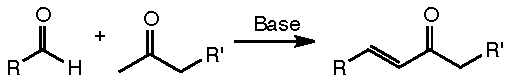
\includegraphics[]{../Schemes/Aldolcondensation.pdf}
 \caption[Aldol condensation reaction]{Aldol condensation reaction}
 \label{Aldolcondensation}
\end{scheme}

%104 kcal mol-1 = ~435 kJmol-1

Complex organic molecules are synthetic targets as a result of their potential use as pharmaceuticals.  Currently the synthesis of these target molecules relies on the modification of existing functional groups.  The regio- and stereo-selective activation and functionalisation of C-H bonds within complex organic molecules would result in a major paradigm shift in organic synthesis.\cite{Davies2008}

\subsection{Biological systems}

As previously discussed, the oxidation of methane to methanol without over-oxidation to carbon dioxide is desirable in order to make use of biogas as a chemical feedstock.\cite{Crabtree2001}  Like many other desirable chemical transformations, enzymes exist that are capable of performing the reaction.  Methane monooxygenase and cytochrome P450 catalyse the oxidation of alkanes to alcohols (Equation \ref{Methanemonooxygenaseequation}).\cite{Crabtree1995}  Although methane monooxygenase is specfic for methane, cytochrome P450 enzymes will catalyse the oxidation of a range of alkanes.\cite{Lipscomb1994, Crabtree2001}

\vspace{-0.8 cm}
\begin{equation}
\ce{NADPH + O2 + RH + H+} \longrightarrow \ce{NADP+ + H2O + ROH}
\label{Methanemonooxygenaseequation}
\end{equation}

Methane monooxygenase is found in bacteria that exist at the interface of aerobic and anaerobic environments found in lakes, oceans and soils.\cite{Lipscomb1994}  These bacteria are described as methanotrophic, they utilise methane as their source of carbon and energy.\cite{Haber1983}  Methane monooxygenase consists of three proteins; component B, reductase and hydroxylase.\cite{Lipscomb1994}  The hydroxylase protein contains a dinuclear iron centre that activates oxygen to form an oxo-bridged system.  This reacts with methane to give methanol and a hydroxo-bridged diiron centre.\cite{Merkx2001}  However, despite numerous studies,\cite{Lipscomb1994, Merkx2001, Tinberg2011} the mechanism of methane monooxygenase has proved elusive with a number of different mechanisms proposed (Scheme \ref{Methanemonooxygenasemechanism}).

%The hydroxylase protein contains a hydroxo-bridged dinuclear iron that forms that active catalytic site.  Both iron atoms are reduced to Fe(II) and then react with \ce{O2} The O-O bond is cleaved to give water and a Fe(IV)Fe(IV)=O species which can abstract a hydrogen from methane.  This gives an OH radical and a \ce{CH3} radical which recombine to form methanol.\fixme{SCHEME}

%\begin{figure}[h]
%\centering
%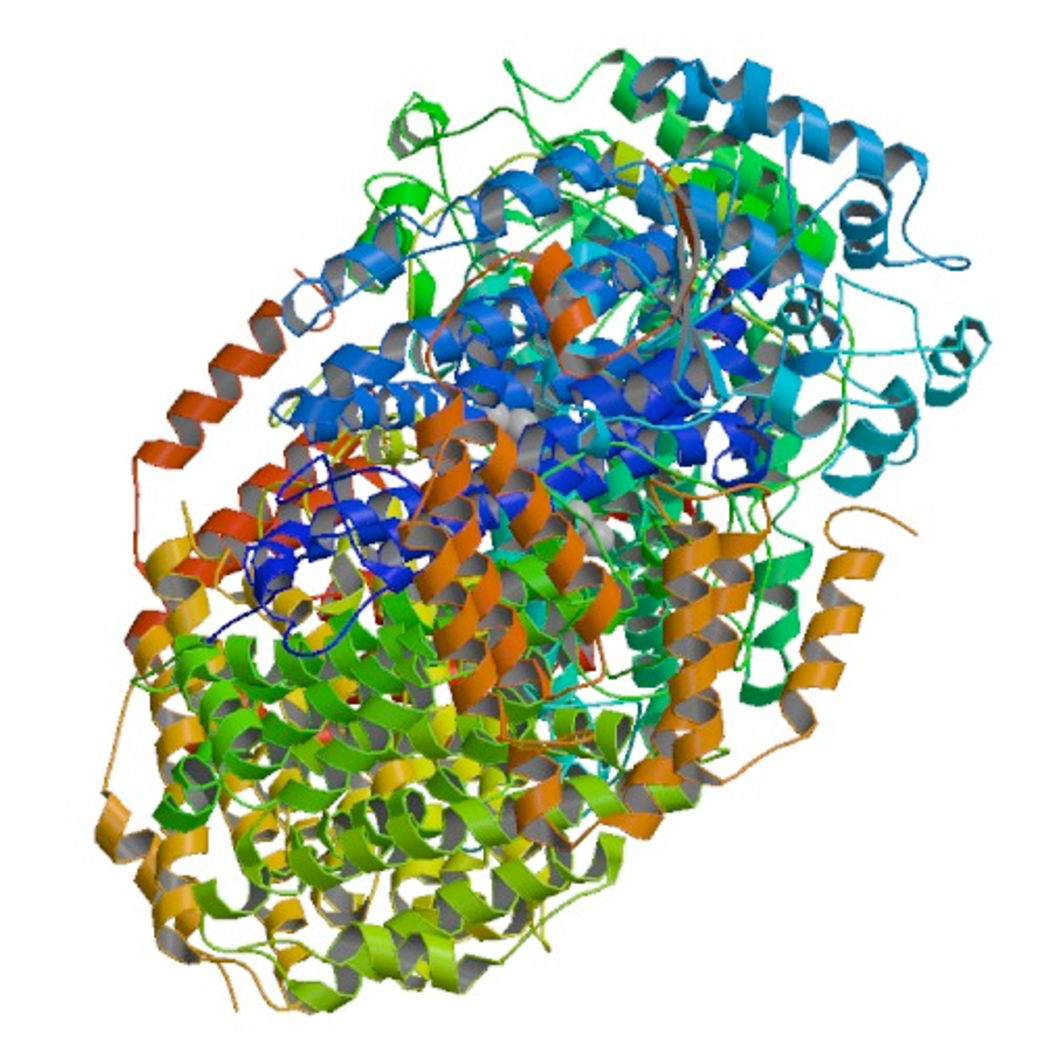
\includegraphics[height = 5cm]{../Figures/Methanemonooxygenase.pdf}
%\caption[X-ray crystal structure of methane monooxygenase]{X-ray crystal structure of methane monooxygenase reproduced from \fixme{reference from protein databank}}
%\label{Methanemonooxygenase}
%\end{figure}

\begin{scheme}[h]
\centering
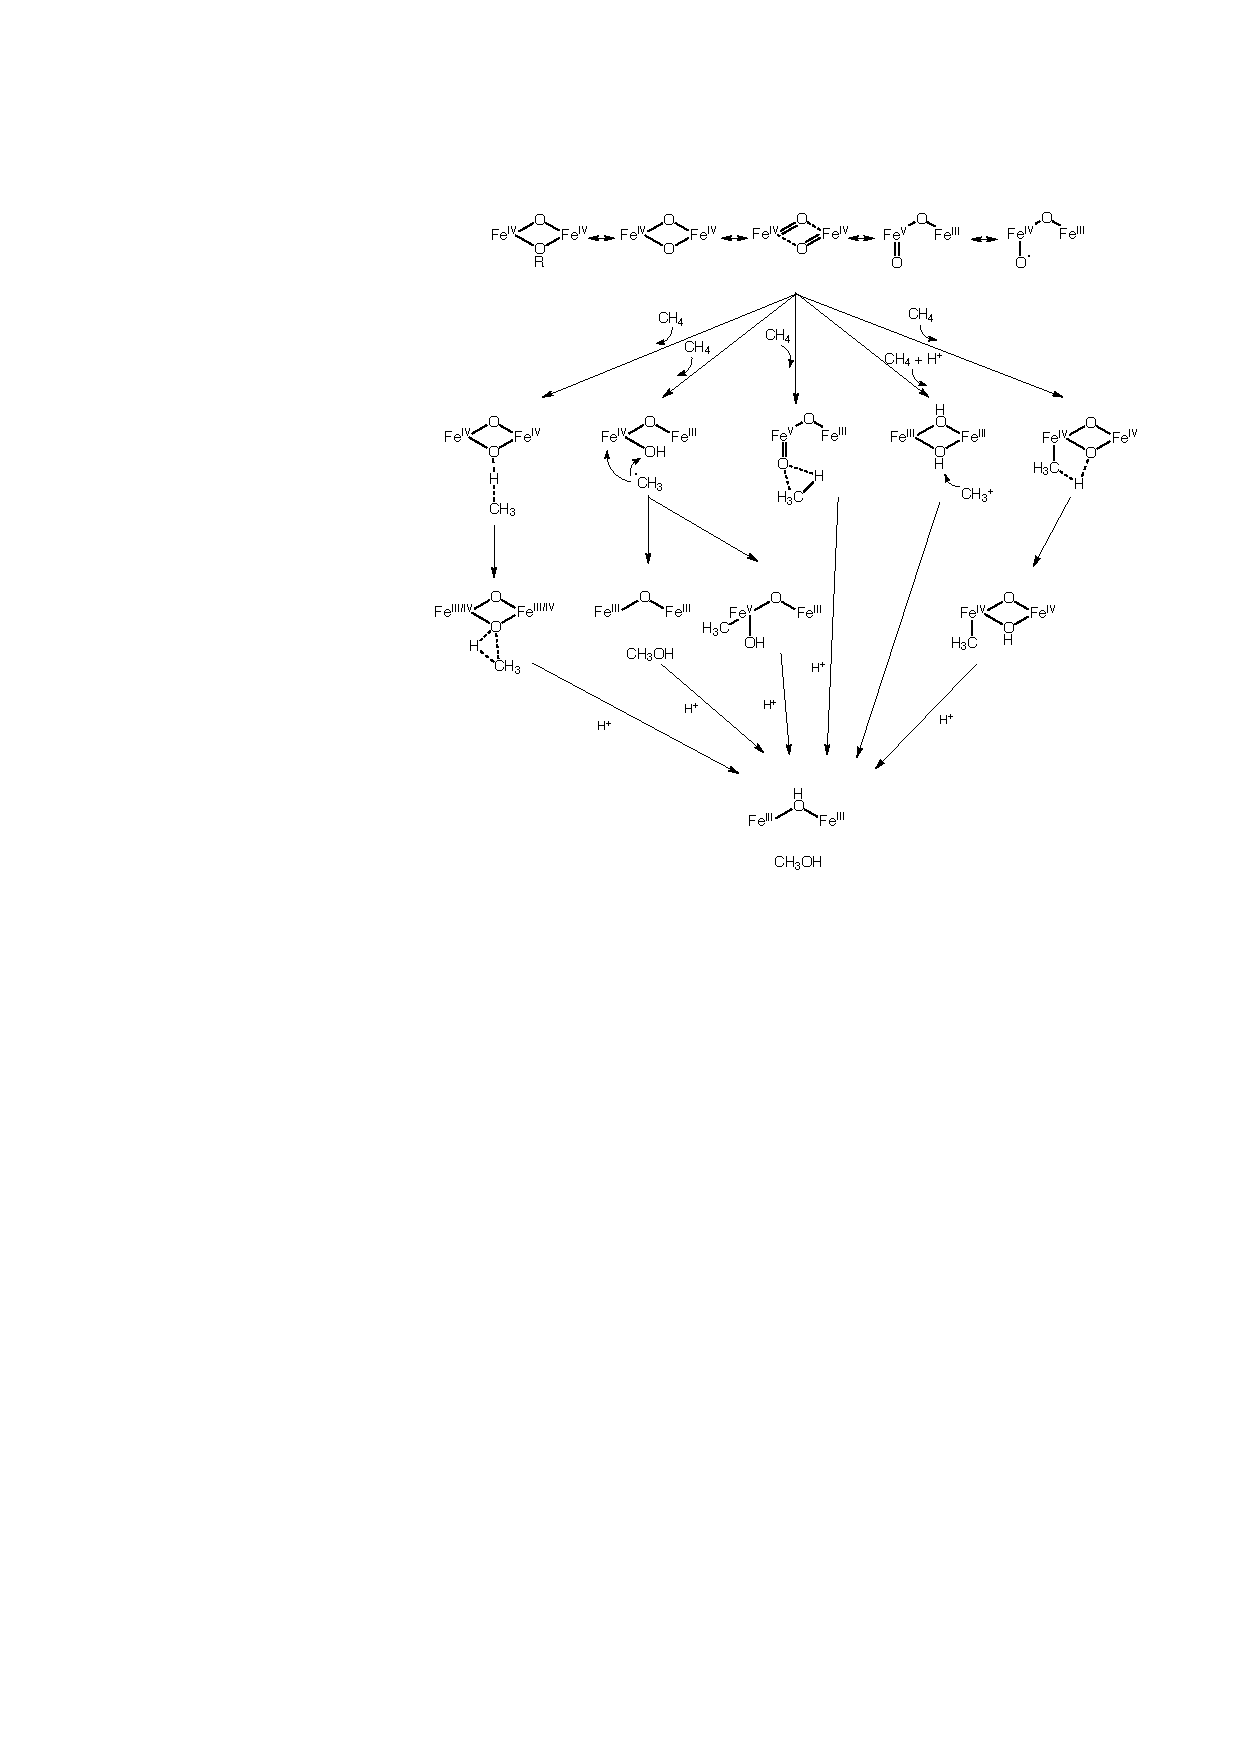
\includegraphics[width = 0.95\textwidth]{../Schemes/Methanemonooxygenasemechanism.pdf}
\caption[Proposed mechanisms for the hydroxylation of methane]{Proposed mechanisms for the hydroxylation of methane reproduced from Lippard et al.\cite{Merkx2001}}
\label{Methanemonooxygenasemechanism}
\end{scheme}

Cytochrome P450 enzymes are found in a most classes of organisms including bacteria, fungi, plants, insects and mammals.\cite{Montellano2010}  The consistent feature across all P450 enzymes is the presence of a heme group with a coordinated thiolate ion at the active site of the molecule.\cite{Montellano2010}  The first step in metabolism of pharmaceuticals in the body, phase 1, typically involves oxidation, reduction and hydrolysis reactions.  P450 enzymes are responsible for the phase 1 metabolism of around 75\% of known pharmaceuticals.\cite{Rittle2010}  Although the enzymes perform a number of roles, one of the most interesting is the hydroxylation of C-H bonds.\cite{Rittle2010}

The overall catalytic cycle for the hydroxylation of an alkane by a P450 enzyme reported by de Montellano\cite{Montellano2010} is given in Scheme \ref{P450catalyticcycle}.  In the resting state (A) the Fe(III) is bound to a thiolate and the \emph{trans} ligand is typically a water molecule though some P450's do not have a \emph{trans} ligand.  The water is displaced upon binding of an RH group.  Binding of the RH allows electron transfer to occur, reducing the Fe(III) to Fe(II) (C).  Oxygen binds to the Fe(II) resulting in the superoxide complex D.  This undergoes electron transfer and protonation to form the hydroperoxo complex E.  This complex is protonated and undergoes loss of \ce{H2O} to form the porphyrin radical cation F.  F can then react with the substrate to give the alcohol product.  Following product release and rebinding of water the resting state is restored.

%\begin{figure}[h]
%\centering
%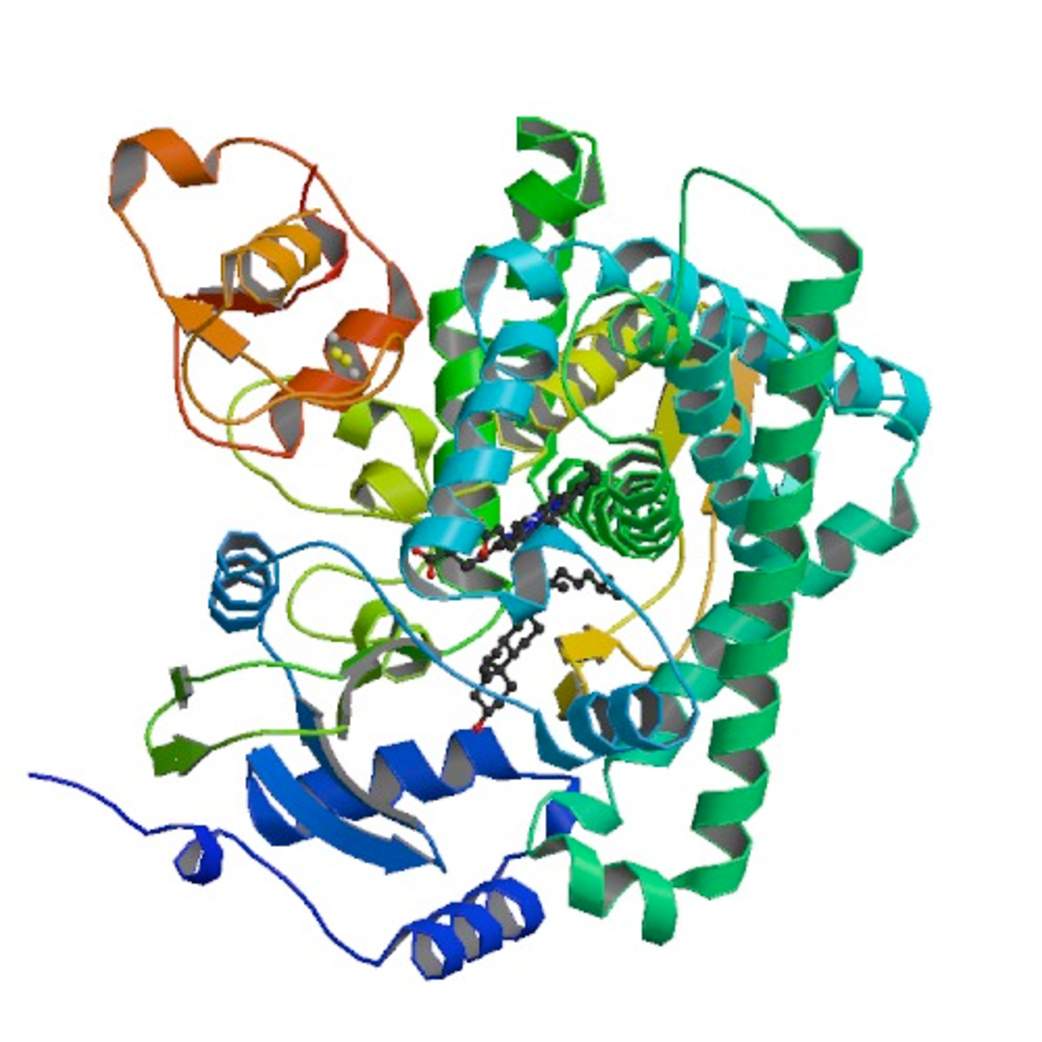
\includegraphics[height = 5cm]{../Figures/P450.pdf}
%\caption[X-ray crystal structure of P450]{X-ray crystal structure of P450 reproduced from \fixme{reference from protein databank}}
%\label{P450}
%\end{figure}

\begin{scheme}[h]
\centering
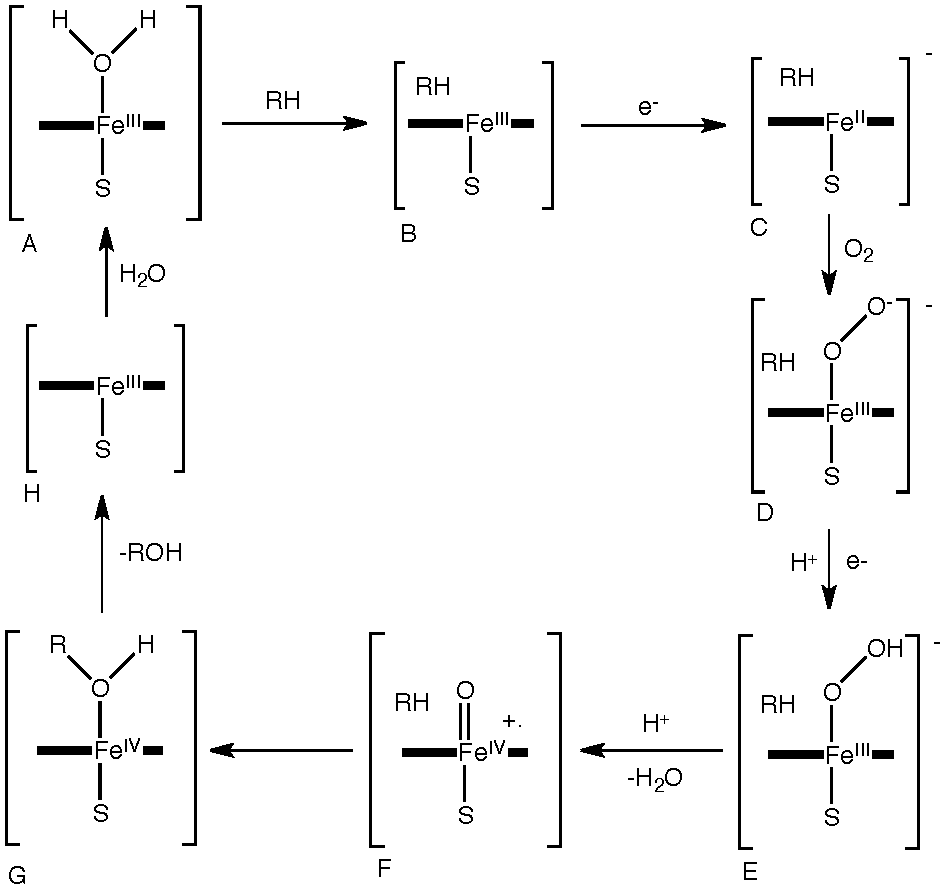
\includegraphics[width = 0.75\textwidth]{../Schemes/P450catalyticcycle.pdf}
\caption[Proposed catalytic cycle for hydroxylation by P450]{Proposed catalytic cycle for hydroxylation by P450 reported by de Montellano\cite{Montellano2010}}
\label{P450catalyticcycle}
\end{scheme}

\subsection{Organometallic systems}

There are a number of different types of bonds that can form in organometallic systems (Figure \ref{Bondingmodes}).  The most common is the donation of a ligand lone pair of electrons to a vacant orbital on the metal (a).  This is typically observed for ligands such as \ce{PR3,~CH3^-~and~H2O} among many others.  Donation of a $\pi$-bonding pair of electrons to the metal (b) is also common, typically among the alkene complexes such as those with ethene.  There are a number of rarer bonding forms including the donation of a $\sigma$-bonding pair of electrons (c) and the alkyl agostic interaction (d).\cite{Bernskoetter2009}  In addition, the metal can donate electron density from filled d orbitals into the LUMO of the ligand (either the $\sigma$* or $\pi$* orbital).\cite{Chatt1955}

\begin{figure}[h]
\centering
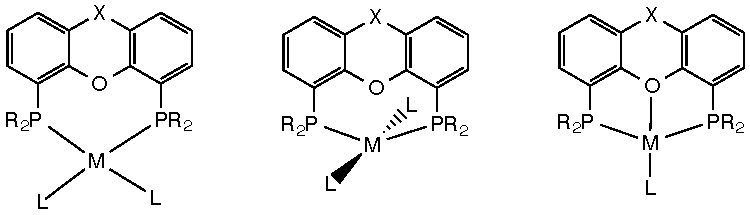
\includegraphics[width = 0.5\textwidth]{../Figures/Bondingmodes.pdf}
\caption[Bonding in organometallic complexes]{Bonding in organometallic complexes}
\label{Bondingmodes}
\end{figure}

Alkanes are weak $\sigma$-bases and $\pi$-acids.  As such they are very poor ligands for transition metals.\cite{Crabtree1993}  Typically alkanes form $\sigma$-complexes with metals that can $\pi$-backbond.  For successful complexation a low valent metal and the absence of competitive decomposition pathways are required.\cite{Crabtree2001}  Enhanced bonding of alkanes occurs with metals capable of forming enhanced $\pi$-backbonding into the $\sigma$* C-H orbital, similar to that found for molecular hydrogen complexes.\cite{Kubas1988}

The activation of C-H bonds is thought occur \emph{via} a stepwise process involving the coordination of the alkane to the metal to form a $\sigma$-complex, followed by the oxidative cleavage of the C-H bond forming metal-alkyl and metal-hydride bonds.\cite{Labinger2002}  The intermediate  $\sigma$-complexes are highly unstable and until recently their existence had only been inferred by isotope scrambling and the inverse kinetic isotope effect in reductive elimination reactions of alkyl hydrides.\cite{Bernskoetter2009, Labinger2002}  In 2009 Brookhart reported the characterisation of a relatively long-lived rhodium(I) $\sigma$-methane complex.\cite{Bernskoetter2009}  The complex was formed by the protonation of a rhodium methyl complex (Scheme \ref{Sigmamethane}).  At -87~\degrees C the methane is displaced by solvent (\ce{CDCl2F}) with a half-life of 83 minutes.

\begin{scheme}[h]
\centering
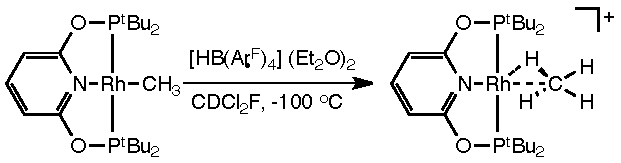
\includegraphics[]{../Schemes/Sigmamethane.pdf}
\caption[Formation of a $\sigma$-methane complex]{Formation of a $\sigma$-methane complex.  Ar\ce{^{F}} = \emph{m}-di(trifluoromethyl)phenyl}
\label{Sigmamethane}
\end{scheme}

%$\sigma$-Complexes of methane have been proposed 
%The first example of C-H activation was reported by Dimroth in 1902\cite{Dimroth1902}  Reaction of phenol with a solution of mercury acetate on a steam bath replaced the \emph{ortho} and \emph{para}-protons with a mercury acetate group.  \fixme{more info etc}

C-H activation has developed significantly since the first example of C-H activation by an organometallic complex was reported by Chatt in 1962. \cite{Chatt1962}  Reduction of metal halides by sodium napthalene in the presence of an excess of \gls{dmpe} produced V, Cr, Mo and W complexes of the form \ce{[M(}\gls{dmpe}\ce{)_3]},  and Fe and Co complexes of the form \ce{[M(}\gls{dmpe}\ce{)_2]}.  However, the \ce{[Ru(}\gls{dmpe}\ce{)_2]} analogue gave a hydride complex ``by taking hydrogen from the napthalene.''\cite{Chatt1962}  

Further analysis of the ruthenium system was carried out and published in 1965.\cite{Chatt1965} Reaction of \emph{cis}- or \emph{trans}-\ce{[RuCl2(}\gls{dmpe}\ce{)_2]} with benzene, naphthalene, anthracene and phenylanthracene formed the \emph{cis}-\ce{[RuH(aryl)(}\gls{dmpe}\ce{)_2]} (aryl = phenyl, naphthyl, anthryl and phenanthryl) complexes \emph{via} oxidative addition.\cite{Chatt1965}  The activation is reversible, as reactions of the complexes with hydrochloric acid yielded hydrogen gas, the aromatic starting material and \emph{cis}-\ce{[RuCl2(}\gls{dmpe}\ce{)_2]} (Equation \ref{ChattCH}).  The C-H activation to form the complexes was selective for example, in the reaction with naphthalene the activation occurred exclusively at the 2-position.

\vspace{-0.6 cm}
\begin{equation}
\ce{[RuH(C10H7)(dmpe)2] + 2HCl} \longrightarrow \ce{[RuCl2(dmpe)2] + H2 + C10H8}
\label{ChattCH}
\end{equation}

The naphthyl hydride complex formed by treatment of \ce{[Ru(}\gls{dmpe}\ce{)_2]} with naphthalene thermally decomposed giving a complex with properties consistent with \ce{[Ru(}\gls{dmpe}\ce{)_2]} (Scheme \ref{Chattdmpescheme}).\cite{Chatt1965}  However, infrared spectroscopy showed a signal for a Ru-H at 1791 \percm,  leading to the proposed structure of \ce{[RuH(CH2PMeCH2CH2PMe2)(}\gls{dmpe})], formed by activation of a C-H bond from the \gls{dmpe} ligand.\cite{Chatt1965}  X-ray crystallography later allowed the reformulation of the structure to the analogous dimer.\cite{Crabtree2004}  However, this species remains the first example of cyclometallation of an sp$^3$ C-H bond.

\begin{scheme}[h]
\centering
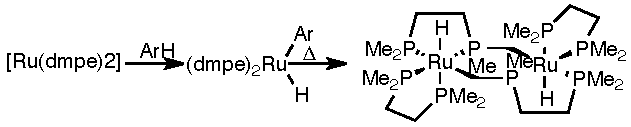
\includegraphics[]{../Schemes/Chattdmpescheme.pdf}
\caption[C-H activation reactions reported by Chatt and Davidson]{C-H activation reactions reported by Chatt and Davidson\cite{Chatt1965}}
\label{Chattdmpescheme}
\end{scheme}

The exchange of hydrogen with deuterium in polyalkyl benzenes, polycyclic aromatic hydrocarbons and heterocycles can be catalysed by homogeneous platinum (II) species.\cite{Hodges1968, Hodges1969, Hodges1969b}  Using deutero-acetic acid as a solution in \ce{D2O}, together with DCl or anhydrous tin(IV) chloride to prevent the formation of platinum metal, H/D exchange on the substrate was observed when exposed to \ce{Na2PtCl4} or \ce{K2PtCl4}.\cite{Hodges1968, Hodges1969}  Although the rate of exchange was faster for unhindered aromatic protons, H/D exchange was also observed for alkyl protons.\cite{Hodges1969b}  The rate was fastest for \hbox{\emph{p}-xylene}, \gls{mesitylene}, \emph{m}-xylene and toluene, however exchange of alkyl protons was also observed in \emph{o}-xylene, \gls{hemimellitene} and \gls{durene}.\cite{Hodges1969b}

This activation of alkyl protons inspired Shilov to investigate the C-H activation of alkanes by platinum.  The system carries out oxidation of alkanes such as methane \emph{via} electrophilic activation (Scheme \ref{Shilovcatalyticcycle}).\cite{Labinger2002, Crabtree2001}  The first step involves displacement of a chloride ligand on the platinum by a $\sigma$-methyl followed by oxidative addition and loss  of H$^+$ \emph{via} loss of HCl.  The Pt(II) is then  oxidised to Pt(IV) \emph{via} electron transfer to the \ce{PtCl6}$^{2-}$.  Finally, the complexed methyl undergoes nucleophilic attack from water displacing the \emph{trans} chloride ion to form HCl, methanol and regenerate the catalyst.  The system has shown selectivity for terminal C-H bonds.  For example, in the oxidation of ethanol functionalisation occurs at the methyl to yield ethylene glycol (Equation \ref{Ethyleneglycol}) whilst, all other methods of oxidation will oxidise the hydroxyl functionality.\cite{Labinger1993}  This can be utilised for the one-pot synthesis of ethylene glycol from ethanol.\cite{Sen1994}  However, the selectivity is lost in reaction with 2-propanol which gives only acetone.\cite{Labinger1993}
\vspace{-1.5cm}
\begin{scheme}[h]
\centering
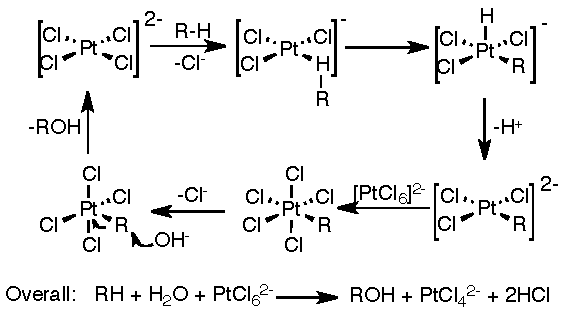
\includegraphics[]{../Schemes/Shilovcatalyticcycle.pdf}
\caption[Platinum catalysed oxidation of alkanes]{Platinum catalysed oxidation of alkanes}
\label{Shilovcatalyticcycle}
\end{scheme}

\begin{equation}
\ce{CH3CH2OH + H2O + PtCl6}^{2-} \longrightarrow \ce{CH2OHCH2OH + PtCl4}^{2-} + \ce{2HCl} 
\label{Ethyleneglycol}
\end{equation}

Although the Shilov system is catalytic in Pt(II), it requires a stoichiometric amount of Pt(IV).  In addition, the Pt(II) catalyst is unstable in solution and eventually precipitates as platinum metal.\cite{Luinstra1995}  This results in an expensive and thus impractical system for industrial application.  The relatively low yields of the system also reduce its industrial viability.\cite{Periana1993}  Furthermore, the reaction produces two equivalents of hydrochloric acid which require disposal at significant cost.\cite{Poliakoff2001}  A number of attempts have been made to replace the Pt(IV) primary oxidant thus making an economically viable system.\cite{Periana1993, Periana1998, Hashiguchi2010}  However, this has proven challenging as most oxidants tend to convert Pt(II) to the inactive Pt(IV).\cite{Crabtree2001}  Additionally, an oxidant is required that will not attack the product alcohol.  

In 1993 Periana reported the use of concentrated sulfuric acid as the primary oxidant and Hg(II) as a catalyst in place of the platinum.\cite{Periana1993}  The Hg(II) is the highest possible oxidation state so further unwanted oxidation of the catalyst is not possible.  Using methane as the feedstock, the system produces methyl bisulfate in a 43\% yield (Scheme \ref{Mercurycatalyticcycle}).  This has the advantage of being highly resistant to oxidation preventing the formation of carbon dioxide. However, the catalysis involves the formation of MeHg(II)$^+$ as an intermediate following activation.  Methyl mercury salts, like most organomercury compounds, are extremely toxic and exhibit accumulation effects in biological systems.\cite{MethylmercuryMSDS}  Sulfur dioxide, a significant contributor to acid rain,\cite{Jacobs1999} is also produced as a stoichiometric byproduct of this reaction.  However, the oxidation of sulfur dioxide to sulfuric acid by air is an established industrial process and could be utilised to provide further sulfuric acid for the process.\cite{Periana1993}

%\begin{equation}
%\ce{CH4 + 2H2SO4} \longrightarrow \ce{CH3OSO3H + 2H2O + SO2} 
%\label{Mercuryequation}
%\end{equation}

%Periana 1993 reaction is carried out at 180 degrees
%Periana 1998 reaction is carried out at 100 degrees

\begin{scheme}[h]
\centering
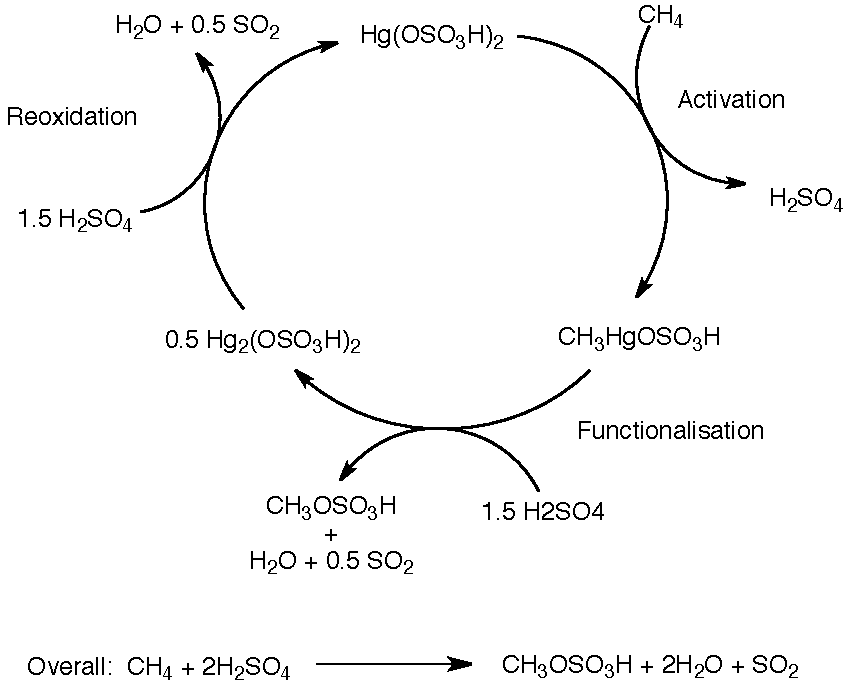
\includegraphics[width = 0.8\textwidth]{../Schemes/Mercurycatalyticcycle.pdf}
\caption[Mercury catalysed oxidation of methane]{Mercury catalysed oxidation of methane}
\label{Mercurycatalyticcycle}
\end{scheme}

Further work by Periana investigated changing the Pt(II) system to improve stability, activity and prevent oxidation to Pt(IV).\cite{Periana1998}  Nitrogen donor ligands were utilised as oxygen systems have high kinetic lability on platinum and phosphorus ligands have poor oxidative and thermal stability.  The use of \emph{cis}- or \emph{trans}-\ce{[PtCl2(NH3)2]} in concentrated sulfuric acid at 180~\degrees C gave 90\% selectivity for methyl bisulfate.  However, the catalyst degraded to insoluble \ce{PtCl2} and \ce{NH4HSO4}.  

In an extension of this work a $\pi$-acidic chelating donor ligand \gls{bpym} was utilised as $\pi$-donor ligands were expected to have lower proton affinity and form stronger Pt-N bonds than the \ce{NH3} ligands used previously.  The \ce{[PtCl2(}\gls{bpym})] complex was tested in 20 \% \ce{SO3} in \ce{H2SO4} at 200~\degrees C for 50 hours.  Some free ligand and HCl was observed, however the solution remained homogenous showing no formation of platinum metal or other insoluble products.  Using \emph{cis}-\ce{[PtCl2(}\gls{bpym})] in the catalytic system at 220~\degrees C for 2.5 hours resulted in 90\% methane conversion with an 81\% selectivity (carbon dioxide forming the major byproduct).\cite{Periana1998}  However, this reaction requires high temperatures and forms significant amounts of carbon dioxide and sulfur dioxide both of which are environmentally hazardous.\cite{Jacobs1999}  The reaction proceeds \emph{via} a slightly different mechanism to the mercury system (Scheme \ref{PerianaPtcycle}) with oxidation occurring prior to the functionalisation.\cite{Periana1998}

%\begin{figure}[h]
%\centering
%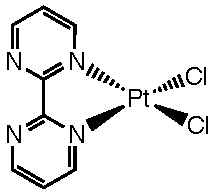
\includegraphics[height = 4cm]{../Figures/bpym.pdf}
%\caption[Structure of \ce{[PtCl2(bpym)]}]{Structure of \ce{[PtCl2(bpym)]}}
%\label{bpym}
%\end{figure}

\begin{scheme}[h]
\centering
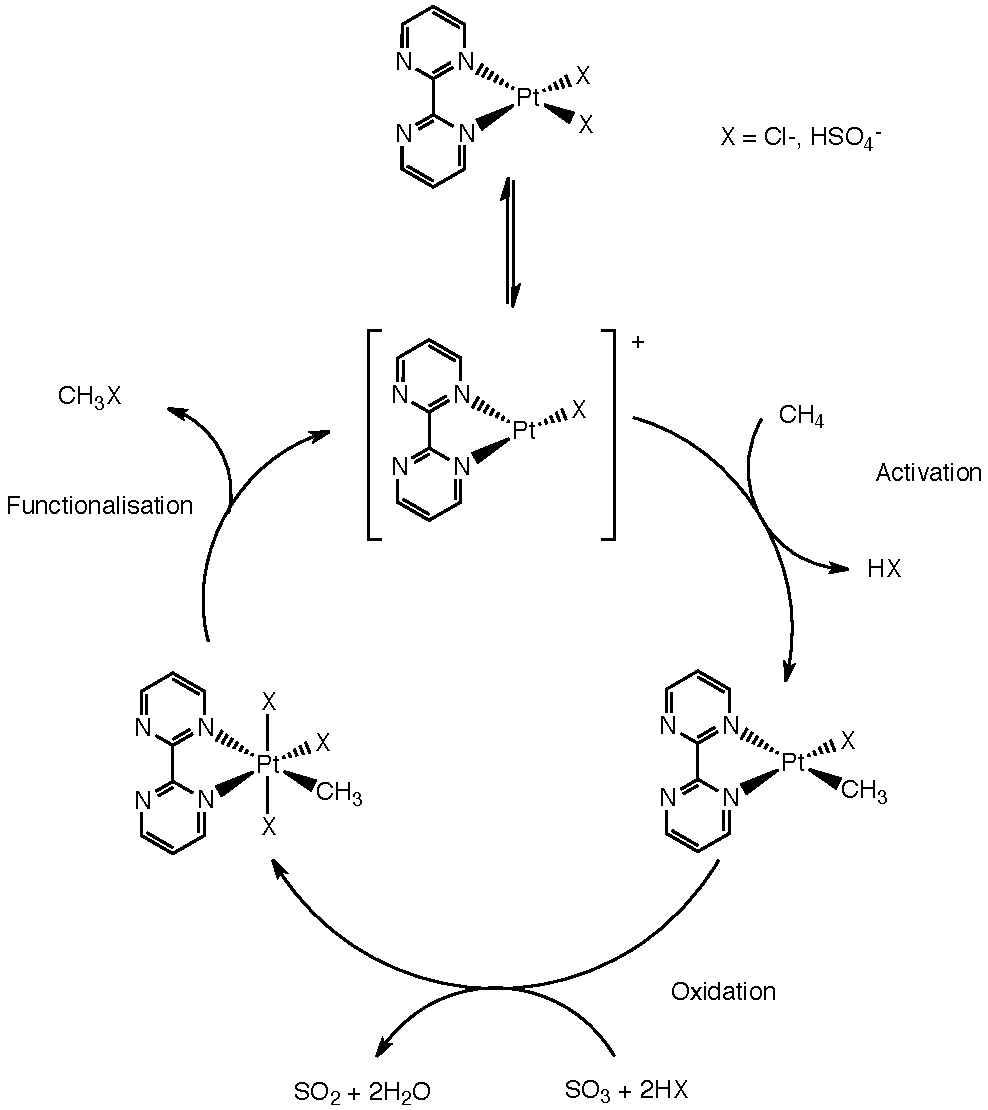
\includegraphics[width = 0.9\textwidth]{../Schemes/PerianaPtcycle.pdf}
\caption[Oxidation of methane catalysed by \ce{[PtCl2(bpym)]}]{Oxidation of methane catalysed by \ce{[PtCl2(bpym)]}}
\label{PerianaPtcycle}
\end{scheme}

%Nature of the C-H bond\\ 
%Strong\\
%Highly non-polar\\
%General catalytic attempts\\
%Shilov etc.\\

\subsection{Alkane dehydrogenation}

Alkane dehydrogenation is an alternative approach that combines the activation and functionalisation into a single step.  This methodology was developed from the \hbox{organometallic} complexes such as Wilkinson's\cite{Osborn1966} and Crabtree's\cite{Crabtree1979b} catalysts (Figure \ref{Wilkinsoncrabtree}) that are utilised as homogeneous hydrogenation catalysts.  Wilkinson's catalyst was the first homogeneous hydrogenation catalyst with comparable rates to the heterogeneous counterparts and has become very widely utilised in organic synthesis.\cite{Knowles2003}

\begin{figure}[h]
\centering
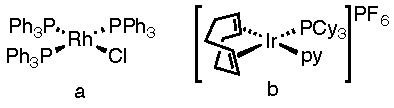
\includegraphics[]{../Figures/Wilkinsoncrabtree.pdf}
\caption[Wilkinson's and Crabtree's catalysts]{Wilkinson's (a) and Crabtree's (b) catalysts}
\label{Wilkinsoncrabtree}
\end{figure}

Crabtree reported a number of hydrogenation catalysts based on Wilkinson's catalyst in 1977.\cite{Crabtree1977} The most active of these, \ce{[Ir(cod)(PCy3)(py)]PF6} (Figure \ref{Wilkinsoncrabtree} b, \gls{cod} = 1,5-cyclooctadiene, \gls{Cy}~=~cyclohexyl, \gls{py} = pyridyl) has become known as Crabtree's catalyst.\cite{Cui2005}  This catalyst is active for the hydrogenation of a range of \hbox{mono-,} di-, \hbox{tri-,} and \hbox{tetra-substituted} alkenes with turnover frequencies (\glspl{TOF}) of 6400, 4500, 3800 and 4000 for hex-1-ene, cyclohexene, 1-methylcyclohexene and 2,3-dimethylbut-2-ene respectively.\cite{Crabtree1979b}  Crabtree's catalyst is useful for the hydrogenation of tri- and tetra-substituted alkenes for which Wilkinson's catalyst is inactive.\cite{Cui2005}

A catalytic system lowers the activation energy for a reaction, hence both the forward and reverse reactions will be catalysed.\cite{Crabtree2001}  This realisation led Crabtree to test an iridium system for dehydrogenation of alkenes.\cite{Crabtree1979}  The dehydrogenation would normally be strongly endothermic so the substrates were chosen to give products that would bind strongly to the metal to improve the thermodynamics of the reaction.  In the presence of \ce{[IrH2(alkene)2(PPh3)2]+} and 3,3-dimethylbut-1-ene (as hydrogen acceptor) the dehydrogenation of cyclooctene, [2.2.2]bicyclooctene, cyclopentene and cyclohexene were carried out successfully to give complexes of the type \ce{[Ir(diene)(PPh3)2]+} and \ce{[Ir(Cp)H(PPh3)]+} (Cp = cyclopentadienyl).\cite{Crabtree1979}  The dehydrogenation of alkanes was also possible with the system.  The dehydrogenation of cyclopentane to form the cyclopentadienyl complex gave a 30\% yield after 18 hours, whilst the dehydrogenation of cyclooctane to the cyclooctadiene complex gave a 70\% yield after only 4 hours.\cite{Crabtree1979}

Felkin reported a rhenium complex capable of dehydrogenating linear alkanes to dienes.\cite{Baudry1982}  In the presence of \ce{[ReH7(PAr3)2]} (Ar = \emph{p}-\ce{MeC6H4}) and 3,3-dimethylbut-1-ene, \emph{n}-pentane was dehydrogenated to form a diene complex (Scheme \ref{Pentanedehydrogenation}).  Treatment of this complex with \ce{P(OMe)3} produced pent-1-ene with a yield of 45\%.  This was extended to the linear isomers of hexane, heptane and octane.\cite{Baudry1984}  Although pentane can form only one conjugated diene complex, hexane and heptane can give two, whilst octane can give three.  However, in all cases upon treatment of the complex with \ce{P(OMe)3} the terminal alkene was formed with a selectivity of over 95\%.\cite{Baudry1984}  

\begin{scheme}[h]
\centering
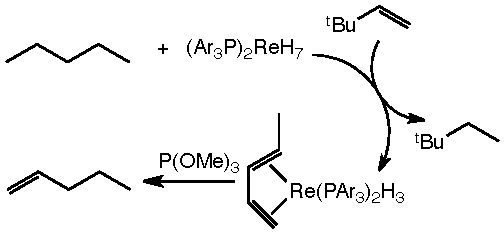
\includegraphics[]{../Schemes/Pentanedehydrogenation.pdf}
\caption[Dehydrogenation of pentane]{Dehydrogenation of pentane reproduced from Felkin et al.\cite{Baudry1982}}
\label{Pentanedehydrogenation}
\end{scheme}

Wilkinson's catalyst (figure \ref{Wilkinsoncrabtree}b) has also been utilised as a dehydrogenation catalyst.\cite{Fujii1990}  The dehydrogenation of cyclooctane to give cyclooctene by \ce{[RhCl(L)3]} (L = \ce{PPh3} or P(\emph{p}-\ce{tolyl)3}) was carried out at reflux (151~\degrees C) without the need for a hydrogen acceptor.  The high temperature of the reaction mixture is sufficient to allow the removal of molecular hydrogen from the reaction mixture.\cite{Fujii1990}  The reaction rates obtained with this system were low, the highest with L = P(\emph{p}-\ce{tolyl)3} was only 1.24 h\ce{^{-1}} with a L/Rh ratio of 8.\cite{Fujii1990}

Crabtree utilised this acceptorless methodology to test the catalytic activity of iridium complexes.\cite{Aoki1993}  \ce{[IrH2L(PCy3)2]} (L = \ce{O2CCF3}, \ce{O2CC2F5} and \ce{O2CPhCH2}) were active for the dehydrogenation of cyclooctane under reflux with initial turnover frequencies of 1.41, 1.05 and 0.22 \ce{h^{-1}} respectively.  However, the complexes were unstable with deactivation half lives of 15, 34 and 14 hours respectively.\cite{Aoki1993}  Alternate methods to remove the hydrogen were also tested.  Using perfluorodecalin as a solvent allowed for more effective hydrogen removal due to the higher volatility compared to cyclooctane.  This resulted in poor activity with a turnover frequency of 0.24 \ce{h^{-1}} using \ce{[IrH2(O2CCF3)(PCy3)2]} as catalyst.  Bubbling inert gas was unsuccessful with cyclooctane as a substrate as a large amount of the substrate was lost.  However, using the less volatile cyclodecane a turnover frequency of 0.48 \ce{h^{-1}}  was obtained.\cite{Aoki1993}

%\fixme{Goldman reference 4 from Gupta1996 had an improved non-pincer system}

\section{Pincer ligands}

Recently, the so-called pincer ligands have attracted a great deal of research attention due to their unique balance of stability and reactivity.\cite{Becerra2009}  Pincer ligands are tridentate ligands that bind in a meridional fashion, examples of which are given in Figure \ref{Pincernaming}.  Pincer ligands are named based on their donor atoms such as, PCP, NCN, and POP.  If the groups between the donor atoms contain heteroatoms then these may be included in the naming also, for example POCOP.  The pincer ligands may be anionic (as with PCP ligands) or neutral (PNP and POP).\cite{Vlugt2009, Kataoka1995}  Although phosphines are the most common donor groups, amines,\cite{Singleton2003} imines,\cite{Takenaka2005} thioethers\cite{Zim2000} and N-heterocyclic carbenes\cite{Hahn2007} have all been reported.

\begin{figure}[h]
\centering
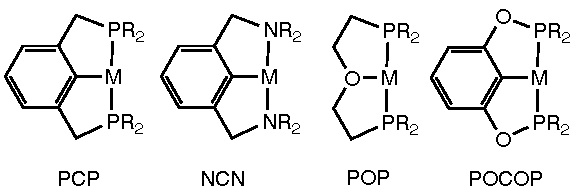
\includegraphics[]{../Figures/Pincernaming.pdf}
\caption[Naming of pincer ligands]{Naming of pincer ligands}
\label{Pincernaming}
\end{figure}

The first reports of pincer ligands were in 1976 by Shaw\cite{Moulton1976} and Alcock.\cite{Alcock1976}  Shaw reported a \emph{tert}-butyl PCP ligand (Figure \ref{Shaw}) and introduced the naming scheme that has become commonplace for pincer ligands.  When reacted with an appropriate metal precursor, complexes formed between the tridentate ligand with nickel, palladium, platinum, rhodium and iridium with chloride, nitrile, hydride and carbon monoxide ligands.\cite{Moulton1976} 

\begin{figure}[h]
\centering
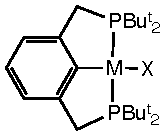
\includegraphics[]{../Figures/Shaw.pdf}
\caption[First reported PCP pincer ligand]{First reported PCP pincer ligand}
\label{Shaw}
\end{figure}

Alcock reported X-ray crystal structures of the first complexes of POP ligands (Figure \ref{Alcock}).\cite{Alcock1976}  These formed rhodium carbonyl complexes that were characterised by X-ray crystallography.  With a single ether group in the backbone it forms a typical pincer complex, bonding through the phosphorus and oxygen atoms.  However, when there are three ether units the phosphorus atoms bond to the rhodium but the oxygen H-bonds to a water molecule that is bound to the rhodium centre.\cite{Alcock1976}

\begin{figure}[h]
\centering
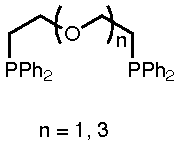
\includegraphics[]{../Figures/Alcock.pdf}
\caption[First reported POP pincer ligand]{First reported POP pincer ligand}
\label{Alcock}
\end{figure}

%Typically the central donor atom E is a carbon from an aromatic ring that binds through C-H activation to form a metallacycle.\cite{Choi2011}  

The different components of pincer ligands have significant influence on the steric and electronic properties and hence their reactivity.\cite{Singleton2003}  Altering the group X (Figure \ref{Pincerligands}) can lead to significant electronic effects mostly through the \emph{trans} influence.\cite{Choi2011}  For example, a carbon donor ligand has a greater \emph{trans} influence than an oxygen donor, so ligands \emph{trans} to X in PXP complexes will be bound more strongly when X~=~O than X~=~C.\cite{Zhu2008} The donor group Y controls the steric environment around the metal centre and the electron density.\cite{Choi2011}  Changing the backbone and other remote groups gives control over the electron density on the metal and can be used to improve solubility properties.\cite{Choi2011}

\begin{figure}[h]
\centering
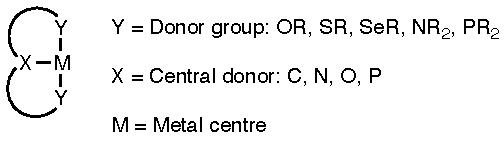
\includegraphics[]{../Figures/Pincerligands.pdf}
\caption[General representation of pincer ligands]{General representation of pincer ligands}
\label{Pincerligands}
\end{figure}

The tridentate coordination of pincer ligands, typically forming two five-membered metallacycles, imparts significant stability to metal complexes with pincer ligands.\cite{Choi2011}  The stability of the complexes is such that the backbone can undergo functionalisation at the 4-position to trimethylsilane \emph{via} lithiation with \emph{tert}-butyllithium and treatment with trimethylchlorosilane without inducing any decomposition of the platinum complex (Scheme \ref{Stability}).\cite{Albrecht2001}  This inherent stability allows the complexes to act as catalysts for highly endothermic reactions that require high temperatures, such as alkane dehydrogenation.\cite{Choi2011}

\begin{scheme}[h]
\centering
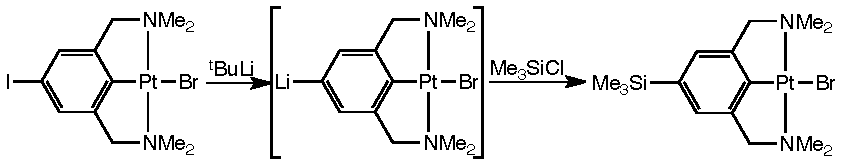
\includegraphics[]{../Schemes/Stability.pdf}
\caption[Functionalisation of an NCN pincer ligand]{Functionalisation of an NCN pincer ligand}
\label{Stability}
\end{scheme}

Coordination complexes of pincer ligands have a large number of applications.  Platinum complexes of an NCN pincer ligand have been utilised as sensors for the detection of sulfur dioxide.\cite{Albrecht2000, Albrecht2000c, Albrecht2001}  Palladium and nickel complexes of a number of pincer ligands have shown activity in cross-coupling reactions.\cite{Hahn2007, Bedford2000, Kimura2006, Zim2000, Obora2006} Theoretical studies have shown potential uses for pincer ligands in water-splitting\cite{Sandhya2011} and nitrogen fixation.\cite{Holscher2007}  However, one of the most prominent uses of pincer ligands is the activation of C-H bonds, typically as dehydrogenation catalysts.\cite{Choi2011, Albrecht2001, Crabtree2001}

%\subsection{Gas sensors}

%Platinum complexes of an NCN pincer (Figure \ref{Gassensors} \fixme{reference the structure correctly}) have been studied in solution or the crystalline state for use in the detection of sulfur dioxide.\cite{Albrecht2000, Albrecht2000c, Albrecht2001b}  In the presence of sulfur dioxide the square planar complex rapidly (less than 50 \si{\micro\second} adsorb the gas to form square pyramidal structures.\cite{Albrecht2000}  The adsorption is accompanied by a dramatic colour change from colourless to bright orange and is reversible upon exposure to a sulfur dioxide free atmosphere.\cite{Albrecht2000}  Dendrimer derivatives (2 and 3, Figure \ref{Gassensors}) can be used to detect sulfur dioxide at concentrations as low as 5 ppm (in a nitrogen atmosphere) \cite{Albrecht2001b}  

%\begin{figure}[h]
%\centering
%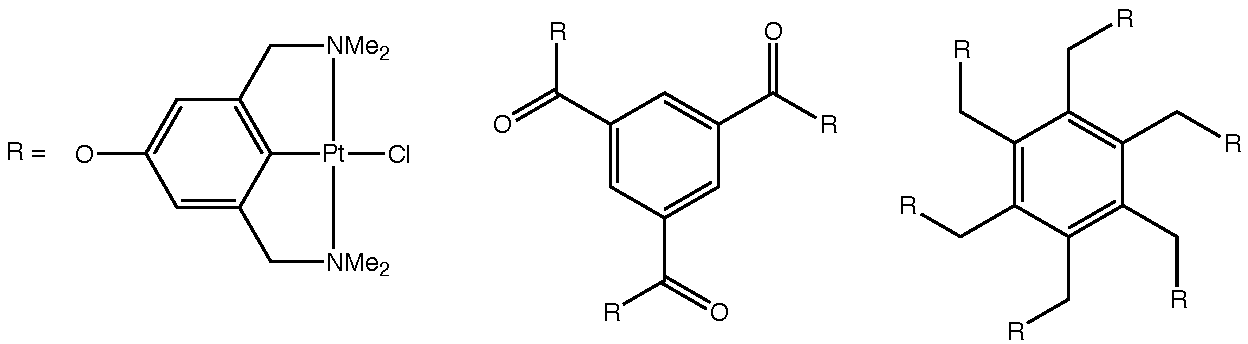
\includegraphics[width = \textwidth]{../Figures/Gassensors.pdf}
%\caption[NCN platinum complexes used for sensing \ce{SO2}]{NCN platinum complexes used for sensing \ce{SO2}}
%\label{Gassensors}
%\end{figure}

%These sensors have been studied further for physiological applications.  The complex (Figure \ref{Physiologicalgassensors}) is stable in both acidic and basic aqueous solutions for prolonged periods.\cite{Albrecht2000b}  Testing in conditions known to lead to rapid protein degradation (pH < 1, 50 \degrees C, 5 hours) results in no detectable decomposition.\cite{Albrecht2000b}  The coordination of sulfur dioxide to the complex results in a large shift in the $^{195}$Pt NMR of 1150 ppm (from -3150 to -2000 ppm).\cite{Albrecht2000b}  This could be detected by MRI for medical applications.  These complexes are also being developed for use as molecular switches for opto-electronics.\cite{Albrecht2000c}

%\begin{figure}[h]
%\centering
%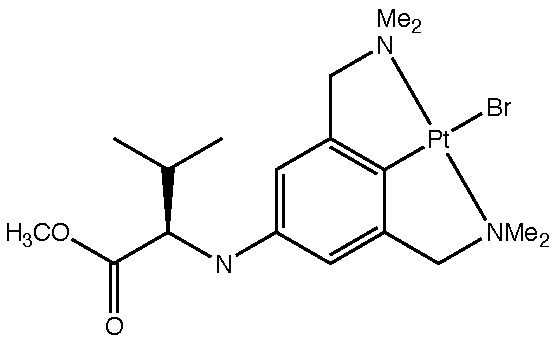
\includegraphics[height = 4.5cm]{../Figures/Physiologicalgassensors.pdf}
%\caption[NCN platinum complexes developed for \ce{SO2} sensing in physiological settings]{NCN platinum complexes developed for \ce{SO2} sensing in physiological settings}
%\label{Physiologicalgassensors}
%\end{figure}

%\subsection{Cross-coupling reactions}

%Coordination complexes of pincer ligands also find use as catalysts in carbon-carbon cross-coupling reactions such as the Suzuki, Heck \fixme{etc}.

%Pincer ligands with N-heterocyclic carbene (NHC) donors are becoming more common.\fixme{reference}  The palladium complexes found in figure \ref{CCCPincers} are active for the heck cross-coupling reaction of aryl bromides with styrene and the suzuki cross-coupling of aryl bromides with phenylboronic acid.\cite{Hahn2007}  Using a 1 mol \% catalyst loading the reaction of 4-bromobenzaldehyde and 4-bromoacetophenone with styrene quantitative yields were obtained after 24 hours regardless of the substituent on the ligand.  Using the \emph{n}-butyl derivatised ligand after two hours yields of 84.1, and 60.0 \% were obtained for reaction of styrene with 4-bromobenzaldehyde and 4-bromoacetophenone respectively.   The \emph{n}-butyl derived ligand formed an active palladium catalyst for the Suzuki cross-coupling of phenylboronic acid with 4-bromobenzaldehyde and 4-bromoacetophenone.  Using a 0.1 \% catalyst loading  yields of 50.7 and 48.7 \% respectively were obtained after two hours and quantitative conversion obtained in 24 hours.

%\begin{figure}[h]
%\centering
%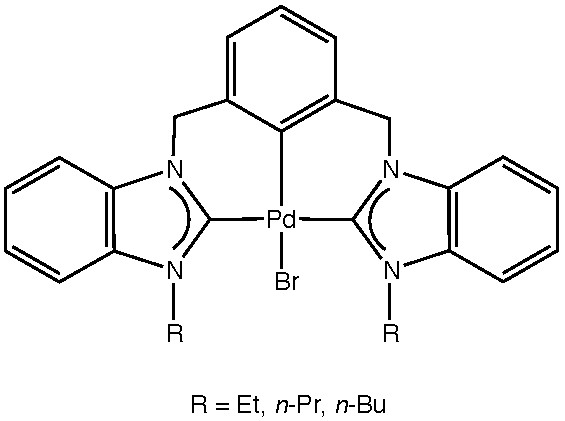
\includegraphics[height = 6 cm]{../Figures/CCCPincers.pdf}
%\caption[Palladium complexes with NHC donor pincer ligands]{Palladium complexes with NHC donor pincer ligands}
%\label{CCCPincers}
%\end{figure}

%The palladium complexes with ferrocene based PCP ligands (figure \ref{Ferrocenepalladium}) have been tested for activity in the Suzuki cross-coupling reaction.\cite{Sheloumov2008}  After 4.5 hours the reaction of 4-bromoacetophenone with phenylboronic acid in the presence of 1 and 3 was almost complete with 84 and 84.5 \% yields respectively under homogeneous conditions and quantitative yields under biphasic conditions (decane/\ce{H2O}).  The reaction was much slower with complex 2 with only 66 \% obtained after 15 hours.  Similar activities for all complexes were obtained for the homogeneous reaction of phenylboronic acid with 4-bromoanisole with yields of 77, 79 and 98 \% after 12, 15 and 15.5 hours for 1, 2 and 3 respectively.  However under biphasic conditions complex 2 was much less reactive obtaining a yield of 9 \% after 15 hours compared to 62 and 63.5 \% for 1 and 3 respectively.  The lower activity for complex 2 is thought to be due to the steric bulk of the \emph{tert}-butyl groups though in complex 3 the steric effect is overcome by the electronic influence of the Fe(III) rather than Fe(II).\cite{Sheloumov2008}

%See 

%\begin{figure}[h]
%\centering
%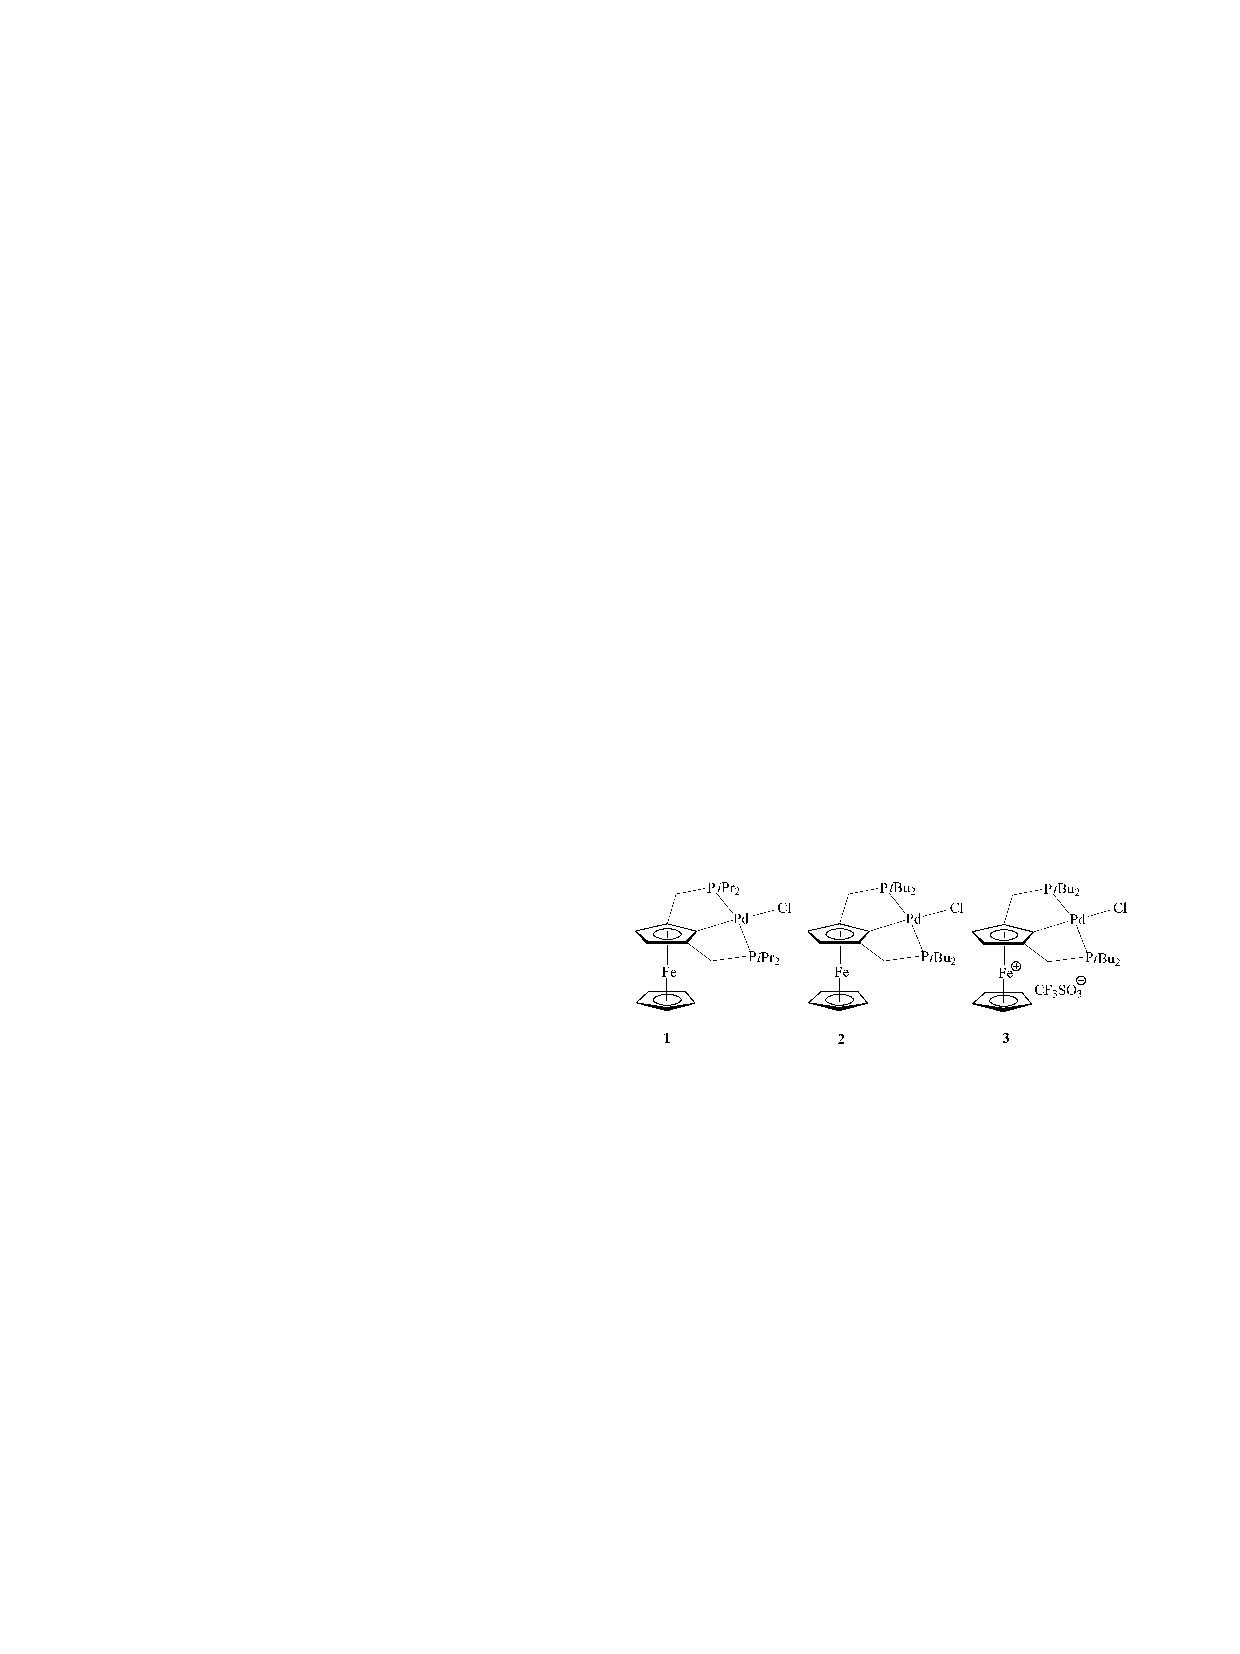
\includegraphics[height = 4.5cm]{../Figures/Ferrocenepalladium.pdf}
% \caption[Palladium complexes of ferrocene pincer ligands]{Palladium complexes of ferrocene pincer ligands}
%\label{Ferrocenepalladium}
%\end{figure}

%Definition\\	
%Naming\\
%Uses of the ligands\\
%Gas sensors\\
%SO2\\
%PCP\\
%POCOP\\
%PNP\\
%POP\\
%Nitrogen activation and fixation\\

\subsection{C-H activation}
%\subsection{Alkane dehydrogenation}

The catalytic dehydrogenation of alkanes has the potential to develop into an important industrial process allowing alkanes to be used as a chemical feedstock, without requiring high temperature cracking or other inefficient processes.\cite{Choi2011}  The first use of pincer complexes for alkane dehydrogenation was reported by Gupta in 1996.\cite{Gupta1996}  The rhodium and iridium dihydride complexes in figure \ref{Dehydrogenationligands} were tested for the dehydrogenation of cyclooctane in the presence of 3,3-dimethylbut-1-ene as hydrogen acceptor.  Rates of 0.8 turnovers h$^{-1}$ at 150~\degrees C were obtained for the rhodium complex, whilst the iridium complex was more active with rates of 82 turnovers h$^{-1}$.\cite{Gupta1996}  The catalysts used were highly stable at this temperature for extended periods and the addition of mercury did not inhibit the reaction indicating a homogeneous system.\cite{Gupta1996}  The higher activity of the iridium complex combined with the high thermal stability has led to a focus on iridium complexes for alkane dehydrogenation.\cite{Choi2011}

\begin{figure}[h]
\centering
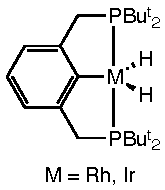
\includegraphics[]{../Figures/Dehydrogenationligands.pdf}
\caption[Rhodium and iridium pincer complexes used for alkane dehydrogenation]{Rhodium and iridium pincer complexes used for alkane dehydrogenation}
\label{Dehydrogenationligands}
\end{figure}

The iridium complex (Figure \ref{Dehydrogenationligands}) was also active for the dehydrogenation of cyclic alkanes, tetrahydrofuran and ethylbenzene to give arenes, furan and styrene respectively.\cite{Gupta1997, Gupta1997b}  In all cases the presence of excess 3,3-dimethylbut-1-ene as hydrogen acceptor inhibited the reaction so it was necessary to add this periodically.  A nitrogen atmosphere also inhibited reaction indicating competitive binding of nitrogen and alkane to the active site.\cite{Gupta1996, Gupta1997, Gupta1997b}  The iridium complex is also active for the dehydrogenation of cyclooctane and cyclodecane under acceptorless conditions.\cite{Xu1997}  A solution of fresh catalyst could be poisoned by addition of 10\% alkene rendering the catalyst inactive and indicating that the reduction of activity over time is not due to catalyst decomposition.\cite{Xu1997}

A mechanism for the alkane transfer dehydrogenation (Scheme \ref{Dehydrogenationcatalyticcycle}) has been elucidated \emph{via} a kinetics study by Goldman.\cite{Renkema2003}  The 3,3-dimethylbut-1-ene inserts into an iridium hydride bond, which is followed by reductive elimination to give the alkane.  The substrate undergoes oxidative addition to the iridium centre, which is followed by $\beta$-hydride elimination to give the alkene product and regenerate the iridium-dihydride.  With a limited concentration of 3,3-dimethylbut-1-ene (as is typical for these reactions) the rate determining step is the hydrogenation of the acceptor rather than C-H activation of the alkane, however with an excess of acceptor the rate determing step is the reaction with the cyclooctane.\cite{Renkema2003}  

\begin{scheme}[h]
\centering
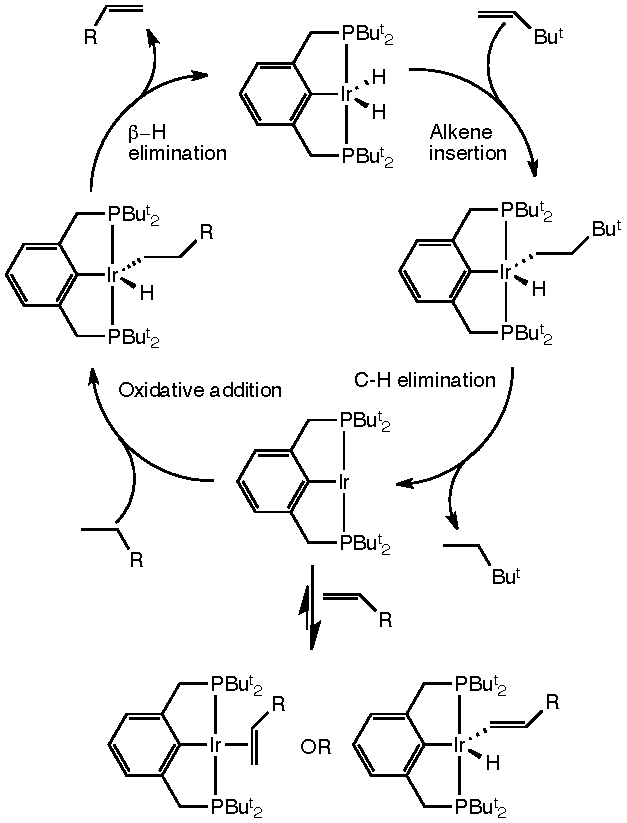
\includegraphics[]{../Schemes/Dehydrogenationcatalyticcycle.pdf}
\caption[Proposed mechanism for transfer dehydrogenation]{Proposed mechanism for transfer dehydrogenation}
\label{Dehydrogenationcatalyticcycle}
\end{scheme}

The three-coordinate [Ir(PCP)] intermediate formed following C-H elimination (Figure \ref{Dehydrogenationcatalyticcycle}) was proposed on the basis of an NMR study showing that the dihydride complex will react with 3,3-dimethylbut-1-ene to give the \emph{trans}-2-(\emph{tert}-butyl)vinyl complex that is in equilibrium with [Ir(PCP)] on an NMR timescale.\cite{Kanzelberger2000}  A more recent study has reported this resting state of the complex as the $\pi$-alkene complex and it is likely that both occur depending on the concentration of the hydrogen acceptor.\cite{Choi2011}  Studies into the acceptorless reaction have shown a similar mechanism.\cite{Krogh2002, Krogh2002b}  In this case the rate determining step is the thermolytic loss of \ce{H2} to give the active dehydrogenation complex [Ir(PCP)].  The inhibition of activity resulting from a build-up of alkene is likely due to the formation of the $\pi$-alkene complex and increased rate of the reverse reaction.\cite{Krogh2002, Krogh2002b}

Introduction of electron-donating groups such as \ce{OCH3} in the \emph{para}-position (Figure \ref{DFTpincers}) was shown to favour oxidative addition of an alkane to the 14-electron [Ir(PCP)] complex whilst disfavouring further addition of alkane to the \ce{[(PCP)Ir(R)(H)]} complex.\cite{Krogh2002c}  In the acceptorless dehydrogenation of cyclodecane at reflux (201 \degrees C) the electron-donating \ce{OCH3} pincer complex achieved 820 turnovers in 48 hours compared to 360 with a hydrogen in the \emph{para}-position.\cite{Zhu2004}   However, in dehydrogenation of \emph{n}-undecane at 196 \degrees C little difference was seen between the H and \ce{OCH3} substituted ligands with turnovers of 76 and 91 respectively after 4 hours.  The less sterically bulky isopropyl derivative (with \ce{OCH3} in the \emph{para}-position) was also tested and achieved 2970 turnovers over 48 hours for the dehydrogenation of cyclodecane, indicating that the steric bulk of the ligand has a significant influence of the rate of reaction.\cite{Zhu2004}   In the dehydrogenation of \emph{n}-undecane at 196~\degrees C the isopropyl catalyst was much less active than the \emph{tert}-butyl with only 30 turnovers achieved after 4 hours.  	

\begin{figure}[h]
\centering
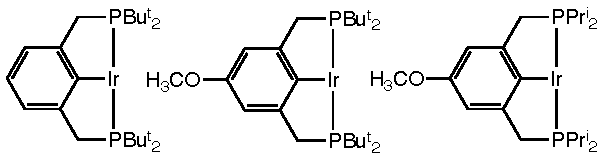
\includegraphics[]{../Figures/DFTpincers.pdf}
\caption[Electron-donating pincer ligands]{Electron-donating pincer ligands}
\label{DFTpincers}
\end{figure}

The steric environment imposed by the pincer ligand has a significant impact on the activity towards alkane dehydrogenation.\cite{Choi2011}  A computational and experimental study into this effect was reported by Brookhart in 2009.\cite{Kundu2009}  By exchanging the \emph{tert}-butyl groups on the xylene based PCP complex for methyl groups the impact of the sterically bulky \emph{tert}-butyl groups on alkane dehydrogenation could be studied.  Exchanging a single \emph{tert}-butyl results in a decrease in the transition state for the rate determining step ($\beta$-H elimination) of 42 kJmol$^{-1}$.  This was offset slightly by an increase of 17 kJmol$^{-1}$ in the bond strength of but-1-ene to the iridium centre.  Exchanging a second \emph{tert}-butyl for a methyl was calculated to have a much smaller overall impact as the but-1-ene bonds much more strongly to the metal centre.\cite{Kundu2009}  These results were supported experimentally in the transfer dehydrogenation of \emph{n}-octane using 3,3-dimethylbut-1-ene as the acceptor.  With one and two methyls replacing \emph{tert}-butyl groups, 195 and 140 turnovers were obtained respectively, compared to only 53 for the unmodified ligand.\cite{Kundu2009}

Although the PCP iridium complexes are stable at 150 \degrees C for extended periods, significant decomposition becomes apparent after 24 hours at 200 \degrees C.\cite{Gupta1996}  Ligands based on an anthracene backbone (Figure \ref{Anthraphos}) were developed to achieve a higher level of thermal stability.\cite{Haenel2001}  The ``anthraphos'' ligand forms thermally stable complexes with decomposition occurring at 308 \degrees C for the iridium dihydride complex.  However, in the catalytic dehydrogenation of cyclodecane at 150 \degrees C the complex was less active than the xylene-based systems.  It was proposed that the lack of flexibility in the backbone of anthraphos was responsible for the decreased activity.\cite{Haenel2001}

\begin{figure}[h]
\centering
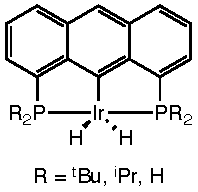
\includegraphics[]{../Figures/Anthraphos.pdf}
\caption[Iridium anthraphos complexes tested for catalytic dehydrogenation]{Iridium anthraphos complexes tested for catalytic dehydrogenation}
\label{Anthraphos}
\end{figure}

The bis-phosphinite (POCOP) pincer ligands in Figure \ref{Phosphinite} were reported independently by Brookhart (R = \ce{^{t}Bu}, X = \ce{OCH3}, \ce{CH3}, H, F, \ce{C6F5}, ArF)\cite{Gottker2004, Gottker2004b} and Jensen (R~=~\ce{^{i}Pr}, X = H) in 2004.\cite{Morales2004}  Brookhart's complexes were tested for activity in the transfer dehydrogenation of cyclooctane at 200 \degrees C using 3,3-dimethylbut-1-ene as hydrogen acceptor.  These complexes displayed high turnover numbers of up to 2041 after 40 hours forming both cyclooctene and 1,3-cyclooctadiene.\cite{Gottker2004}  The cyclooctadiene product spontaneously converts (most likely \emph{via} a disrotatory ring closure of cyclooctatriene) into \emph{o}-xylene and ethylbenzene (Scheme \ref{Benzeneformation}).\cite{Gottker2004}

\begin{figure}[h]
\centering
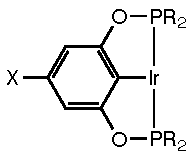
\includegraphics[]{../Figures/Phosphinite.pdf}
\caption[Iridium POCOP complex]{Iridium POCOP complex}
\label{Phosphinite}
\end{figure}

\begin{scheme}[h]
\centering
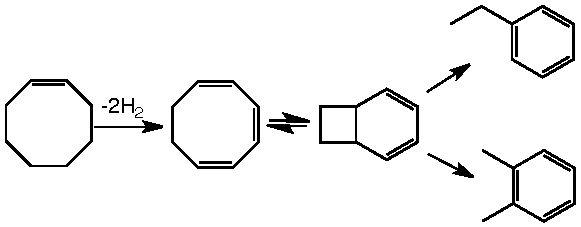
\includegraphics[]{../Schemes/Benzeneformation.pdf}
\caption[Reaction of cyclooctene to form alkylbenzenes]{Reaction of cyclooctene to form alkylbenzenes}
\label{Benzeneformation}
\end{scheme}

The electronic influence of the pincer ligand can also have a dramatic impact on the catalytic activity.  A ruthenium PCP complex with electron-withdrawing \ce{CF3} substituents on the phosphorus atoms (Figure \ref{ElectronwithdrawingPCP}) was tested for transfer and acceptorless dehydrogenation of cyclooctane.\cite{Gruver2011}  The catalyst achieved 186 turnovers at 200 \degrees C after only 30 minutes of transfer dehydrogenation and 10 turnovers in 60 minutes under acceptorless conditions.  This complex was prone to decomposition due to the high temperatures used.  However, the presence of oxygen, nitrogen and water resulted in no significant change to the catalysis which is a significant advantage over other systems.  

\begin{figure}[h]
\centering
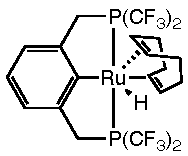
\includegraphics[]{../Figures/ElectronwithdrawingPCP.pdf}
\caption[Ruthenium complex of an electron-withdrawing PCP ligand]{Ruthenium complex of an electron-withdrawing PCP ligand}
\label{ElectronwithdrawingPCP}
\end{figure}

Pincer complexes based on metallocenes have also been synthesised and tested for use in alkane dehydrogenation (Figure \ref{Metallocenepincers}).\cite{Kuklin2006}  These complexes have much higher activity than those previously reported.  Turnover numbers of 3300 and 2571 were obtained after eight hours for the iron and ruthenium metallocenes, respectively in the transfer dehydrogenation of cyclooctane with 3,3-dimethylbut-1-ene as hydrogen acceptor at 180 \degrees C.  This compares with 1843 for the iridium POCOP pincer complex (Figure \ref{Phosphinite}) when tested in the same conditions.  The increased activity was proposed as being due to less steric hindrance of the metal centre compared to the POCOP complex.\cite{Kuklin2006}

\begin{figure}[h]
\centering
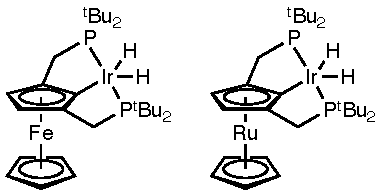
\includegraphics[]{../Figures/Metallocenepincers.pdf}
\caption[Metallocene based pincer ligands]{Metallocene based pincer ligands}
\label{Metallocenepincers}
\end{figure}

\subsection{Alkane metathesis}

Alkene metathesis is a well-known chemical transformation where the groups of two alkenes are exchanged in the presence of an appropriate catalyst.\cite{Astruc2005}  Alkane metathesis follows the same general principle; the exchange of alkane fragments to produce an array of longer and shorter alkanes.\cite{Choi2011}  Although this was first studied from a heterogeneous perspective,\cite{Burnett1973, Vidal1997, Basset2005} more recently homogeneous pincer complexes have been utilised.\cite{Goldman2006}

%Shell higher olefins process

The first alkane metathesis catalysts were heterogeneous mixtures of dehydrogenation/ hydrogenation and metathesis catalysts.\cite{Burnett1973, Vidal1997}   A mixture of tungsten oxide on silica and platinum metal on alumina formed an active alkane metathesis catalyst.\cite{Burnett1973}  The platinum metal dehydrogenates the alkane, which then reacts in an alkene metathesis reaction, followed by hydrogenation by the platinum to form shorter and longer alkanes.  When exposed to \emph{n}-butane a mixture of 24.7, 37.6, 15.9 and 8.6\% of \ce{C3}, \ce{C4}, \ce{C5} and \ce{C6} linear alkanes was obtained with small amounts of branched and higher alkanes.  However, this system required high temperature (400 \degrees C) and was very sensitive to poisoning by water, ammonia, oxygen and hydrogen sulfide.\cite{Burnett1973}

A tantalum hydride catalyst on silica was more successful with catalysis occuring at room temperature.\cite{Vidal1997}  This system followed a slightly different mechanism, shown in Scheme \ref{Tantalumcatalyticcycle}.  The first step involves coordination to the tantalum \emph{via} loss of hydrogen gas.  This is followed by addition of further alkane to form a metallacycle intermediate that rearranges to give the longer chain product and a tantalum methyl species.  This can react with further alkane to form methane and regenerate the catalytic tantalum alkyl species.  This system is active towards a number of alkanes giving a statistical distribution of longer and shorter alkanes, however the turnover numbers obtained were low; 46, 47, 66, 17 and 12 for ethane, propane, butane, isobutane and pentane respectively.\cite{Vidal1997}

\begin{scheme}[h]
\centering
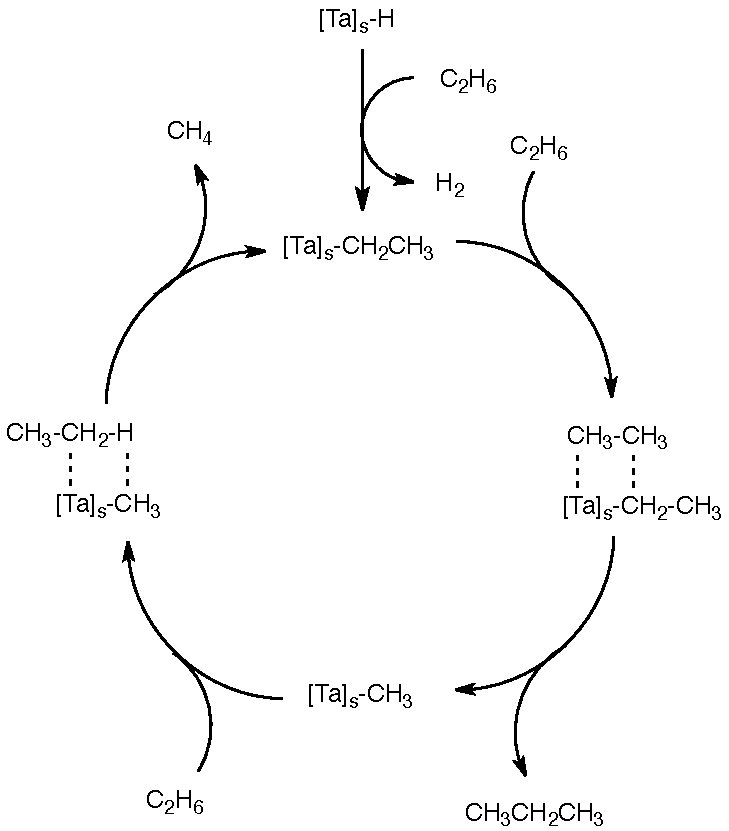
\includegraphics[width = 0.7\textwidth]{../Schemes/Tantalumcatalyticcycle.pdf}
\caption[Catalytic cycle for alkane metathesis by a heterogeneous tantalum catalyst]{Catalytic cycle for alkane metathesis by a heterogeneous tantalum catalyst}
\label{Tantalumcatalyticcycle}
\end{scheme}

The use of pincer complexes for alkane metathesis has typically followed the tandem alkane dehydrogenation and alkene metathesis protocol (Scheme \ref{Tandemmetathesis}).\cite{Choi2011} Combining an iridium pincer dehydrogenation catalyst with the Schrock alkene metathesis catalyst (Figure \ref{PCPSchrock}) gave active catalysts with turnover numbers of 135, 205 and 125 after 24 hours for the conversion of \emph{n}-hexane using pincer complexes (a) (with L = \ce{C2H4}, \ce{H2}) and (b) respectively.\cite{Goldman2006}  The activity was limited by degradation of the alkene metathesis catalyst as reaction resumed upon further addition of Schrock's catalyst.  A major advantage of this catalytic system is the selective formation of linear alkanes as no branched or cyclic alkanes were detected.\cite{Goldman2006}

\begin{scheme}[h]
\centering
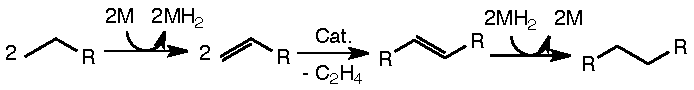
\includegraphics[]{../Schemes/Tandemmetathesis.pdf}
\caption[Alkane metathesis \emph{via} transfer hydrogenation and alkene metathesis]{Alkane metathesis \emph{via} transfer hydrogenation and alkene metathesis}
\label{Tandemmetathesis}
\end{scheme}

\begin{figure}[h]
\centering
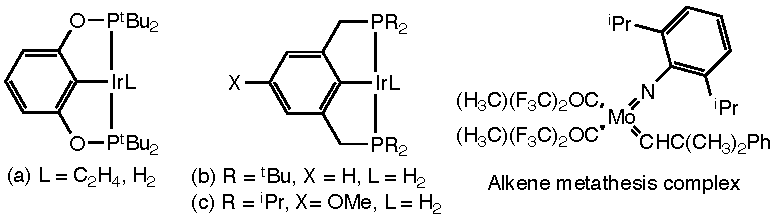
\includegraphics[]{../Figures/PCPSchrock.pdf}
\caption[Transfer hydrogenation and alkene metathesis catalysts]{Transfer hydrogenation and alkene metathesis catalysts}
\label{PCPSchrock}
\end{figure}

Replacement of Schrock's catalyst with a heterogeneous alkene metathesis catalyst was tested to increase the stability.  This \ce{Re2O7}/\ce{Al2O3} catalyst was more stable than Schrock's catalyst and showed a higher level of activity with 125 turnovers achieved with complex (b) (Figure \ref{PCPSchrock}) and 180 for complex (c) in 3 hours for the conversion of \emph{n}-decane.\cite{Goldman2006}  However, the activity of the phosphinite complexes was reduced with (a) achieving only 15 turnovers in 3 hours.  Although a high level of selectivity with complexes (b) and (c) for terminal alkenes has been reported for the dehydrogenation,\cite{Liu1999} the product distribution (Figure \ref{GCdistribution})  shows no preference for ethane, which would occur if this was the case.  Either isomerisation of the terminal alkene to form internal alkenes prior to metathesis, or further reaction of the alkane products must occur to account for the observed product distribution.\cite{Goldman2006, Choi2011}

\begin{figure}[h]
\centering
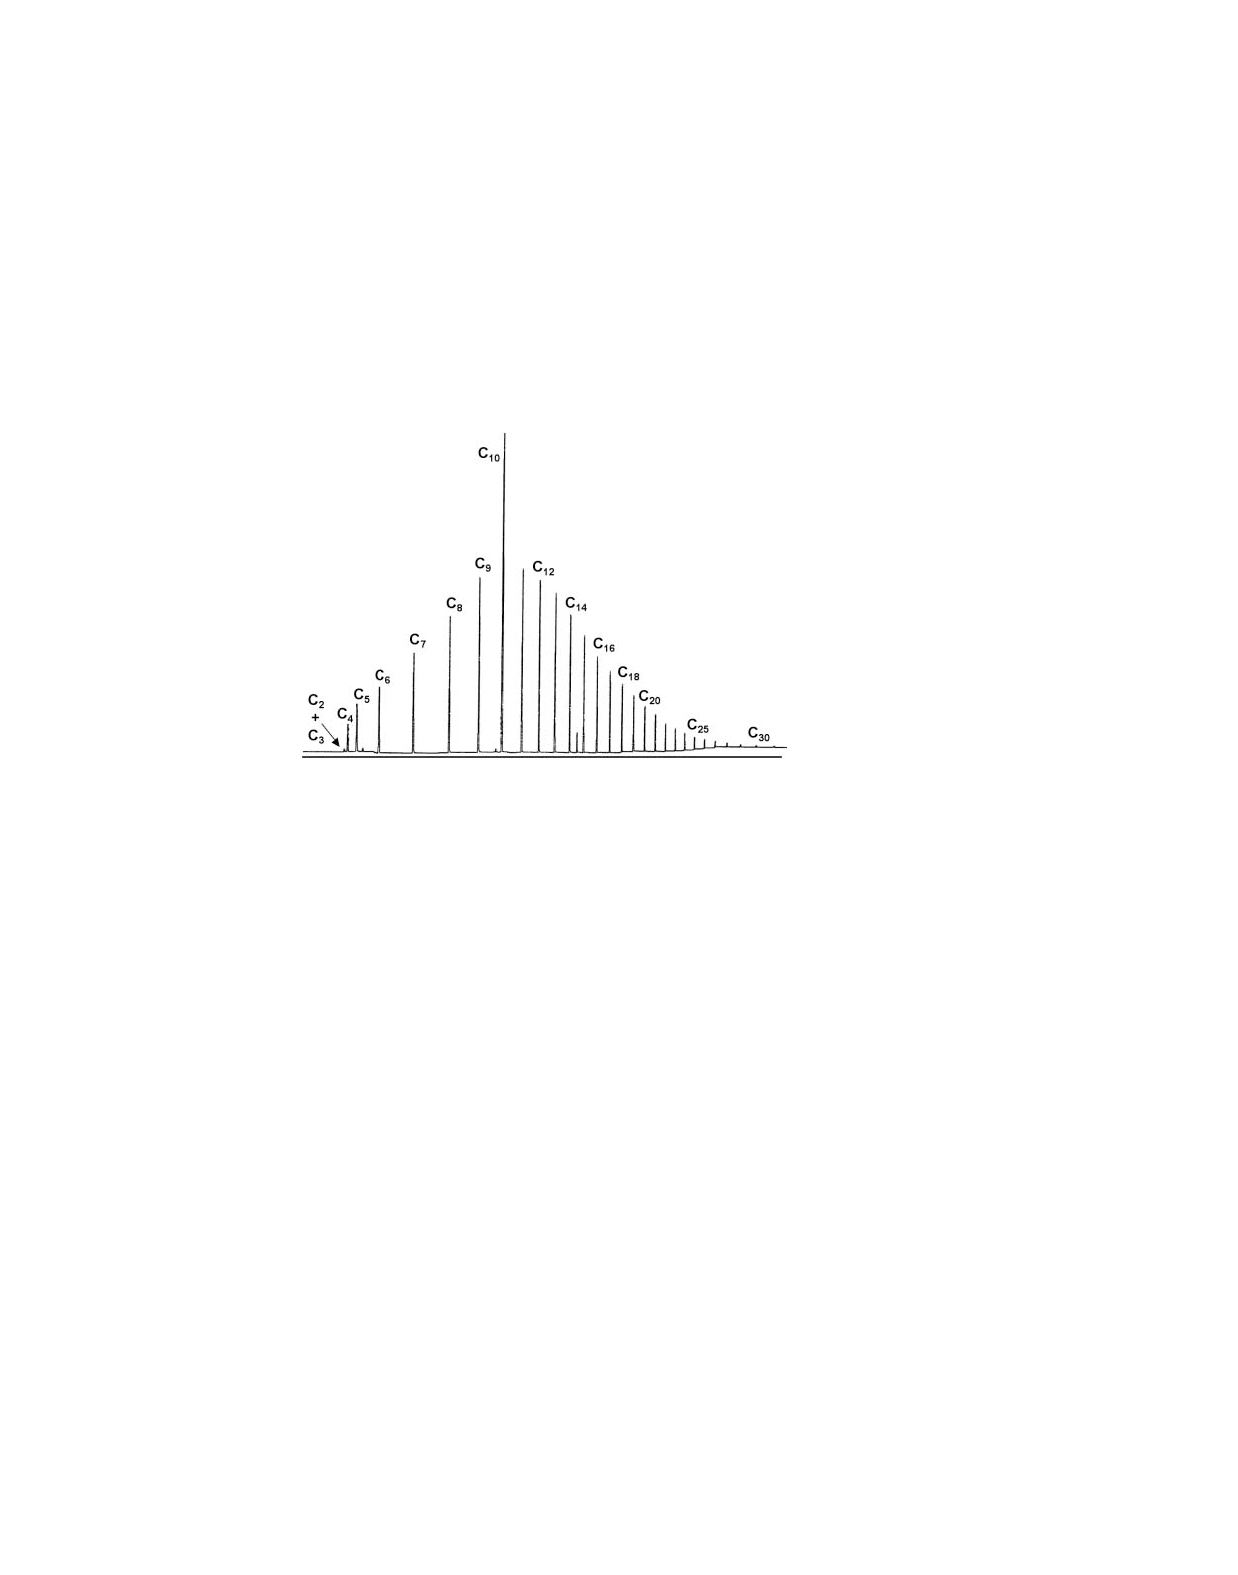
\includegraphics[width = 0.65\textwidth]{../Figures/GCdistribution.pdf}
\caption[GC trace of products obtained from alkane metathesis of \emph{n}-decane]{GC trace of products obtained from alkane metathesis of \emph{n}-decane reproduced from Goldman et al.\cite{Goldman2006}}
\label{GCdistribution}
\end{figure}

\subsection{POP pincer ligands}

Although one of the first pincer ligands reported was a POP pincer,\cite{Alcock1976} this type of ligand has not been studied as extensively as the PCP and PNP analogues.  The osmium trichloride complex of \gls{dbf}(P$^i$\ce{Pr2)2} (Figure \ref{Osmiumdbf}) formed in 98\% yield when the ligand was reacted with the commercially available \ce{OsCl3}$\cdot{}$3\ce{H2O} under reflux.\cite{Asensio2010}  When the ligand is reacted with \ce{OsCl2(DMSO)4} (DMSO = dimethylsulfoxide) the \emph{trans}-dichloro \gls{DMSO} complex (Scheme \ref{Osmiumdbfscheme}) is formed.\cite{Esteruelas2011} This complex can be converted to trihydridechloride and tetrahydride osmium complexes upon reaction with hydrogen gas in the presence of triethylamine or sodium hydrid,e respectively.  The tetrahydride complex is an active catalyst for the coupling of amines and alcohols to give imines achieving a 98\% yield after 3 hours for the coupling of benzyl alcohol and aniline.  Lower yields of 49 and 54\% were obtained when the \gls{DMSO} and trihydride complexes were used.\cite{Esteruelas2011}

\begin{figure}[h]
\centering
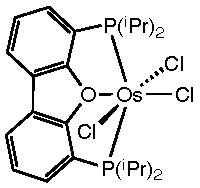
\includegraphics[]{../Figures/Osmiumdbf.pdf}
\caption[Osmium trichloride complex of \ce{dbf(P^{i}Pr2)2}]{Osmium trichloride complex of \ce{dbf(P^{i}Pr2)2}}
\label{Osmiumdbf}
\end{figure}

\begin{scheme}[h]
\centering
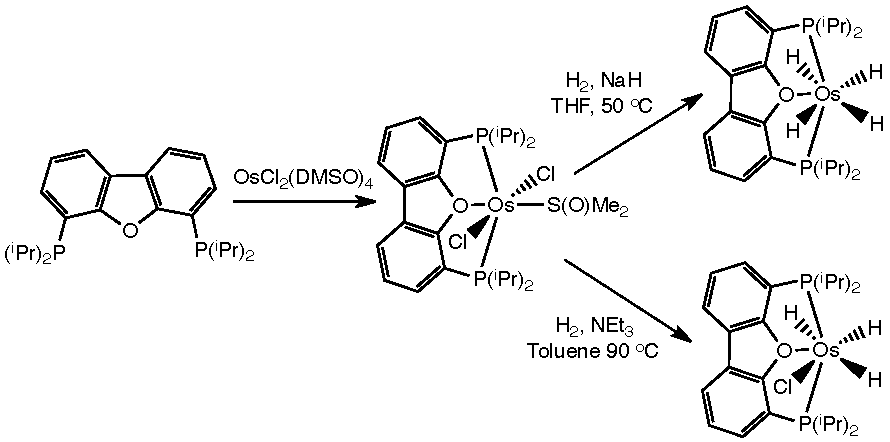
\includegraphics[]{../Schemes/Osmiumdbfscheme.pdf}
\caption[Reaction of osmium complexes of \ce{dbf(P^{i}Pr2)2}]{Reaction of osmium complexes of \ce{dbf(P^{i}Pr2)2}}
\label{Osmiumdbfscheme}
\end{scheme}

A theoretical study has suggested that POP pincers could be utilised as ligands for ruthenium catalysed synthesis of ammonia from nitrogen and hydrogen gases.\cite{Holscher2007}  The PNP and PSP ligands (Figure \ref{Theoreticalammonia}) have much higher activation barriers for the formation of the active catalytic species than the POP ligands.  Theoretical studies into Shilov chemistry have shown that the presence of an oxygen or nitrogen ligand \emph{trans} to the methane results in much lower activation barriers.\cite{Zhu2009}  The two-step process for C-H activation involves the loss of a ligand followed by coordination of the methane.  The C-H activation has no discernible energy barrier when an oxygen ligand is present in the \emph{trans}-position, however the intial loss of the ligand is much faster for ligands with a higher \emph{trans}-influence making the nitrogen donors much better overall.  Given a system where other factors promoted the loss of the ligand (such as steric bulk) it may be possible that the oxygen-donor ligands are better overall.  

\begin{figure}[h]
\centering
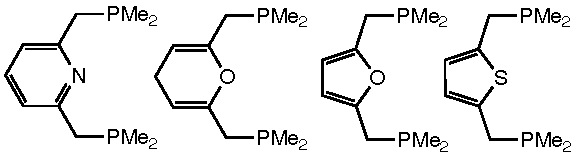
\includegraphics[]{../Figures/Theoreticalammonia.pdf}
\caption[Pincer ligands studied for catalytic ammonia synthesis]{Pincer ligands studied for catalytic ammonia synthesis}
\label{Theoreticalammonia}
\end{figure}

Research into the effect of different phosphorus substituents on the reactivity of ruthenium POP pincer complexes has been reported.\cite{Major2005}  Reaction of \ce{[RuCl2(}\emph{p}-\ce{cymene)]2} (\gls{cymene} = 1-methyl-4-(1-methylethyl)benzene) with the sterically bulky POP-\ce{^{t}}Bu yielded the five-coordinate complex, [Ru\ce{Cl2}(POP)] (Scheme \ref{RutheniumPOP}).  However, the less bulky POP-\ce{^{i}Pr} formed a dimeric species.  Both species were able to form molecular hydrogen complexes however, with the POP-\ce{^{i}}Pr, the \ce{H2} occupies the site \emph{trans} to the ether whilst it occupies the site \emph{trans} to chloride with the bulkier POP-\ce{^{t}}Bu.  The difference was ascribed to the \ce{H2} occupying the most sterically restrained site in the presence of the POP-\ce{^{t}}Bu as it is the smallest ligand (based on van der Waals radii).  

\begin{scheme}[h]
\centering
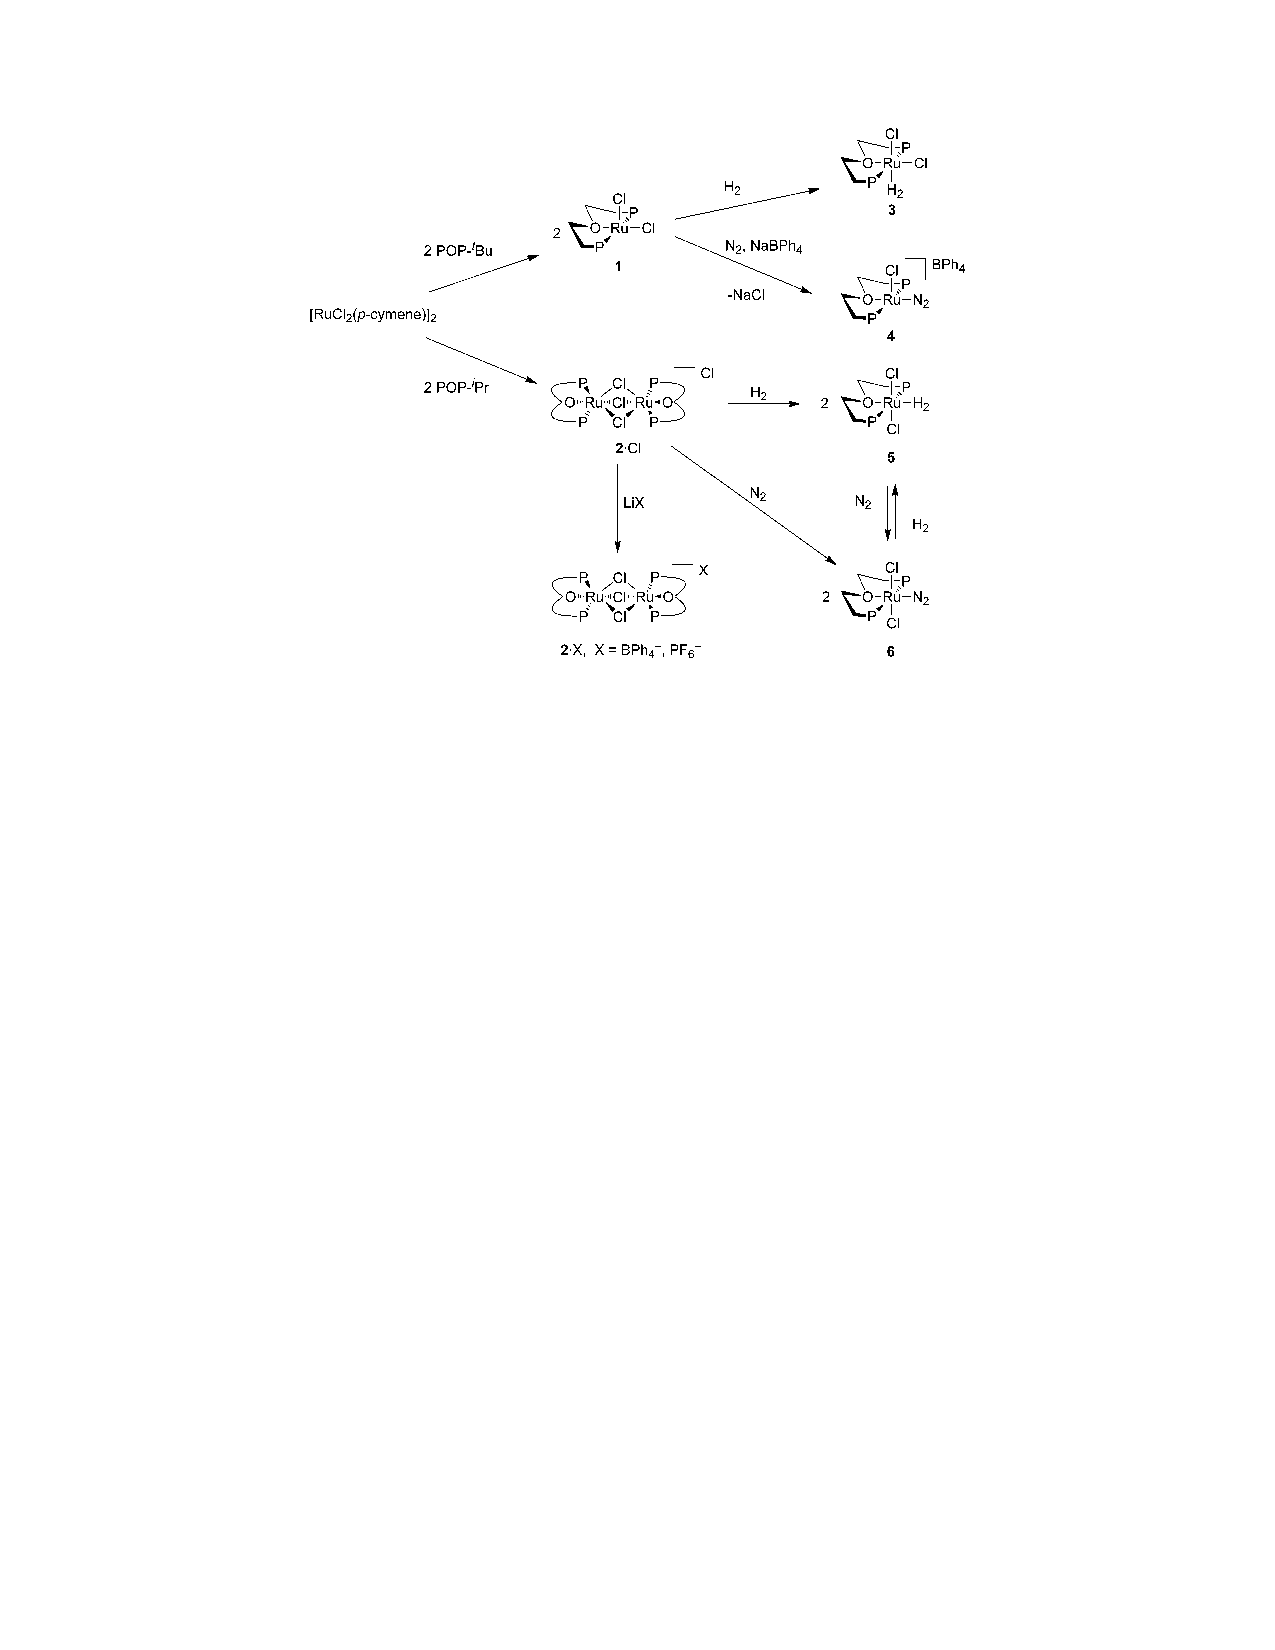
\includegraphics[width = \textwidth]{../Schemes/RutheniumPOP.pdf}
\caption[Reactivity of ruthenium POP complexes]{Reactivity of ruthenium POP complexes}
\label{RutheniumPOP}
\end{scheme}

The different reactivity was also observed in reaction of the complexes with nitrogen (Scheme \ref{RutheniumPOP}).\cite{Major2005}  The less bulky POP-\ce{^{i}}Pr formed a complex analogous to the molecular hydrogen complex and the two were readily interconverted.  However, the bulky POP-\ce{^{t}}Bu did not react spontaneously with nitrogen and required chloride abstraction using \ce{NaBPh4} in order to form the five-coordinate complex [RuCl\ce{N2}(POP)]\ce{BPh4}.

%See crabtree2001 for the use of pincers in alkane dehydrogenation
%Cundari papers for methane activation DFT studies
	%Methane activation to Ir(PH3)2Cl is 29 kcal mol-1 more exothermic than addition to the hydride complex
%Krogh2002 in the conclusion says that the influence of electron donating ancillary is very minor

POP ligands also have the potential for hemilability of the central donor group whereby the oxygen can bind reversibly to the metal centre in order to stabilise catalytic intermediates. This has been utilised in the hydroacylation of alkenes and alkynes using a rhodium pincer complex, where the oxygen can bind in order to stabilise important intermediates and prevent the competing decarbonylation reactions from occuring.\cite{Moxham2006, Moxham2008, Pawley2010}  A range of rhodium complexes with \gls{xantphos} or \gls{DPEphos} as ancillary diphosphine ligands were tested for the hydroacylation reaction.\cite{Moxham2006}  The \gls{DPEphos} complexes were more active than the \gls{dppe} complex used for comparison, achieving conversions of 100\% after 30 min and 90 min respectively.  However, the xantphos complex was completely inactive.  The different reactivity is thought to be a result of the flexibility of the backbone.\cite{Pawley2010}  The more flexible \gls{DPEphos} readily exhibits hemilability whilst the less flexible xantphos can form either tridentate or bidentate complexes but does not readily convert between the two.\cite{Moxham2006, Pawley2010}  Utilising a PCP pincer resulted in decomposition whilst a PSP pincer bound too strongly to the metal to allow catalysis to occur.\cite{Moxham2008}

\subsection{Xantphos}
	
First reported in 1995 by Kranenburg et al.,\cite{Kranenburg1995} the diphosphine ligand \gls{xantphos} and its derivatives (Figure \ref{Xantphosligands}) were designed to investigate the influence of the bite angle on catalytic reactions, in particular rhodium catalysed hydroformylation.  The bite angle is the angle between the two phosphorus atoms on the diphosphine and the metal centre as shown in Figure \ref{Biteangle}. Utilising different backbones such as diphenyl ether or dibenzofuran, or varying the group in the xantphos backbone to S, \ce{SiMe2} or \ce{CMe2} altered the sterics of the ligand resulting in a change in the bite angle (Table \ref{Biteangletable}).\cite{Kranenburg1995} 

\begin{figure}[h]
\centering
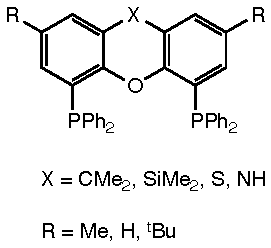
\includegraphics[]{../Figures/Xantphos.pdf}
\caption[The xantphos class of ligands]{The xantphos class of ligands}
\label{Xantphosligands}
\end{figure}

\begin{figure}[h]
\centering
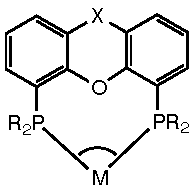
\includegraphics[]{../Figures/Biteangle.pdf}
\caption[The bite angle]{The bite angle}
\label{Biteangle}
\end{figure}

\begin{table}[h]
\caption[Calculated bite angles for xantphos-type ligands]{Calculated bite angle for xantphos-type ligands}
\label{Biteangletable}
\begin{center}
    \begin{tabular}{l l l}
    \hline
Backbone		& Bite angle (\degrees)	& Flexibility range	\\ \hline
\ce{CMe2}	& 111.7				& 97 - 135\\
S			& 109.4				& 94 - 130\\
\ce{SiMe2}	& 108.7				& 93 - 132\\
DPEphos		& 102.2				& 86 - 120\\
dbfphos		& 131.1				& 117 - 147\\
    \hline
    \end{tabular}
    \end{center} 
    \end{table}

In the hydrocyanation of styrene, ligands with bite angles close to 105\degrees~resulted in high yields and selectivities whilst decreasing the bite angle to 101\degrees or increasing to 110\degrees~led to a much lower activity.\cite{Kranenburg1995b}  The bite angle is thought to influence the reaction by stabilising preferred reaction intermediates and destabilising inactive species.   In the hydrocyanation reaction the bite angle close to 109\degrees~ destabilises square-planar Ni(II) species and stabilises the tetrahedral Ni(0) species, enhancing the reductive elimination step and resulting in a faster reaction.\cite{Kranenburg1995b}

Since the initial studies in hydroformylation and hydrocyanation, transition metal complexes of xantphos and its derivatives have been investigated for use in a range of catalytic systems including allylic alkylation,\cite{Kranenburg1998} CO/ethene copolymerisation,\cite{Freixa2003} and C-C and C-X cross-coupling reactions\cite{Birkholz2009} among others.  In addition, a range of further derivatives of xantphos have been synthesised.  Rhodium complexes of the water-soluble xantham\cite{Buhling1997} and sulfoxantphos (Figure \ref{Xantham}) have been used for biphasic hydroformylation.\cite{Goedheijt1998}

\begin{figure}[h]
\centering
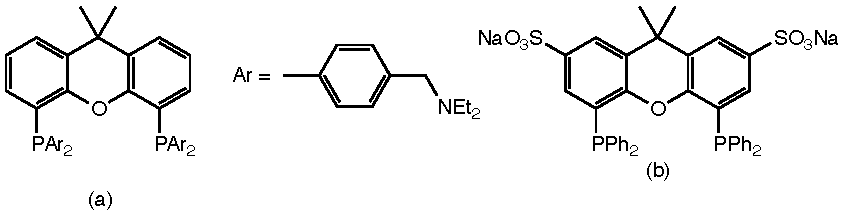
\includegraphics[]{../Figures/Xantham.pdf}
\caption[Water soluble xantphos ligands]{Water soluble xantphos ligands (a) Xantham, (b) Sulfoxantphos}
\label{Xantham}
\end{figure}

Xantphos has a range of potential binding modes (Figure \ref{Xantphosbinding}).  By far the most common is the \emph{cis}-bidentate chelating mode (a) with both phosphorus atoms bonding to the metal.  Less commonly the \emph{trans}-bidentate chelating diphosphine mode (b) is observed.  A third, tridentate binding mode (c) is also possible where the oxygen binds in addition to the two phosphorus atoms.  A recent search of the Cambridge Crystallographic Database revealed 107 X-ray crystal structures of coordination complexes with xantphos derived ligand of these only five exhibited the tridentate binding mode.  A monodentate binding mode is also possible, though it is very rare with only one crystal structure reported to date.\cite{Escalle2009}

\begin{figure}[h]
\centering
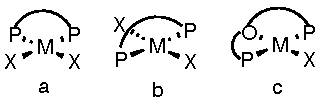
\includegraphics[height = 2.5cm]{../Figures/Xantphosbinding.pdf}
\caption[Possible bonding modes of xantphos ligands]{Possible bonding modes of xantphos ligands (a) \emph{cis}-bidentate chelate, (b) \emph{trans}-bidentate chelate, (c) tridentate chelate}
\label{Xantphosbinding}
\end{figure}

Ruthenium complexes of xantphos have been utilised for the activation of dihydrogen to form dihydride complexes (Scheme \ref{Xantphosdihydrogen}).\cite{Lenero2003}  Reaction of [Ru(cod)(cot)] (\gls{cot} = 1,3,5-cyclooctatriene) with the diphosphine in a hydrogen atmosphere led to the formation of the \emph{cis}-dihydride.  Protonation of this complex at low temperature (183 K) formed a molecular hydrogen complex that could eliminate hydrogen gas when allowed to warm to 233 K.  

\begin{scheme}[h]
\centering
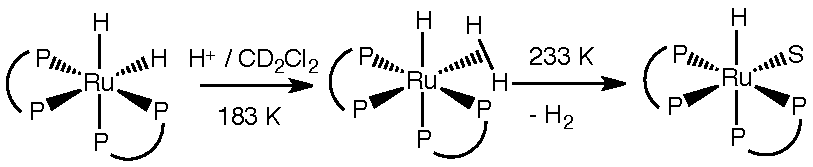
\includegraphics[width = 0.9\textwidth]{../Schemes/Xantphosdihydrogen.pdf}
\caption[Reactions of ruthenium hydride complexes]{Reactions of ruthenium hydride complexes}
\label{Xantphosdihydrogen}
\end{scheme}

Xantphos and DPEphos ruthenium complexes displaying the tridentate binding mode exhibit reversible bonding of dihydrogen and dinitrogen, together with irreversible binding of peroxide (Scheme \ref{Gascomplexes}).\cite{Ledger2010}  The molecular hydrogen and nitrogen complexes form upon exposure of a dichloromethane solution of the complex to 1 atm of the appropriate gas at low temperature (180 K).  These complexes were unstable and degraded when exposed to higher temperature.  The peroxide complexes form spontaneously on exposure of a dichloromethane solution to air and are stable under ambient conditions.

\begin{scheme}[h]
\centering
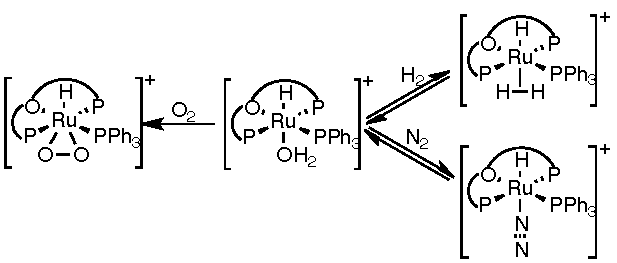
\includegraphics[]{../Schemes/Gascomplexes.pdf}
\caption[Ruthenium xantphos complexes of oxygen, hydrogen and nitrogen]{Ruthenium xantphos complexes of molecular oxygen, hydrogen and nitrogen}
\label{Gascomplexes}
\end{scheme}

%\fixme{xantphos use as a pincer ligand}\\
%Osmium, Asensio2010, Esteruelas2011\cite{Asensio2010, Esteruelas2011}\\
%Ruthenium, Ledger2010\cite{Ledger2010}

%%!TEX root = Thesis.tex

\chapter{Research Proposal}
\label{ch:proposal}

Pincer compounds have found significant use as ligands in a number of catalytic applications.  However, the main focus has been on PCP compounds.  Although the first POP and PCP ligands were reported in the same year,\cite{Moulton1976, Alcock1976} significantly more research has been carried out on PCP ligands.  However, POP ligands have a number of potential advantages over their PCP counterparts.  Late transition metals are very electron rich so will form a much weaker bond with an ether-based POP ligand than with a PCP donor.\cite{Zhu2008}  This weaker metal-oxygen bond will result in stronger bonds \emph{trans} to oxygen.  Given that methane is a very poor $\sigma$-donor and $\pi$-acceptor ligand, it forms very weak complexes with a metal centre.\cite{Crabtree2001}  Theoretical studies into the platinum catalysed Shilov hydroxylation of methane have shown that oxygen donor ligands \emph{trans} to the alkane significantly reduce the energy barrier associated with C-H activation.\cite{Zhu2009} 

%Hence the use of a POP ligand will allow for the formation of $\sigma$-methane complexes with a higher stability than that previously reported.  This will allow further study into the nature of the bonding and complexes that occur as in $\sigma$-methane complexes that are often proposed as intermediates in catalytic C-H activation.  In addition the weak metal-oxygen bond has the potential for hemilability which has been utilised in the hydroacylation of alkene and alkynes.\cite{Moxham2006}

The other donor groups in the pincer compound are particularly important in controlling the steric and electronic environment of the metal centre.\cite{Choi2011}  The use of electron donating groups will increase the electron density of the metal and enhance $\pi$-back bonding into the $\sigma$* orbital of methane, thus decreasing the bond order and promoting oxidative addition of methane to the metal.\cite{Crabtree2001}  However, electron-withdrawing diphosphinite pincer ligands have been the subject of much research recently, in particular in the formation of $\sigma$-methane complexes.\cite{Bernskoetter2009}

Late transition metals, in low oxidation states do not readily form bonds with oxygen donor ligands.\cite{Davies1981}  As such, POP ligands have the potential to act as hemilabile ligands forming tridentate pincer complexes with higher oxidation states and diphosphine complexes with metals in low oxidation states, thus stabilising a number of potential intermediates in catalytic systems.\cite{Moxham2006, Moxham2008}  In addition, this has the potential to overcome a major problem with pincer ligands in that they have a large energy barrier to undergo rearrangement as required by some catalytic systems such as alkane dehydrogenation.\cite{Wang1996}

\section{Proposal}

The POP ligands investigated will be based on the xantphos ligands reported by Kranenburg and coworkers.\cite{Kranenburg1995}  These ligands have been shown to bind in a tridentate pincer fashion, though the preferred mode is the bidentate P-P.\cite{Nieczypor2001, Turculet2007, Sandee1999, Zuideveld2002}  Specifically the ligands to be investigated (Figure \ref{Proposedligands}) will be based on the xantphos, thioxantphos and sixantphos backbones with pentafluorophenyl or \emph{tert}-butyl groups on the phosphines.  Previous work has suggested that electron-rich metals are more active for oxidative addition, however the electron-withdrawing diphosphinite PONOP pincers can form long-lived $\sigma$-methane complexes\cite{Bernskoetter2009} and the ruthenium complexes of \ce{CF3} substituted PCP ligands are active dehydrogenation catalysts in the presence of nitrogen, oxygen and water.\cite{Gruver2011}  As such, ligands with electron-donating \emph{tert}-butyl groups and electron withdrawing pentafluorophenyl groups will be synthesised and the influence of the electronic properties on C-H activation will be studied.

\begin{figure}[h]  
\centering
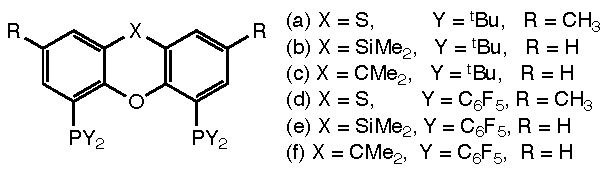
\includegraphics[]{../Figures/Proposedligands.pdf}
\caption[Proposed ligands for investigation]{Proposed ligands for investigation}
\label{Proposedligands}
\end{figure}

The coordination properties of the ligands will be investigated by formation of complexes with a range of metals including platinum, palladium, iridium and rhodium.  These late transition metals are electron-rich so will form weaker metal-oxygen bonds than the earlier and first row transition metals.  Halide complexes will be formed initially as the halide can be readily abstracted by a silver salt allowing the formation of three-coordinate complexes.  At this point the electronic properties of the complexes will be investigated by the formation of carbonyl complexes.  The carbonyl stretching frequency is commonly utilised as a measure of electron density on the metal.\cite{Tolman1977}  Measuring this frequency will allow a qualitative evaluation of the electron- withdrawing and donating properties of the ligands comparing the \emph{tert}-butyl and pentafluorophenyl ligands.  It was also be used to determine the electronic impact of altering the bridging group in the backbone between \ce{CMe2}, \ce{SiMe2} and S.  

Methyl complexes (Figure \ref{Methylcomplexes}) will be synthesised by treatment of the three-coordinate and halide complexes with a methylating agent such as dimethyl zinc or methyllithium. Investigation into the reactivity of methyl complexes with a variety of halogen and carbon based electrophiles to allow the formation of functionalised methane that could be readily converted into other compounds for use as chemical feedstocks or fuels.  
 
% including N-bromosuccinamide, bromine and methyl \emph{p}-toluenesulfonate.  Reaction with the bromine electrophiles will produce bromomethane, whilst reaction with \emph{p}-toluenesulfonate will form ethane which could be further converted \emph{via} alkane metathesis or dehydrogenation to yield the higher alkanes for use as fuels or ethene which is a useful organic starting material.  

\begin{figure}[h]  
\centering
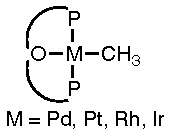
\includegraphics[]{../Figures/Methylcomplexes.pdf}
\caption[Methyl complexes]{Methyl complexes}
\label{Methylcomplexes}
\end{figure}

Further work will look at reactions of the synthesised metal complexes with alkanes focusing specifically on methane.  Upon complexation to a metal centre, the pK\sub{a} of methane decreases significantly so investigation into the reaction of various metal complexes with methane in the presence of strong bases will be carried out.  This should result in a methyl complex that can react with an appropriate electrophile \emph{in situ} to form a three-coordinate metal pincer complex and the resulting product.

Finally, the project will investigate the use of the pincer complexes for a one-pot catalytic synthesis of a useful chemical feedstock from methane.  This will involve combination of the C-H activation and electrophilic attack in the same step.

\section{Synthetic strategy}

\subsection{Ligand synthesis}

The commercially available carbon-bridged backbone will be utilised and the silicon- and sulfur-bridged backbones will be synthesised using literature methods for similar compounds.\cite{Kranenburg1995, Suter1938}  The ligands will be synthesised using a method derived from the literature for similar compounds.\cite{Kranenburg1995, Mispelaere2005}

The synthesis of the silicon bridged backbone (Scheme \ref{Siliconbackbone}) is based on that reported by Kranenburg et al.\cite{Kranenburg1995}  The synthesis involves lithiation of diphenylether at low temperature using \emph{n}-butyllithium and \gls{TMEDA} and warming to room temperature over 16 hours.  The reaction mixture is cooled to -78 \degrees C and a solution of dichlorodimethylsilane is added over one hour before stirring for 16 hours.  The reaction is quenched using water before isolation and recrystallisation from methanol.

\begin{scheme}[h]  
\centering
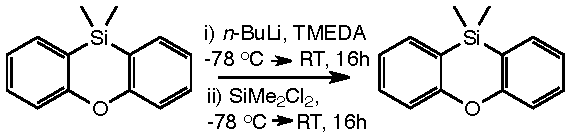
\includegraphics[]{../Schemes/Siliconbackbone.pdf}
\caption[Synthesis of the silicon bridged backbone]{Synthesis of the silicon bridged backbone}
\label{Siliconbackbone}
\end{scheme}

The sulfur bridged backbone will be synthesised by a Friedel-Crafts reaction (Scheme \ref{Sulfurbackbone}).\cite{Suter1938}  Anhydrous aluminium trichloride and sulfur are added to \emph{p}-ditolylether and heated to reflux for four hours.  The reaction is quenched with hydrochloric acid and washed with water.  The product is isolated from excess \emph{p}-ditolylether \emph{via} distillation under reduced pressure.

\begin{scheme}[h]  
\centering
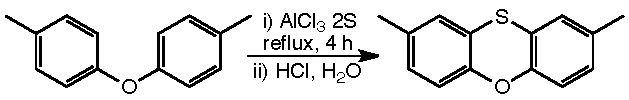
\includegraphics[]{../Schemes/Sulfurbackbone.pdf}
\caption[Synthesis of the sulfur-bridged backbone]{Synthesis of the sulfur-bridged backbone}
\label{Sulfurbackbone}
\end{scheme}

The chlorodi(pentafluorophenyl) phosphine and phosphine utilised in the ligand synthesis will be prepared as reported by Mancino et al. (Scheme \ref{Pentafluorophenyl}).\cite{Mancino2005}  The commercially available bromopentafluorobenzene will be treated with magnesium to yield a Grignard reagent.  Reaction of \ce{PCl3} with two equivalents of the Grignard reagent will yield the desired chlorodi(pentafluorophenyl) phosphine.   A similar method is already used within the research group for the synthesis of chlorodi(\emph{tert}-butyl) phosphine.

\begin{scheme}[h]  
\centering
\includegraphics[width = 0.8\textwidth]{../Schemes/Pentafluorophenyl2.pdf}
\caption[Synthesis of chlorodi(pentafluorophenyl) phosphine]{Synthesis of chlorodi(pentafluorophenyl) phosphine}
\label{Pentafluorophenyl}
\end{scheme}

The synthesis of the ligands from the backbones will be the same in all cases (Scheme \ref{tBuligandsynthesis}).  The method utilised is based on combination of the reported synthesis of xantphos and the bis-(\emph{tert}-butyl-phosphino) derivative of xantphos.\cite{Kranenburg1995, Mispelaere2005}  A solution of the precusor and \gls{TMEDA} in diethyl ether will be cooled to -78 \degrees C and treated with \emph{sec}-butyllithium before warming to room temperature over 16 hours.  Upon cooling to -78 \degrees C a solution of the appropriate phosphine in diethyl ether will be added dropwise and the reaction allowed to warm to room temperature over 16 hours.  The solution will be quenched by washing with water and the product recrystallised from \emph{n}-propanol.  

\begin{scheme}[h]  
\centering
\includegraphics[]{../Schemes/tBuligandsynthesis.pdf}
\caption[Synthesis of the ligands]{Synthesis of the ligands}
\label{tBuligandsynthesis}
\end{scheme}

\subsection{Coordination complexes}

Investigations into the coordination complexes formed with the proposed ligands will focus on late second and third row transition metals, namely platinum, palladium, iridium and rhodium.  These late transition metals will form weak bonds to the oxygen centre allowing for the weakly binding methane to bond in the \emph{trans}-position.  Reactions will be carried out with metal starting materials with weakly bound ligands that can be readily replaced by the desired ligands.  As xantphos typically forms bidentate complexes, \cite{Freixa2008} it is expected that a mixture of \emph{cis} and \emph{trans} bidentate complexes will be formed initially upon reaction of the ligand with a metal halide complex (Scheme \ref{Metalcomplexes} (a)).

\begin{scheme}[h]  
\centering
\includegraphics[]{../Schemes/Metalcomplexes.pdf}
\caption[Synthesis of the three-coordinate complexes]{Synthesis of the three coordinate complexes}
\label{Metalcomplexes}
\end{scheme}
\vspace{1cm}

Treatment of the bidentate metal halide complex with an appropriate ligand abstraction agent to remove the halide ligands will be required to promote tridentate coordination of the POP ligand.  Hence the halide complexes will be synthesised initially, as these can be treated with one or two equivalents of an appropriate silver salt, such as silver hexafluoroantimonate,  to yield the pincer coordination complex with either zero or one other ligand (Scheme \ref{Metalcomplexes} (b)).  The hexafluoroantimonate is a non-coordinating counterion so will not bond to the metal centre allowing the formation of the three-coordinate complex.  Halide abstraction under an atmosphere of carbon monoxide will allow the formation of the carbonyl complex (scheme \ref{Metalcomplexes} (c)), which will be studied using infrared spectroscopy to investigate the electronic influence of the different ligand systems.  

Upon formation of the three-coordinate complexes, treatment with a methylating agent such as dimethylzinc, methylmagnesium iodide or methyllithium will be carried out to obtain the methyl complexes (Scheme \ref{Metalcomplexes} (d)).  These complexes will be investigated for the reactive properties with a variety of electrophiles including \ce{Br2}, \emph{N}-bromosuccinamide, methyl \emph{p}-toluene sulfonate and methyl iodide.  The protonation of these complexes using acids with weakly coordinating counterions (\ce{(CF3SO2)2CHPh} and \ce{(CF3SO2)2CH2}) will be carried out in order to form $\sigma$-methane complexes which will be used to investigate the nature of the bond between the methane and the metal centre.  

Formation of the methyl complexes will also be attempted by reaction of the three-coordinate complexes with methane in the presence of a strong base (Scheme \ref{Metalcomplexes} (d)).  Upon complexation of methane, the pKa is expected to decrease similar to that found upon complexation of molecular hydrogen making deprotonation feasible.\cite{Crabtree1995}

%These methyl complexes will be reacted with a range of electrophiles to yield \fixme{bromomethane} which could be utilised as a useful chemical feedstock.

The final section of the project will investigate a combination of the C-H activation of methane to give the methyl complexes and their \emph{in situ} reaction with the electrophiles studied previously.  This will form a novel catalytic process for the formation of a useful chemical feedstock from methane.  

\section{Methodology and techniques}

All reactions will be carried out using Schlenk techniques under an inert atmosphere.  The resulting products will be characterised initially using NMR spectroscopy.  In particular \proton, \carbon~and \phosphorus~NMR, together with COSY, HSQC and HMBC experiments will be used to confirm the structural identity of the compounds.  Platinum and rhodium particularly useful as the spin 1/2, NMR active nucleus \Pt~and \ce{^{103}Rh} are 33\% and 100\% abundant.  This results in coupling of other active nuclei to the platinum, forming platinum satellites that can be used to obtain useful information about the complex.

Infrared spectroscopy will be particularly important to this project.  As oxygen NMR is not practicable, infrared spectroscopy will be utilised to distinguish between the bidentate and tridentate binding modes of the ligands.  In particular, the C-O stretch of the backbone should be readily identifiable (1243 \percm~for free xantphos\cite{Kranenburg1995}) and if the oxygen is coordinating to the metal the stretching frequency is expected to shift to lower frequency compared to both the free ligand and bidentate coordination.  Further characterisation will be carried out utilising X-ray crystallography, mass spectrometry and elemental analysis as required.  

\section{Proposed timeline}

%12 months of enrolment will be completed at 15th August 2011.

The initial six months will focus on the synthesis of the ligands.  The sulfur-bridged \emph{tert}-butyl ligand has been successfully synthesised and the synthesis of the silicon-bridged analogue has been attempted with promising results, although further work on isolation and optimisation is required.  Initially, work will focus on completing the synthesis of the silicon bridged ligand and successful synthesis of the carbon bridged ligand expecting to be completed by the end of August.  After successful synthesis of the \emph{tert}-butyl ligands the synthesis of the electron-withdrawing, pentafluorophenyl ligands will be attempted.  It is expected that the ligand synthesis stage will be completed in November 2011.

The investigation into the halide complexes and the halide abstraction to form the three-coordinate complexes will be carried out concurrently with the synthesis of the ligands.  It is expected that the  ligands will be air-sensitive, so it is important to carry out reactions of the ligands as close to the time of synthesis as possible.  However the complexes that are formed are more likely to be air-stable, so reactions of these can be carried out at a later date.

Synthesis and analysis of the carbonyl complexes and investigation into the methylation of the three-coordinate species will be carried out in early 2012, followed by the electrophilic reactions and C-H activation of methane.  The research into the catalytic reactions will be performed in early 2013.  The proposed submission date is August 2013. 

\begin{table}[h]
\caption[Proposed timeline]{Proposed timeline}
\label{Timeline}
\begin{center}
    \begin{tabular}{l l l}
    \hline
Project component					& Beginning Date 	& Completion Date	\\ \hline
\emph{tert}-butyl ligand synthesis		& In progress		& August 2011		\\
pentaflurophenyl ligand synthesis		& September 2011	& November 2011	\\
Synthesis of halide complexes			& August 2011		& December 2011	\\
Synthesis of three-coordinate complexes	& August 2011		& December 2011	\\
Synthesis of carbonyl complexes		& January 2012	& February 2012	\\
Methylation 						& March 2012		& May 2012		\\
Electrophilic reactions				& June 2012		& August 2012		\\
C-H activation of methane			& September 2012	& November 2012	\\
Catalytic investigations				& December 2012 	& March 2013		\\
Writing thesis 						& April 2013		& August 2013		\\
    \hline
    \end{tabular}
    \end{center} 
    \end{table}

%Relationship between dihydrogen and methane see Shilov 1997 pg 2881\\

%Electron rich metal\\
%	Stronger pi donation into sigma* orbital\\
%	Results in decreased bond order and cleavage of the bond\\
%	Oxygen very weak ligand on Pt  so would promote formation of a stronger bond trans to it\\
	
%Moulton 1976\\
%	Di-t-butylphosphines promote hydride formation, internal C- or O-metallation and co-ordinative unsaturation, stabilse unusual valence states such as Ir(II) or unusual compounds such as Pt dihydrides\\
	
%Zhu 2008: see conclusion for the impact of trans influence on C-H activation\\

%Synthesis of ethane or ethene from methane
	
%	The poor activity of pincer complexes compared to complexes with monodentate phosphine suggests that phosphine loss or rearrangement may be necessary for beta-elimination by the alkyl hydride intermediate.\cite{Wang1996}
	
%Activation of the methane under basic conditions.  Upon complexation of hydrogen with metals the pKa is reduced from 35 to 0-15.\cite{Crabtree2001}  The pKa of methane is 40/56 depending on source (40 from Crabtree1995\cite{Crabtree1995} 56 from Bordwell1988\cite{Bordwell1988}) pKa of various compounds in DMSO is given in table \ref{pKatable}

%\begin{table}[h]
%\caption[pKa's of various compounds]{pKa's of various compounds}
%\label{pKatable}
%\begin{center}
    %\begin{tabular}{l l l l}
    %\hline
%Compound 			& pKa 	& Reference\\ \hline
%Hydrogen 			& 35 		& \cite{Crabtree2001}\\
%Complexed Hydrogen 	& 0 - 15	& \cite{Crabtree2001}\\
%Methane				& 40 / 56  	& \cite{Bordwell1988}\\
%Xanthene				& 30		& \cite{Bordwell1988}\\
%Thioxanthene			& 28.6	& \cite{Bordwell1988}\\
%$^t$BuLi				& 53		& \cite{Bordwell1988}\\
%KO$^t$Bu				& 18		& \cite{Bordwell1988}\\
%LDA					& 36		& \cite{Bordwell1988}\\
    %\hline
    %\end{tabular}
    %\end{center} 
    %\end{table}

%Reaction under argon to prevent competitive binding of nitrogen\\
%Activation of methane under fischer-porter bottle synthesis\\
%Methyl complex may be too stable to undergo functionalisation i.e. will the methyl have orbitals / electron
%density available to donate / be donated into\\
%Possibility of using a source of Cl+ to react with the complexed methyl to form \ce{CH3Cl}\\
%Or using \ce{Br2}? better than chlorine gas\\
%Issue that the product may be more reactive towards the complex\\
%\ce{CH3Cl} bp = -24.2 \degrees C so will be a gas at RT\\
%\ce{CH3Br} bp = 3.56 \degrees C\\
%\ce{CH4} bp = -161.6 \degrees C\\
%Methane boils much lower so could use dry ice/acetone trap to condense the product from excess methane and collect excess methane in liquid \ce{N2} trap\\
%Rather than using a base use a borane to form the boron compound which could then react somehow\\



%The proposed research will not involve any animal or human subjects or tissues nor is not expected to impact  people's privacy, rights or freedoms and as such ethics approval is not required.

%Schlenk working under argon rather than nitrogen to prevent competitive binding\\
%Fischer-porter bottles?\\
%NMR (1D, \proton, \carbon, \phosphorus, 2D, HSQC, HMBC etc)\\
%Platinum as an NMR active nuclei\\
%IR (C-O bond stretch changes on coordination)\\
%X-Ray crystallography\\
%Mass spec\\
%Elemental analysis\\


%%!TEX root = Thesis.tex

\chapter{The vuwthesis.cls File}
\label{ch:thesiscls}

OK, this is big file and I don't even pretend to understand all of it.  It is based upon the report class which is supplied with \LaTeX{} but it is heavily edited and expanded upon to do everything I needed for the thesis.  I will only focus upon the bits that are of any particular relevance.

\small\singlespacing
\begin{verbatim}
\NeedsTeXFormat{LaTeX2e}
\ProvidesClass{thesis}

\DeclareOption*{\PassOptionsToClass{\CurrentOption}{report}}
\ProcessOptions

\LoadClass{report}
\end{verbatim}

\normalsize\doublespacing
Some introductory stuff which we'll ignore.

\small\singlespacing
\begin{verbatim}
% conditionals for this class file
\RequirePackage{ifpdf}
% default language
\RequirePackage[english]{babel}
% glossary package
\RequirePackage[number=none,toc=true]{glossary}
% prevent T1 encoding error
\RequirePackage[T1]{fontenc}
% line spacing
\RequirePackage{setspace}
% page geometry
\RequirePackage{geometry}
\ifpdf
	% figures package [for pdflatex]
	\RequirePackage[pdftex]{graphicx}
\else
	% figures package [for latex]
	\RequirePackage[dvips]{graphicx}
\fi
% chemical formulas
\RequirePackage[version=3]{mhchem}
% numbered structures
\RequirePackage{chemcompounds}
% color support
\RequirePackage{color}
% row spanning in tables
\RequirePackage{multirow}
% ACS referencing
\RequirePackage[numbers,sort&compress,super]{natbib}
% times font
\RequirePackage{times}
% tables with footnotes
\RequirePackage{threeparttable}
% sideways tables
\RequirePackage{rotating}
% new floats and caption layout
\RequirePackage{caption}
% subfigures
\RequirePackage{subfigure}
% slanted greater/less than or equals to
\RequirePackage{amssymb}
% source code support
\RequirePackage{listings}
% modification of labels in schemes
\RequirePackage[floats=float]{chemscheme}
\ifpdf
	% eps to pdf conversion on the fly [for pdflatex]
	\RequirePackage{epstopdf}
	% hyperlinks [for pdflatex]
	\RequirePackage[pdftex]{hyperref}
\else
	% hyperlinks [for latex]
	\RequirePackage[dvips]{hyperref}
\fi
\end{verbatim}

\normalsize\doublespacing
This tells the compiler which packages are needed to compile this documents of this class.  Each of these has been added for a reason and with the possible exception of the listings package, you will likely need them all.  Depending on your version of \LaTeX{} this may or may not pose problems.  MiKTeX for Windows users shouldn't have any problems because the update mechanism is so good.  Linux users may have to manually upgrade to the latest versions of some of these packages on their own. For the epstopdf package to work, Windows users will need to add ``\verb$--$enable-write18'' to the command line options for pdflatex in the ``Define output profiles'' option of TeXnicCenter.

\small\singlespacing
\begin{verbatim}
% Add a \textsubscript command equivalent to \textsuperscript
% From subscript.sty code fragment on CTAN
\DeclareRobustCommand*\textsubscript[1]{%
  \@textsubscript{\selectfont#1}}
\def\@textsubscript#1{%
  {\m@th\ensuremath{_{\mbox{\fontsize\sf@size\z@#1}}}}}
\end{verbatim}

\normalsize\doublespacing
Believe it or not, \LaTeX{} does not include a textsubscript command to complement its textsuperscript command.  This adds one.

\small\singlespacing
\begin{verbatim}
\lstset{basicstyle=\footnotesize\ttfamily}
\lstset{breaklines=true,showstringspaces=false}
\lstset{tabsize=3,breakindent=15pt}
\lstset{numbers=left,numberstyle=\tiny,stepnumber=5,
   numbersep=5pt,firstnumber=1}
\lstloadlanguages{[Visual]C++,Matlab}
\end{verbatim}

\normalsize\doublespacing
Some basic settings for the listings package.

\small\singlespacing
\begin{verbatim}
% use a wider glossary than the default 0.6\linewidth
\descriptionwidth=0.8\linewidth
% stop the glossary from grouping alphabetically
\setglossary{delimT={\cr & \cr},gloskip={}}
\end{verbatim}

\normalsize\doublespacing
Set up the glossary package.

\small\singlespacing
\begin{verbatim}
\geometry{hmargin={4cm,2cm},vmargin={1.5cm,2cm}}
\setlength{\parindent}{0pt}
\setlength{\parskip}{14pt plus 2pt minus 1pt}
\end{verbatim}

\normalsize\doublespacing
Here is where we define our margins, indentation and paragraph skip distance.  To prevent indenting at all, the indent length is set to 0 points.

\small\singlespacing
\begin{verbatim}
\def\@biblabel#1{#1.}
\end{verbatim}

\normalsize\doublespacing
Change the default labelling of reference entries.

\small\singlespacing
\begin{verbatim}
\def\subject#1{\gdef\@subject{#1}}
\def\degree#1{\gdef\@degree{#1}}
\def\institution#1{\gdef\@institution{#1}}
\def\logo#1{\gdef\@logo{#1}}

\renewcommand\maketitle{\begin{titlepage}%
	\let\footnotesize\small
	\let\footnoterule\relax
	\let \footnote \thanks
	\begin{center}\begin{large}%
		{\ } \par
		\vspace{1.5cm}
		{\huge\bfseries\@title\par}%
		\vspace{2cm}
		{by\\ \@author}\par
		\vspace{0.08\textheight}
		\includegraphics[height=4cm]{\@logo}\par
		\vspace{0.06\textheight}
		{A thesis\\ submitted to \@institution\\
		 in fulfilment of the\\requirements for the degree of\\
		 \@degree\\in \@subject.\\ \vspace{2cm}
		 \@institution\\ \@date \par}%
	\end{large}\end{center}\par
\end{titlepage}
\setcounter{footnote}{0}%
\global\let\thanks\relax
\global\let\maketitle\relax
\global\let\@thanks\@empty
\global\let\@author\@empty
\global\let\@date\@empty
\global\let\@title\@empty
\global\let\title\relax
\global\let\author\relax
\global\let\date\relax
\global\let\and\relax
}
\end{verbatim}

\normalsize\doublespacing
This complicated beast makes our title page.  Depending on the length of the title of your thesis, you may need to jigger around with the vertical spacings between the title and the logo etc.

\small\singlespacing
\begin{verbatim}
\renewcommand{\@makechapterhead}[1]{
   {
      \normalfont \centering \bfseries \Large
      \ifnum \c@secnumdepth >\m@ne
         \begin{itshape}
            \@chapapp\space\thechapter\par
         \end{itshape}
      \fi
      #1\par
      \vspace{0.5cm}%
   }
}

\renewcommand{\@makeschapterhead}[1]{
   {
      \normalfont \centering \bfseries \Large
      #1\par
      \vspace{0.5cm}%
   }
}
\end{verbatim}

\normalsize\doublespacing
This redefines the chapter headings.

\small\singlespacing
\begin{verbatim}
\renewcommand{\contentsname}{Table of Contents}
\renewcommand{\bibname}{References}
\end{verbatim}

\normalsize\doublespacing
And this names the contents pages and the bibliography appropriately.

\small\singlespacing
\begin{verbatim}
% Redefine the default placement of figures and table as bp (not
% tbp). I like figures/tables etc only to occur AFTER they are
% mentioned in the text. Because the chemscheme package doesn't
% initialise the scheme environment's placement until after
% \begin{document}, the redefinition of the scheme's placement
% must occur in thesis.tex.
\floatplacement{figure}{bp}
\floatplacement{table}{bp}
\end{verbatim}

\normalsize\doublespacing
Hopefully the comment is self-explanatory.  Floats can be placed htbp (here, top, bottom or page).  The \LaTeX{} default of tp often leads to figures going at the top of the page on which they are first referenced (ie. before the text) which I disliked.

\small\singlespacing
\begin{verbatim}
\newfloat{structure}{hbp}{lox}[chapter]
\end{verbatim}

\normalsize\doublespacing
Sets up structure as a new float type.  Schemes are already added as a float by the chemscheme package.

\small\singlespacing
\begin{verbatim}
\captionsetup{labelfont=bf,labelsep=space,
   justification=centering}
\end{verbatim}

\normalsize\doublespacing
Redefines the caption layout so ``Figure x.y'' is in bold and the rest of the caption is not.

\small\singlespacing
\begin{verbatim}
% Shortcuts for dH, dC and dN
\newcommand{\dH}{$\delta$\textsubscript{H}~}
\newcommand{\dC}{$\delta$\textsubscript{C}~}
\newcommand{\dN}{$\delta$\textsubscript{N}~}

% Shortcuts for 1H, 13C and 15N
\newcommand{\proton}{\ce{^{1}H}}
\newcommand{\carbon}{\ce{^{13}C}}
\newcommand{\nitrogen}{\ce{^{15}N}}

% Shortcuts for H2 and H3
\newcommand{\Htwo}{H\textsubscript{2}}
\newcommand{\Hthree}{H\textsubscript{3}}

% Shortcut for 1JCH etc.
\newcommand{\oneJCH}{\mbox{\textsuperscript{1}
   \emph{J}\textsubscript{CH}}}
\newcommand{\oneJNH}{\mbox{\textsuperscript{1}
   \emph{J}\textsubscript{NH}}}
\newcommand{\oneJXH}{\mbox{\textsuperscript{1}
   \emph{J}\textsubscript{XH}}}

% Shortcuts for [M + H]+, [M + Na]+, [M + NH4]+,
% [M - H]-, [M - Na]- and [M - 2Na]2-
\newcommand{\MplusH}{\mbox{[M + H]\textsuperscript{+}}}
\newcommand{\MplusNa}{\mbox{[M + Na]\textsuperscript{+}}}
\newcommand{\MplusAmmonium}{\mbox{[M + \ce{NH4}]
   \textsuperscript{+}}}
\newcommand{\MminusH}{\mbox{[M $-$ H]$^{-}$}}
\newcommand{\MminusNa}{\mbox{[M $-$ Na]$^{-}$}}
\newcommand{\MminusNaNa}{\mbox{[M $-$ 2Na]
   \textsuperscript{2}$^{-}$}}

% Shortcuts for lambda max and nu max
\newcommand{\lambdamax}{\mbox{$\lambda$\textsubscript{max}}}
\newcommand{\numax}{\mbox{$\nu$\textsubscript{max}}}

% Shortcut for reciprocal centimetres
\newcommand{\percm}{\mbox{cm$^{-}$\textsuperscript{1}}}

% Shortcut for degrees C
\newcommand{\degC}{\mbox{$\,^\circ$C}}

% Shortcuts for ED50, IC50, LC50 and LD50
\newcommand{\EDfifty}{\mbox{ED\textsubscript{50}}}
\newcommand{\ICfifty}{\mbox{IC\textsubscript{50}}}
\newcommand{\LCfifty}{\mbox{LC\textsubscript{50}}}
\newcommand{\LDfifty}{\mbox{LD\textsubscript{50}}}
\end{verbatim}

\normalsize\doublespacing
Here are a whole pile of newly defined commands to save typing later and to try and ensure consistency throughout the document.  Note that the ``\small\verb$~$\normalsize'' symbol forces a space after the command.  If you require a space after the other commands, you should follow them with double braces.  For example, the command ``\small\verb$\dH$\normalsize'' produces ``\dH'' (note the space at the end).  The command ``\small\verb$\proton spectra$\normalsize'' produces ``\proton spectra'' while ``\small\verb$\proton{} spectra$\normalsize'' produces ``\proton{} spectra'' which is probably what you want.  The ``\small\verb$\degC$\normalsize'' command produces a half-space followed by the degrees Centigrade symbol so you can just use ``\small\verb$20\degC$\normalsize'' to produce ``20\degC''.

\small\singlespacing
\begin{verbatim}
% Try and limit hyphenation
\hyphenpenalty=5000
\tolerance=1000
\end{verbatim}

\normalsize\doublespacing
Some commands to try and avoid too much hyphenation.

\small\singlespacing
\begin{verbatim}
% Standard typesetting for fields
\newcommand{\field}[1]{\textbf{#1}}
% and values of database entries
\newcommand{\entry}[1]{\textit{#1}}
\end{verbatim}

\normalsize\doublespacing
New commands to simplify the field and entry terms in my database chapter.

\small\singlespacing
\begin{verbatim}
\newcommand{\approximately}{ca.}
\end{verbatim}

\normalsize\doublespacing
By defining a command for approximately, I could change all instances at once if I needed to.

\small\singlespacing
\begin{verbatim}
% Use a,b,c etc. for footnotes to avoid confusion with \cite
\renewcommand{\thefootnote}{$\fnsymbol{footnote}$}
\end{verbatim}

\normalsize\doublespacing
Change footnotes to letters by default.  Numbers are obviously ambiguous with citations.

\small\singlespacing
\begin{verbatim}
\newcommand{\fixme}[1]{\colorbox[rgb]{1,0.5,0}{\textbf{#1}}}

\endinput
\end{verbatim}
\normalsize\doublespacing
The fixme command can be used to highlight stuff you still need to fix up (eg. ``\small\verb$\fixme{Don't forget to reference}$\normalsize'' produces ``\fixme{Don't forget to reference}'').  You can change the colour of the box by tailoring the rgb numbers to your liking.  Note that text in the fixme environment won't wrap to fit lines so either keep your comments short or use multiple fixme environments.

And that concludes the vuwthesis.cls file.  Now we'll look at some specific examples of how to put it all into use.

%%!TEX root = Thesis.tex

\chapter{Putting It All Together}
\label{ch:examples}

\section{The Basics}

OK, there are plenty of \LaTeX{} tutorials available on the web so I'm not going to dwell on the simple things too much.  You are going to want to use Greek characters at some point though so you need to know about math mode.  Math mode text is enclosed within dollar signs.  It is worth pointing out that in math mode, your normal font is changed so you will want to use math mode only for characters that you can't produce normally.  Basically, this includes the Greek alphabet and a few symbols.  For example, ``\small\verb&$\delta$&\normalsize'' produces ``$\delta$''.  Note the difference between ``\small\verb&$\lambda_{max}$&\normalsize'' which produces ``$\lambda_{max}$'' and my command ``\small\verb$\lambdamax$\normalsize'' which produces ``\lambdamax''.  Trying to avoid font discrepancies was one of the main reasons behind defining all those extra commands.  Capital Greek letters are produced with the corresponding capitalised command (eg. ``\small\verb&$\Delta$&\normalsize'' produces ``$\Delta$'').

Another useful trick to know is that a tilde produces a non-breaking space.  It's particularly useful between measurements and units to prevent them from ever being split at the end of a line.  eg. ``\small\verb$12~cm$\normalsize'' or ``\small\verb$8.4~min$\normalsize''.

\section{Glossary Entries}
As I mentioned before, I like to keep all my glossary entries in one place so I keep them in glossaryentries.tex and include that file before the introduction in the main thesis.tex file.  The format for glossary entries is:

\small\singlespacing
\begin{verbatim}
\glossary{name,description=high-resolution
   electrospray ionisation mass spectrometry}
\glossary{name=IPA,description=isopropyl alcohol}
\end{verbatim}

\normalsize\doublespacing
The output from the two commands above can be found on the glossary page.  If you're not getting a glossary page when you compile, take note of the instructions in Chapter \ref{ch:compiling} and make sure that you are running makeglos.pl or makeindex correctly.

\section{Compounds}

One of the coolest things about \LaTeX{} is its ability to automatically number everything.  Every time you use a ``\small\verb$\chapter{...}$\normalsize'' or ``\small\verb$\section{...}$\normalsize'' command, it gets added to the table of contents.  The chemcompounds package adds support for automatic numbering of compounds.  Whenever you want to refer to the number of a compound, you simply use ``\small\verb$\compound{compoundname}$\normalsize''.  The first time compoundname is encountered, it gets assigned a number.  From there on in, subsequent references to it will use the old number.  For example,\\
``\small\verb$Compound A (\compound{cpdA}) is similar to compound B$\\
\verb$(\compound{cpdB}).$\normalsize''\\
produces ``Compound A (\compound{cpdA}) is similar to compound B (\compound{cpdB}).''

OK, what about if we have three compounds and want to list 2--4?  We need to tell \LaTeX{} that compound 3 exists, but we don't want to actually print the number 3.  The following will achieve that:\\
``\small\verb$Compounds B--D (\compound{cpdB}--\compound*{cpdC}$\\
\verb$\compound{cpdD}) \ldots$\normalsize''\\
outputs ``Compounds B--D (\compound{cpdB}--\compound*{cpdC}\compound{cpdD}) \ldots''.

Two things to note -- the \small\verb$--$\normalsize{} command produces a longer dash than a single dash which should only be used in double-barrelled words.  The ``\small\verb$\ldots$\normalsize'' command produces ellipses which look better than ``...''.

Typos are your enemy here -- if you type the name of the identifier wrong, then it will get a new number!

\section{Figures and Schemes}

Here is some basic code for a figure:

\begin{verbatim}
\begin{figure}
\centerline{\includegraphics[width=0.5\textwidth]
    {figures/dictyodendrilladendyi}}
\caption{\emph{Dictyodendrilla dendyi}.}
\label{fig:dictyodendrilladendyi}
\end{figure}
\end{verbatim}

First, we begin a figure environment. Next, we include the figure ``dictyodendrilladendyi'' from the figures directory.  It should be a jpg, png or pdf file for pdflatex or an eps file for latex -- in this case, a png.  Setting the width of the picture to ``\small\verb$0.5\textwidth$\normalsize'' scales the picture to half the width of the area between the left and right margins of the page.  Everything enclosed in the centerline command is centered.

Then we include a caption.  The ``\small\verb$\emph{...}$\normalsize'' command italicises the contents.

Finally, we add a label.  This can be anything you like but it is useful to preface figures with ``fig:'', chapters with ``ch:'' etc. in case two things might otherwise have the same name.  The label is used later to refer to this figure.

\begin{figure}
\centerline{\includegraphics[width=0.5\textwidth]
    {figures/dictyodendrilladendyi}}
\caption{\emph{Dictyodendrilla dendyi}.}
\label{fig:dictyodendrilladendyi}
\end{figure}

Schemes are handled identically to figures.  The only difference between them as far as \LaTeX{} is concerned is that two separate numbering schemes are maintained.  The following inserts a scheme using the full width of the page:

\begin{verbatim}
\begin{scheme}
\centerline{\includegraphics[width=\textwidth]
   {schemes/tyrosineBuildingBlocks}}
\caption{Formation of tyramine and
   3-(4-hydroxyphenyl)pyruvate.}
\label{sch:tyrosineBuildingBlocks}
\end{scheme}
\end{verbatim}

In this case the included file is actually a pdf.  I found the best way to include anything from ChemDraw was to save it from ChemDraw as both a cdx master copy and an eps. The epstopdf package will then convert the eps to a pdf on the fly at compile time. If you are using MiKTeX and TeXnicCenter under Windows, then you will need to add ``\verb$--$enable-write18'' to the command line options for pdflatex in the ``Define output profiles'' option of TeXnicCenter for the eps to pdf conversion to work. If you are using latex then it will just use the eps file.

It is possible to direct the placement of a float by placing the letters hbtp (here, bottom, top, page) in square brackets after the ``\small\verb$\begin$\normalsize'' command. For example, ``\small\verb$\begin{scheme}[btp]$\normalsize'' instructs \LaTeX to try and place the scheme at the bottom of the current page, the top of the next page or on a page of its own in that order. I \textbf{strongly} recommend not overriding the default float placements until a given chapter is completely finished.

\begin{scheme}
\centerline{\includegraphics[width=\textwidth]
   {schemes/tyrosineBuildingBlocks}}
\caption{Formation of tyramine and 3-(4-hydroxyphenyl)pyruvate.}
\label{sch:tyrosineBuildingBlocks}
\end{scheme}

\section{Structures}
We insert a structure as follows:

\begin{verbatim}
\begin{structure}
\centerline{\includegraphics{structures/petrosynol}}
\centerline{\compound{petrosynol}}
\end{structure}
\end{verbatim}

We simply start a structure environment, include our graphics (centered of course) and then on the line below, include the compound number.  Later I will detail how to include multiple structures on a line and/or include tables of similar structures.

\begin{structure}
\centerline{\includegraphics{structures/petrosynol}}
\centerline{\compound{petrosynol}}
\end{structure}

\section{Tables}

\small\singlespacing
\begin{verbatim}
\begin{table}
\caption[Taxonomic classification of genus \emph{Petrosia}
  from order Haplosclerida.]{Taxonomic classification of
  genus \emph{Petrosia} from order Haplosclerida as presented
  by Hooper and van Soest.\cite{1}}
\end{verbatim}

\normalsize\doublespacing
Here is a table directly from my thesis.  There is a LOT of stuff here so I've broken it up, but it's all useful.  First, since captions go above tables, we start with the caption.  You'll note that I have the title twice - the first, enclosed in square braces will appear in the table of contents.  The second appears above the table.  In this case, this was done to prevent the reference to Hooper and van Soest from appearing in the contents.

\small\singlespacing
\begin{verbatim}
\label{tab:petrosia}
\begin{center}
\footnotesize
\begin{tabular}{l|l|l|l}
\end{verbatim}

\normalsize\doublespacing
A label is assigned to refer to later.  We then begin a center environment.  We switch to footnotesize (which is smaller than small, but larger than scriptsize and tiny) and begin a tabular environment with four left-aligned columns.

\small\singlespacing
\begin{verbatim}
Order & Sub-order & Family & Genus \\
\hline
\hline
\end{verbatim}

\normalsize\doublespacing
A simple header line.  Each cell is separated by an ``\small\verb$&$\normalsize`` and the row is terminated by ``\small\verb$\\$\normalsize``.  The ''\small\verb$\hline$\normalsize'' command inserts a horizontal line the full with of the table.  Using it twice inserts a double-line.

\small\singlespacing
\begin{verbatim}
\multirow{15}{*}{\color{blue}Haplosclerida} &
   \multirow{3}{*}{Haplosclerina} & Callyspongiidae
   & \ldots \\
\cline{3-4}
\end{verbatim}

\normalsize\doublespacing
Now we get a little more complicated.  The text ``Haplosclerida'' is centered down the first column over 15 rows.  The asterisk indicates that the column should be automatically sized to fit the text.  Note how to make the text blue using the ``\small\verb$\color{blue}$\normalsize`` command.  The ''\small\verb$\cline{3-4}$\normalsize`` command prints a horizontal line between columns 3 and 4 only.

\small\singlespacing
\begin{verbatim}
 & & Chalinidae & \ldots \\
\cline{3-4}
...
 & & Spongillidae & \ldots \\
\hline
\end{verbatim}

\normalsize\doublespacing
The rest of the table should be pretty self explanatory.  Empty cells are indicated by leaving a blank between the ampersands.

\small\singlespacing
\begin{verbatim}
\end{tabular}
\end{center}
\end{table}
\end{verbatim}

\normalsize\doublespacing
Finally, we end the tabular, center and table environments and we're done.  It looks like this:

\begin{table}[t]
\caption[Taxonomic classification of genus \emph{Petrosia} from order Haplosclerida.]{Taxonomic classification of genus \emph{Petrosia} from order Haplosclerida as presented by Hooper and van Soest.\cite{1}}
\label{tab:petrosia}
\begin{center}
\footnotesize
\begin{tabular}{l|l|l|l}
Order & Sub-order & Family & Genus \\
\hline
\hline
\multirow{15}{*}{\color{blue}Haplosclerida} & \multirow{3}{*}{Haplosclerina} & Callyspongiidae & \ldots \\ 
\cline{3-4}
 & & Chalinidae & \ldots \\
\cline{3-4}
 & & Niphatidae & \ldots \\
\cline{2-4}
 & \multirow{6}{*}{\color{blue}Petrosina} & Calcifibrospongiidae & \ldots \\
\cline{3-4}
 & & \multirow{4}{*}{\color{blue}Petrosiidae} & \emph{Acanthostrongylophora} \\
\cline{4-4}
 & & & \emph{Neopetrosia} \\
\cline{4-4}
 & & & \color{blue}\emph{Petrosia} \\
\cline{4-4}
 & & & \emph{Xestospongia} \\
\cline{3-4}
 & & Phloeodyctyidae & \ldots \\
\cline{2-4}
 & \multirow{6}{*}{Spongilina} & Lubomirskiidae & \ldots \\
\cline{3-4}
 & & Malawispongiidae & \ldots \\
\cline{3-4}
 & & Metaniidae & \ldots \\
\cline{3-4}
 & & Metschnikowiidae & \ldots \\
\cline{3-4}
 & & Potamolepidae & \ldots \\
\cline{3-4}
 & & Spongillidae & \ldots \\
\hline
\end{tabular}
\end{center}
\end{table}

\section{Combinations}

OK, now here are some examples of the more complicated things you can do with embedded tables/figures/structures etc.  Of particular use is the minipage environment which can break one section of page into several smaller pseudo-pages.

Here is an example of layout out three structures in one line, one of which has two R groups and therefore uses a table to list the compound names.

\small\singlespacing
\begin{verbatim}
\begin{structure}
\centering
\begin{minipage}[c]{0.33\textwidth}
\centerline{\includegraphics
   {structures/bromomethylhexacosadienoicAcids}}
\centerline{\begin{tabular}{lll}
\compound{cpdA} & \ce{R1} = H & \ce{R2} = Me \\
\compound{cpdB} & \ce{R1} = Me & \ce{R2} = H \\
\end{tabular}}
\end{minipage}%
\end{verbatim}

\normalsize\doublespacing
First, we begin a structure environment to contain all three structures then we turn on centering.  Next, we start a minipage environment which is one third of the textwidth wide, the contents of which should be centered.  Then we include the picture of the structure.  Next, we start a tabular environment with three left-aligned columns.  We fill in the details of the table as for a normal table.  Note the ``\small\verb$\ce{...}$\normalsize'' environment lays out chemical formulae.  Finally, we end the tabular and minipage environments.  Take note of the percent sign at the end of the block -- this ensures that there is no gap left between this minipage and the next one we are about to open.  Since we will create three minipages, each one third of the page wide, any spaces will cause the third minipage to line-wrap.

\small\singlespacing
\begin{verbatim}
\begin{minipage}[c]{0.34\textwidth}
\centerline{\includegraphics
   {structures/triacontadienoicAcid}}
\centerline{\compound{cpdC}}
\end{minipage}%
\end{verbatim}

\normalsize\doublespacing
The second structure is pretty self-explanatory -- again, we need the percent sign at the end.

\small\singlespacing
\begin{verbatim}
\begin{minipage}[c]{0.33\textwidth}
\centerline{\includegraphics
   {structures/tetratriacontapentaenoicAcid}}
\centerline{\compound{cpdD}}
\end{minipage}%
\end{structure}
\end{verbatim}

\normalsize\doublespacing
And ditto with the third.  Finally, we end the structure environment.  The output is:

\begin{structure}
\centering
\begin{minipage}[c]{0.33\textwidth}
\centerline{\includegraphics{structures/bromomethylhexacosadienoicAcids}}
\centerline{\begin{tabular}{lll}
\compound{cpdA} & \ce{R1} = H & \ce{R2} = Me \\
\compound{cpdB} & \ce{R1} = Me & \ce{R2} = H \\
\end{tabular}}
\end{minipage}%
\begin{minipage}[c]{0.34\textwidth}
\centerline{\includegraphics{structures/triacontadienoicAcid}}
\centerline{\compound{cpdC}}
\end{minipage}%
\begin{minipage}[c]{0.33\textwidth}
\centerline{\includegraphics{structures/tetratriacontapentaenoicAcid}}
\centerline{\compound{cpdD}}
\end{minipage}%
\end{structure}

As a final example, here is one of the most complicated tables I had to put together in my thesis -- the compiled NMR data for dictyodendrin F (\compound{dictyodendrinF}).

\small\singlespacing
\begin{verbatim}
\begin{sidewaystable}
\caption[NMR data (d\textsubscript{6}-DMSO) for
   dictyodendrin~F.]{\nitrogen{} (60~MHz), \carbon{}
   (125~MHz) and \proton{} (600~MHz) NMR data
   (d\textsubscript{6}-DMSO) for dictyodendrin~F
   (\compound{dictyodendrinF}).}
\label{tab:dictyodendrinFNMRDMSO}
\begin{center}
\begin{threeparttable}[c]
\scriptsize
\begin{tabular}{c c ccc c ccc ccc}
\cline{2-12}
\rule{0pt}{2.2ex} & & \multicolumn{3}{c}{\carbon{} or
   \nitrogen{}} & & \multicolumn{3}{c}{\proton{}} &
   & HMBC & \\
\cline{3-5}\cline{7-9}
\rule{0pt}{2.2ex} & Position & $\delta$~(ppm) & mult &
   \oneJXH{}~(Hz) & & $\delta$~(ppm) & mult &
   \emph{J}~(Hz) & COSY & (\proton{} to \carbon{} or
   \nitrogen{}) & NOE\\
\cline{2-12}
\multirow{34}{*}{
\begin{tabular}{c}
\includegraphics{structures/dictyodendrinF}\\
\normalsize\compound{dictyodendrinF}\\
\end{tabular}
} & 1 & $-$247.6 & s & & & & & & & & \\
& 2 & 170.6 & s & & & & & & & & \\
& 3 & 127.9 & s & & & & & & & & \\
& 4 & 133.3\tnote{\dag} & s & & & & & & & & \\
& 5 & 111.8 & s & & & & & & & & \\
& 6 & 124.7 & s & & & & & & & & \\
& 7 & 114.2 & d & 172 & & 5.74 & dd & 7.8, 1.3 &
   8,9 & 5,6,9,10,11 & 8,9,32,33\\
& 8 & 121.9 & d & 156 & & 6.59 & t & 7.6 & 7,9 &
   6,7,9,10,11 & 7\\
& 9 & 109.1 & d & 160 & & 6.56 & dd & 7.6, 1.4 &
   7,8 & 7,10,11,12 & 7\\
& 10 & 144.5 & s & & & & & & & & \\
& 11 & 128.7 & s & & & & & & & & \\
& 12 & $-$249.7 & d & \tnote{*} & & & & & & & \\
& 13 & 131.7\tnote{\dag} & s & & & & & & & & \\
& 14 & 178.3\tnote{\dag} & s & & & & & & & & \\
& 15 & 117.2 & s & & & & & & & & \\
& 16 & 148.0 & s & & & & & & & & \\
& 17 & 121.8\tnote{\ddag} & s & & & & & & & & \\
& 18[22] & 132.4 & d & 168 & & 7.23 & d & 8.3 &
   19 & 15,19,20,22 & 19,23,24\\
& 19[21] & 114.7 & d & 160 & & 6.88 & d & 8.6 &
   18 & 17,20,21 & 18,23,24\\
& 20 & 157.5 & s & & & & & & & & \\
& 23 & 42.4 & t & 141 & & 3.30 & t & 8.2 & 24 &
   2,16,24,25 & 18,19,24,26\\
& 24 & 33.2 & t & 130 & & 2.30 & t & 8.0 & 23 &
   1,23,25,26 & 18,19,23,26\\
& 25 & 127.8 & s & & & & & & & & \\
& 26[30] & 129.3 & d & 168 & & 6.56 & d & 8.8
   & 27 & 24,28,30 & 23,24\\
& 27[29] & 114.9 & d & 160 & & 6.54 & d & 8.8
   & 26 & 25,26,28,29 & \\
& 28 & 155.6 & s & & & & & & & & \\
& 31 & 122.3\tnote{\ddag} & s & & & & & & & & \\
& 32[36] & 132.0 & d & 164 & & 7.28 & d & 8.6 &
   33 & 3,33,34,36 & 7,33\\
& 33[35] & 115.0 & d & 160 & & 6.88 & d & 8.6 & \\
   32 & 31,34,35 & 7,32\\
& 34 & 158.5 & s & & & & & & & & \\
& OH & & & & & 9.15 & br s & & & & \\
& OH & & & & & 9.70 & br s & & & & \\
& OH & & & & & 9.90 & br s & & & & \\
& OH & & & & & 12.04 & br s & & & & \\
\cline{2-12}
\end{tabular}
\begin{tablenotes}
\item{\dag}{Tentatively assigned by comparison to
   the \ce{CD3OH} data.}
\item{\ddag}{Assignment interchangeable.}
\item{*}{Unable to be determined.}
\end{tablenotes}
\end{threeparttable}
\end{center}
\end{sidewaystable}
\end{verbatim}

\normalsize\doublespacing
I won't go into all the details -- most of it should be fairly self-explanatory by now (I hope).  You'll note however that this table makes uses ''sidewaystable`` instead of just ''table``.  It also uses the ''threeparttable`` package to allow the use of footnotes within the table.  If you can work your way through this example and understand what is going on, then you're standing in good stead.

\begin{sidewaystable}
\caption[NMR data (d\textsubscript{6}-DMSO) for dictyodendrin~F.]{\nitrogen{} (60~MHz), \carbon{} (125~MHz) and \proton{} (600~MHz) NMR data (d\textsubscript{6}-DMSO) for dictyodendrin~F (\compound{dictyodendrinF}).}
\label{tab:dictyodendrinFNMRDMSO}
\begin{center}
\begin{threeparttable}[c]
\scriptsize
\begin{tabular}{c c ccc c ccc ccc}
\cline{2-12}
\rule{0pt}{2.2ex} & & \multicolumn{3}{c}{\carbon{} or \nitrogen{}} & & \multicolumn{3}{c}{\proton{}} & & HMBC & \\
\cline{3-5}\cline{7-9}
\rule{0pt}{2.2ex} & Position & $\delta$~(ppm) & mult & \oneJXH{}~(Hz) & & $\delta$~(ppm) & mult & \emph{J}~(Hz) & COSY & (\proton{} to \carbon{} or \nitrogen{}) & NOE\\
\cline{2-12}
\multirow{34}{*}{
\begin{tabular}{c}
\includegraphics{structures/dictyodendrinF}\\
\normalsize\compound{dictyodendrinF}\\
\end{tabular}
} & 1 & $-$247.6 & s & & & & & & & & \\
& 2 & 170.6 & s & & & & & & & & \\
& 3 & 127.9 & s & & & & & & & & \\
& 4 & 133.3\tnote{\dag} & s & & & & & & & & \\
& 5 & 111.8 & s & & & & & & & & \\
& 6 & 124.7 & s & & & & & & & & \\
& 7 & 114.2 & d & 172 & & 5.74 & dd & 7.8, 1.3 & 8,9 & 5,6,9,10,11 & 8,9,32,33\\
& 8 & 121.9 & d & 156 & & 6.59 & t & 7.6 & 7,9 & 6,7,9,10,11 & 7\\
& 9 & 109.1 & d & 160 & & 6.56 & dd & 7.6, 1.4 & 7,8 & 7,10,11,12 & 7\\
& 10 & 144.5 & s & & & & & & & & \\
& 11 & 128.7 & s & & & & & & & & \\
& 12 & $-$249.7 & d & \tnote{*} & & & & & & & \\
& 13 & 131.7\tnote{\dag} & s & & & & & & & & \\
& 14 & 178.3\tnote{\dag} & s & & & & & & & & \\
& 15 & 117.2 & s & & & & & & & & \\
& 16 & 148.0 & s & & & & & & & & \\
& 17 & 121.8\tnote{\ddag} & s & & & & & & & & \\
& 18[22] & 132.4 & d & 168 & & 7.23 & d & 8.3 & 19 & 15,19,20,22 & 19,23,24\\
& 19[21] & 114.7 & d & 160 & & 6.88 & d & 8.6 & 18 & 17,20,21 & 18,23,24\\
& 20 & 157.5 & s & & & & & & & & \\
& 23 & 42.4 & t & 141 & & 3.30 & t & 8.2 & 24 & 2,16,24,25 & 18,19,24,26\\
& 24 & 33.2 & t & 130 & & 2.30 & t & 8.0 & 23 & 1,23,25,26 & 18,19,23,26\\
& 25 & 127.8 & s & & & & & & & & \\
& 26[30] & 129.3 & d & 168 & & 6.56 & d & 8.8 & 27 & 24,28,30 & 23,24\\
& 27[29] & 114.9 & d & 160 & & 6.54 & d & 8.8 & 26 & 25,26,28,29 & \\
& 28 & 155.6 & s & & & & & & & & \\
& 31 & 122.3\tnote{\ddag} & s & & & & & & & & \\
& 32[36] & 132.0 & d & 164 & & 7.28 & d & 8.6 & 33 & 3,33,34,36 & 7,33\\
& 33[35] & 115.0 & d & 160 & & 6.88 & d & 8.6 & 32 & 31,34,35 & 7,32\\
& 34 & 158.5 & s & & & & & & & & \\
& OH & & & & & 9.15 & br s & & & & \\
& OH & & & & & 9.70 & br s & & & & \\
& OH & & & & & 9.90 & br s & & & & \\
& OH & & & & & 12.04 & br s & & & & \\
\cline{2-12}
\end{tabular}
\begin{tablenotes}
\item{\dag}{Tentatively assigned by comparison to the \ce{CD3OH} data.}
\item{\ddag}{Assignment interchangeable.}
\item{*}{Unable to be determined.}
\end{tablenotes}
\end{threeparttable}
\end{center}
\end{sidewaystable}

\section{Referencing}

If we want to refer to say the picture of \emph{Dictyodendrilla dendyi} then we can use the label we attached to it earlier.  For example, ``See Figure \ref{fig:dictyodendrilladendyi}'' is produced by:\\
``\small\verb$See Figure \ref{fig:dictyodendtilladendyi}$\normalsize''

As you saw in the Petrosia table, citations are made with the ``\small\verb$\cite{num}$\normalsize'' command where ``num'' is the relevant entry (or comma-separated list of entries) in the thesis.bib file.

Thus, I can cite the last five years of NPR reviews\cite{2,3,4,5,6,7} with ``\small\verb$\cite{2,3,4,5,6,7}$\normalsize''.

\section{The chemscheme Package}

I did not need this package for my thesis so I am less familiar with the details.  However, using this package it is possible to place \LaTeX numbers within chemdraw schemes which are saved as eps documents.  This only works if you use latex to compile your document to a dvi and then convert the document to a pdf with dvipdf or a similar utility.  This will not work at all using pdflatex directly.

In this example, benzene (\compound{benzene}) is acylated via a Friedel-Crafts acylation with benzoyl chloride to form benzophenone (\compound{benzophenone}).

\begin{scheme}[hb]
\centerline{\includegraphics{schemes/numberedScheme}}
\caption{A numbered scheme without modification.}
\label{sch:numberedScheme}
\end{scheme}

\begin{scheme}[hb]
\schemeref[TMP1]{benzene}
\schemeref[TMP2]{benzophenone}
\centerline{\includegraphics{schemes/numberedScheme}}
\caption{A numbered scheme with modification.}
\label{sch:numberedSchemeModified}
\end{scheme}

The code to achieve the second example is as follows (the first is identical but missing the ''\small\verb$\schemeref$\normalsize'' commands):

\small\singlespacing
\begin{verbatim}
\begin{scheme}[hb]
\schemeref[TMP1]{benzene}
\schemeref[TMP2]{benzophenone}
\centerline{\includegraphics{schemes/numberedScheme}}
\caption{A numbered scheme with modification.}
\label{sch:numberedSchemeModified}
\end{scheme}
\end{verbatim}

\normalsize\doublespacing
As you can see, the text ``TMP1'' and ``TMP2'' in the chemdraw eps file is replaced with the compound numbers for benzene and benzophenone respectively.
%%!TEX root = Thesis.tex

\chapter{Compiling the Document}
\label{ch:compiling}

OK, finally to make your document, you're going to need to run the following commands:

\small\singlespacing
\begin{verbatim}
pdflatex thesis
bibtex thesis
pdflatex thesis
bibtex thesis
makeglos.pl thesis
pdflatex thesis
pdflatex thesis
\end{verbatim}

\normalsize\doublespacing
or

\small\singlespacing
\begin{verbatim}
pdflatex thesis
bibtex thesis
pdflatex thesis
bibtex thesis
makeindex -s thesis.ist -t thesis.glg -o thesis.gls thesis.glo
pdflatex thesis
pdflatex thesis
\end{verbatim}

\normalsize\doublespacing

If you are using Kile or MiKTeX, most of this will be done automatically.  However, you should ensure that BibTeX and makeindex processing are enabled for your project.  In MiKTeX, you can set the makeindex parameters to the following to achieve the required results:

-s ``\%bm''.ist -t ``\%bm''.glg -o ``\%bm''.gls ``\%bm''.glo

In Linux, it is easier to use the provided makeglos.pl perl script.

Note that ``pdflatex'' is run several times (perhaps more than is strictly necessary) in order to ensure that all cross-referencing is correct.

If you are using latex instead of pdflatex, simply substitute ``latex'' for ``pdflatex''. 

%%!TEX root = Thesis.tex

\chapter{Conclusion}
\label{ch:conclusion}

So there you have it.  The only thing left is the appendix in which you may want to include spectra.  The code for how I did it is as follows:

\small\singlespacing
\begin{verbatim}
\chapter{Raspailodane~F Spectra}
\label{app:raspailodaneFSpectra}

\begin{figure}[!hb]
\begin{flushright}
\includegraphics[height=0.75\textheight]
   {spectra/raspailodaneF1H}
\end{flushright}
\centerline{\proton{} NMR spectrum of raspailodane~F
   (\compound{raspailodaneF}) (300~MHz, \ce{CDCl3})}
\end{figure}

\begin{figure}[p]
\includegraphics[width=\textwidth]
   {spectra/raspailodaneFCOSY}
\centerline{COSY spectrum of raspailodane~F
   (\compound{raspailodaneF}) (300~MHz, \ce{CDCl3})}
\end{figure}

\begin{figure}[p]
\includegraphics[width=\textwidth]
   {spectra/raspailodaneFHSQC}
\centerline{HSQC spectrum of raspailodane~F
   (\compound{raspailodaneF}) (300~MHz, \ce{CDCl3})}
\end{figure}
\end{verbatim}

\normalsize\doublespacing
Hopefully by now most of that speaks for itself.  The flushright environment just right-aligns everything.  Note the [!hb] tag for the first spectrum -- it wouldn't stay on the same page as the title without the exclamation mark!  The others are all set to full-page images.

My last piece of advice -- I read once that \LaTeX{} treats every word/environment as a ``box''.  Words are boxes with stretchy space between them.  A minipage is just a box with more boxes in it.  If you use a command like ``\small\verb$\mbox{...}$\normalsize'' then the text is all contained in the one box which you will need to make sure isn't too big for your line since it no longer contains ``stretchy space''.

Included with this template is a copy of my thesis.  It is an online pdf version of the document so it includes coloured links and back-referencing which I have left out of the basic template.  If you want to know how I did that, or anything in particular which I may not have detailed here, please ask.

Best of luck.
%!TEX root = Thesis.tex

\chapter{Experimental}
\label{ch:expt}

\section{General procedures}
\label{section:generalprocedures}

\fixme{copied from Almas, check that the necessary info is here, everything is correct and everything unneccessary is removed}

All reactions and manipulation of products and reagents were carried out under an inert nitrogen atmosphere using standard Schlenk line techniques unless otherwise stated.  Analytical grade reagents and high purity solvents were degassed and purged with nitrogen before use, except for diethyl ether and tetrahydrofuran which were dried by refluxing over sodium/benzophenone ketyl.  NMR spectra were recorded using a Varian Unity Inova 300 (300~MHz for \proton, 75~MHz for \carbon, 121~MHz for \phosphorus{} and 282~MHz for \fluorine), a Varian Unity Inova 500 (500~MHz for \proton{} and 125~MHz for \carbon), or a Varian DirectDrive 600 (600~MHz for \proton, 150~MHz for \carbon{} and 60~MHz for \nitrogen) spectrometers.  The 600~MHz instrument was equipped with a Varian inverse-detected triple-resonance HCN cold probe operating at 25~K.  All direct-detected \proton{} and \carbon{} chemical shifts were referenced to the residual solvent peak.\cite{Fulmer2010}  NMR samples were prepared under an inert nitrogen or argon atmosphere unless otherwise stated, using \ce{C6D6}, \ce{CDCl3}, \ce{CD2Cl2}, acetone-\ce{d6} and toluene-\ce{d8}.  All NMR solvents were degassed before use and stored under inert atmosphere over molecular sieves.  Variable temperature NMR was carried out in toluene-\ce{d8} or \ce{CD2Cl2} using Varian Unity Inova 300~MHz NMR spectrometer.  Infrared spectra were recorded with a PerkinElmer Spectrum One FT-IR spectrophotometer using pressed KBr discs.  Microanalyses were performed by The Campbell Microanalytical Laboratory at Otago University.  Melting points were recorded on a Gallenkamp Melting Point Apparatus under vacuum unless otherwise stated. Single crystal \textit{X}-ray diffraction data were recorded by the \textit{X}-ray Crystallography Laboratory at the University of Canterbury.  Electrospray ionisation mass spectra were either recorded on a PE Biosystem Mariner 5158 TOF mass spectrometer at Victoria University, or performed by the GlycoSyn QC laboratory at Industrial Research Limited using a Waters Q-TOF Premier Tandem mass spectrometer.  Calculated \proton{} NMR spectra were obtained from gNMR spectral simulation programme, version 5.0.6.0 written by P. H. M. Budzelaar, IvorySoft 2006.

%\subsection*{Crystallography} 
%\label{subsec:X-ray}

%Diffraction data\footnote{Bruker {\scriptsize{SMART}} (Version 5.054), {\scriptsize{SADABS}} (Version 2.03), and {\scriptsize{SAINT}} (Version 6.02A), Bruker AXS Inc., Madison, Wisconsin, USA, 1997.} (see Tables \ref{tab:dataPN582}, \ref{tab:dataPdPNCl2}, \ref{tab:datanbagostic}, \ref{tab:datadimer} for details) were collected using Bruker CCD diffractometers with Mo K$\alpha$ radiation (0.71073~\AA) from fine-focus sealed tubes with graphite monochromators, using phi and omega scans.  Multi-scan absorption corrections were applied.  The structures were solved by direct methods and full-matrix least squares refinement,\footnote{G. M. Sheldrick, {\scriptsize{SHELX-97}}.  Programmes for the Solution and Refinement of Crystal Structures, 1997.} with anisotropic thermal parameters for all non-H atoms.\cite{Sheldrick}  Hydrogen atoms are in calculated positions and refined using a riding model with {\scriptsize{SHELXL}} defaults.  The agostic hydrogen atom in \ce{Pt-H-C} interaction was located and its position refined, and all relevant bond distances and angles were calculated using Mercury, version 1.4.2.  Molecular drawings were made using ORTEP3.\cite{ORTEP}

\section{Ligands and Non-Transition Metal Derivatives}
\label{section:experimental:ligands}

%%%%%
%S-tBu %
%%%%%
%\newpage{}
\subsection*{2,8-Dimethyl-4,6-bis(di-\emph{tert}-butylphosphino)phenoxathiin \\(\emph{t}-Bu-thixantphos)}

\begin{structure}
\begin{center}
\includegraphics[scale=0.7]{../Structures/SP(tBu)2_ligand.pdf}
\end{center}
\end{structure}

\noindent{}\emph{s}-Butyllithium (29.8 mL, 1.0 M in cyclohexane, 29.8 mmol) was added dropwise to a stirred solution of 2,8-dimethylphenoxathiin (2.27 g, 9.94 mmol) and TMEDA (4.47 mL, 29.8 mmol) in diethyl ether (96 mL) at -78\degC{}.  The resulting yellow solution was warmed to at room temperature and stirred for a further 16 hours over which time a dark red colour developed.  The reaction was cooled to -78\degC{} and chlorodi-\emph{t}-butylphosphine (5.67 mL, 29.8 mmil) was added dropwise.  The reaction mixture was stirred for a further seven days resulting in a yellow solution with a white precipitate of lithium chloride.  The solvent was removed \emph{in vacuo} giving an orange oil.  This oil was taken up in dichloromethane (25 mL) and washed with water (3 x 15 mL).  The organic layer was passed through a column of magnesium sulfate and solvent was removed \emph{in vacuo}.  The product was purified by dissolving in hot \emph{n}-propanol and cooling at \fixme{temperature} giving small white crystals (1.33 g, 26\%).  This compound can be handled in the air for short periods however, should be stored under an inert atmosphere.
\Phosphorusintro{CDCl3}
\NMRPsinglet{9.5}.
\Protonintro{500}{\fixme{CDCl3}}
\NMRsinglet{7.29}{PC(Ar)C\emph{H}},
\NMRsinglet{6.88}{SCC\emph{H}},
\NMRsinglet{2.25}{C(Ar)\ce{C\emph{H}3}},
\NMRmultiplet{1.22-1.24}{PCC\emph{H}\textsubscript{3}}.
\Carbonintro{125}{\fixme{CDCl3}}
\NMRPC{155.3}{vt}{13.0}{\emph{C}O}
\NMRsinglet{134.6}{PC(Ar)\emph{C}H}
\NMRsinglet{131.9}{SCC\emph{C}(\ce{CH3})}
\fixme{something at 128?}
\NMRsinglet{127.4}{SC\emph{C}H}
\NMRPC{120.1}{vt}{2.4}{\emph{C}S}
\fixme{tBu groups}
\NMRPC{30.8}{vt}{9.1}{PC\emph{C}\ce{H3}}
\NMRsinglet{20.9}{C(Ar)\emph{C}\ce{H3}}.
\fixme{IR, EA, MS}

%%%%%
%Si-tBu%
%%%%%
%\newpage{}
\subsection*{4,6-bis(di-\emph{tert}-butylphosphino)-10,10-dimethylphenoxasilin \\(\emph{t}-Bu-sixantphos)}

\begin{structure}[h]
\begin{center}
\includegraphics[scale=0.7]{../Structures/SiP(tBu)2_ligand.pdf}
\end{center}
\end{structure}

This compound was prepared similarly to \fixme{reference to S-tBu ligand} using 10,10-dimethylphenoxasilin (0.40 g, 1.8 mmol) giving white crystals (0.127 g, 14\%).
\Phosphorusintro{CD2Cl2}
\NMRPsinglet{8.42} \fixme{it has silicon satellites? should I add them?}.
\Protonintro{500}{CD2Cl2}
\NMRsinglet{0.46}{SiC\emph{H}\textsubscript{3}}
\NMRPH{1.29}{vt}{5.6}{PCC\emph{H}\textsubscript{3}}
\NMRHH{7.12}{t}{7.5}{PCCC\emph{H}}
\NMRHH{7.53}{d}{7.1}{SiCC\emph{H}}
\NMRHH{7.87}{d}{7.4}{PCC\emph{H}}.
\Carbonintro{125}{CD2Cl2}
\NMRPC{164.3}{vt}{11.3}{\emph{C}O}
\NMRsinglet{138.5}{PC\emph{C}H}
\NMRsinglet{134.8}{SiC\emph{C}H}
\NMRsinglet{\fixme{128}}{P\emph{C}(Ar)}
\NMRsinglet{121.4}{PCC\emph{C}H}
\NMRsinglet{119.4}{Si\emph{C}(Ar)}
\NMRPC{33.2}{\fixme{dd}}{16.3, 13.9}{P\emph{C}\ce{CH3}}
\NMRPC{31.0}{vt}{9.6}{PC\emph{C}\ce{H3}}
\NMRsinglet{-0.09}{Si\emph{C}\ce{H3}}.
\fixme{IR, mass spec, EA}

\fixme{change the NMR data so it goes from large to small}

%%%%%%%
%S-tBu acid%
%%%%%%%
\subsection*{Protonated 2,8-Dimethyl-4,6-bis(di-\emph{tert}-butylphosphino)phenoxathiin \\(\emph{t}-Bu-thixantphos) with \ce{CH2(SO2CF3)2}}

\begin{structure}[h]
\begin{center}
\includegraphics{../Structures/StBuH.pdf}
\end{center}
\end{structure}

%Reaction 1093
2,8-Dimethyl-4,6-bis(di-\emph{tert}-butylphosphino)phenoxathiin \\(\emph{t}-Bu-thixantphos) and \ce{CH2(SO2CF3)2} were combined in an NMR tube and dissolved in \ce{CD2Cl2}.  

\Phosphorusintro{CD2Cl2}
\NMRPsinglet{15.8}
\Protonintro{500}{CD2Cl2}
\NMRmultiplet{8.99}{P\emph{H}}
\NMRsinglet{7.29}{SCC\emph{H}},
\NMRsinglet{7.22}{PC(Ar)C\emph{H}},
\NMRsinglet{3.83}{\ce{C\emph{H}(SO2CF3)}}
\NMRsinglet{2.36}{C(Ar)\ce{C\emph{H}3}},
\NMRmultiplet{1.41-1.44}{PCC\emph{H}\textsubscript{3}}.
\Carbonintro{125}{\fixme{CD2Cl2}}
\NMRsinglet{152.9}{\emph{C}O}
\NMRsinglet{136.2}{SCC\emph{C}(\ce{CH3})}
\NMRsinglet{132.5}{SC\emph{C}H}
\NMRsinglet{131.8}{PC(Ar)\emph{C}H}
\NMRsinglet{122.2}{\emph{C}S}
\NMRCF{121.5}{quartet}{325.6}{\ce{CF3}}
\NMRsinglet{115.3}{\emph{C}(Ar)}
\NMRsinglet{34.4}{P\emph{C}C\ce{H3}}
\NMRsinglet{29.5}{PC\emph{C}\ce{H3}}
One peak (\emph{C}\ce{H(SO2CF3)}) obscured by solvent.
\fixme{IR, EA, MS}

%%%%%%%%
% Si-tBu acid %
%%%%%%%%
\subsection*{Protonated 4,6-bis(di-\emph{tert}-butylphosphino)-10,10-dimethylphenoxasilin\\(\emph{t}-Bu-Sixantphos) with \ce{CH2(SO2CF3)2}}

\begin{structure}[h]
\begin{center}
\includegraphics{../Structures/SitBuH.pdf}
\end{center}
\end{structure}

%Reaction4010\\
4,6-bis(di-\emph{tert}-butylphosphino)-10,10-dimethylphenoxasilin (\emph{t}-Bu-Sixantphos) and \ce{CH2(SO2CF3)2} were combined in an NMR tube and dissolved in \ce{CDCl3}.  

%Phosphorus
\Phosphorusintro{CDCl3}
\NMRPsinglet{14.3}
%Proton
\Protonintro{500}{CDCl3}
\NMRmultiplet{9.57}{P\emph{H}}
\NMRmultiplet{7.85-7.87}{PCC\emph{H}}
\NMRHH{7.79}{d}{6.6}{SiCC\emph{H}}
\NMRHH{7.41}{t}{7.5}{PCCC\emph{H}}
\NMRbsinglet{4.06}{C\emph{H}\ce{(SO2CF3)2}}
\NMRPH{1.43}{vt}{7.5}{PCC\emph{H}\textsubscript{3}}
\NMRsinglet{0.53}{SiC\emph{C}\ce{H3}}
%Fluorine
\Fluorineintro{CDCl3}
\NMRsinglet{-80.8}{C\emph{F}\textsubscript{3}}
%Carbon
\Carbonintro{125}{CDCl3}
\NMRPC{161.5}{vt}{5.3}{\emph{C}O}
\NMRsinglet{139.1}{SiC\emph{C}H}
\NMRsinglet{136.9}{PC\emph{C}H}
\NMRPC{124.0}{vt}{2.4}{PCC\emph{C}H}
\NMRsinglet{121.1}{Si\emph{C}(Ar)}
\NMRCF{121.1}{quartet}{327.2}{CH\ce{(SO2}\emph{C}\ce{F3)2}}
\NMRbsinglet{115.0}{P\emph{C}(Ar)}
\NMRsinglet{53.6}{\emph{C}H\ce{(SO2CF3)2}}
\NMRPC{34.2}{vt}{3.9}{P\emph{C}\ce{CH3}}
\NMRPC{29.5}{vt}{4.3}{PC\emph{C}\ce{H3}}
\NMRsinglet{-0.4}{Si\emph{C}\ce{H3}}

\fixme{IR, EA, MS}

%%%%%%
%CtBu Se%
%%%%%%

%Reaction4031
\subsection*{9,9-Dimethyl-4,6-bis(di\emph{tert}-butylphosphino)xanthene}

\begin{structure}[h]
\begin{center}
\includegraphics{../Structures/CtBuSe.pdf}
\end{center}
\end{structure}

\fixme{rewrite this}Some CtBu ligand was combined with lots of selenium in a flask under nitrogen and heated to reflux with stirring for 3 days.  After which the excess selenium was removed by filtration and the solvent was remove in vacuo to obtain a pale yellow oil with a yield in excess of 100\% due to the enormous amount of grease present.

\section{Silver Complexes}
\label{section:experimental:silver}

%%%%%%
%AgCl StBu%
%%%%%%

%Reaction3002
%\newpage{}

\subsection*{\emph{t}-Bu-thixantphossilverchloride, 3003} \fixme{check name}

\begin{structure}[h]
\begin{center}
\includegraphics{../Structures/StBuSilverChloride.pdf}
\end{center}
\end{structure}

This reaction was carried out in the dark.  \fixme{StBu ligand} (88 mg, 0.17 mmol) and silver chloride (24 mg, 0.17 mmol) were combined \ce{CH2Cl2} (4 mL) in a Schlenk tube.  After 5 days stirring the solution was passed through a plug of alumina, washing with dichloromethane (4 x 1 mL).  The solvent was removed in vacuo giving a cloudy oil.  The oil was triturated with hexane (2 mL) yielding the title compound as a white powder (94 mg, 84\%).  The resulting silver complex is light sensitive and care should be taken to exclude light.

\fixme{check if in vacuo should be italicised} 

%Phosphorus
\Phosphorusintro{CDCl3}
\NMRAgP{21.81}{406.7}{469.6}.
%Proton
\Protonintro{600}{CDCl3}
\NMRPH{7.39}{d}{1.0}{PC(Ar)C\emph{H}},
\NMRPH{7.11}{d}{1.6}{SCC\emph{H}},
\NMRsinglet{2.31}{C(Ar)\ce{C\emph{H}3}}
\NMRmultiplet{1.41}{PCC\emph{H}\textsubscript{3}}.
%Carbon
\Carbonintro{150}{CDCl3}
\NMRPC{155.5}{vt}{6.6}{\emph{C}O}
\NMRPC{134.8}{d}{4.9}{PC(Ar)\emph{C}H}
\NMRPC{133.1}{d}{1.5}{\emph{C}(Ar)\ce{CH3}}
\NMRsinglet{130.3}{SC\emph{C}H})
\NMRPC{122.8}{vt}{3.0}{\emph{C}S}
\NMRmultiplet{120.9}{P\emph{C}(Ar)} \fixme{virtual quartet?}
\NMRmultiplet{35.3}{P\emph{C}C\ce{H3}} \fixme{virtual quartet?}
\NMRPC{30.9}{vt}{5.6}{PC\emph{C}\ce{H3}}
\NMRsinglet{20.8}{C(Ar)\emph{C}\ce{H3}}
\fixme{IR, EA, MS}
\fixme{Check frequency of 13C on 600 MHz}

%%%%%%%%
% AgCl SitBu %
%%%%%%%%

%Reaction3003
%\newpage{}
\subsection*{\emph{t}-Bu-Sixantphossilverchloride} \fixme{check name}
\begin{structure}[h]
\begin{center}
\includegraphics{../Structures/SitBuSilverChloride.pdf}
\end{center}
\end{structure}

This reaction was carried out in the dark.  Combined \fixme{SitBu ligand} and silver chloride in an NMR tube and dissolved in \ce{CDCl3} and sonicated for 5 mins.  After four days the reaction was sonicated for 6 x 5 mins.  Decanted the solution and washed the solid with dichloromethane (3 x 1 mL).  The solution was removed in vacuo yielding the title compound as a white solid (31 mg, 97\%).  The resulting silver complex is light sensitive and care should be taken to exclude light.

%Phosphorus
\Phosphorusintro{CDCl3}
\NMRAgP{24.2}{408.1}{471.1}
%Proton
\Protonintro{600}{CDCl3}
\NMRmultiplet{7.88}{PCC\emph{H}}
\NMRdd{7.61}{7.0}{1.8}{SiCC\emph{H}}
\NMRHH{7.21}{t}{7.3}{PCCC\emph{H}}
\NMRmultiplet{1.42}{PCC\emph{H}\textsubscript{3}}
\NMRsinglet{0.46}{SiC\emph{H}\textsubscript{3}}
%Carbon
\Carbonintro{150}{CDCl3}
\NMRPC{163.9}{vt}{5.2}{\emph{C}O}
\NMRPC{138.2}{d}{4.4}{PC\emph{C}H}
\NMRsinglet{136.3}{SiC\emph{C}H}
\NMRsinglet{122.2}{Si\emph{C}(Ar)}
\NMRsinglet{122.1}{PCC\emph{C}H}
\NMRmultiplet{120.5}{P\emph{C}(Ar)} \fixme{quartet?}
\NMRmultiplet{35.5}{P\emph{C}\ce{CH3}} \fixme{quartet?}
\NMRPC{31.0}{vt}{5.6}{PC\emph{C}\ce{H3}}
\NMRsinglet{-1.3}{Si\emph{C}\ce{H3}}.
\fixme{IR, mass spec, EA}


%%%%%%%
%AgCl CtBu%
%%%%%%%

%Reaction3017
%\newpage{}
\subsection*{\emph{t}-Bu-xantphossilverchloride} \fixme{check name}

\begin{structure}[h]
\begin{center}
\includegraphics{../Structures/CtBuSilverChloride.pdf}
\end{center}
\end{structure}

This reaction was carried out in the dark as silver chloride and the product are light sensitive.  Combined \fixme{CtBu ligand} (17 mg, 0.034 mmol) and silver chloride (5 mg, 0.035 mmol) in an NMR tube and dissolved in \ce{CDCl3}.  After 48 hours sonicated 10 x 5 mins, decanted the solution from the solid and vacced to dryness leaving a white powder.  \fixme{yield}

%Phosphorus
\Phosphorusintro{CDCl3}
\NMRAgP{20.7}{409.3}{472.2}
%Proton
\Protonintro{500}{CDCl3}
\NMRPH{7.68}{d}{6.9}{PC(Ar)C\emph{H}}
\NMRdd{7.53}{7.6}{1.2}{PCCCC\emph{H}}
\NMRHH{7.19}{t}{7.7}{PC(Ar)CC\emph{H}}
\NMRsinglet{1.56}{C(bridge)C\emph{H\textsubscript{3}}}
\NMRmultiplet{1.40-1.43}{PCC\emph{H}\textsubscript{3}}
%Carbon
\Carbonintro{125}{CDCl3}
\NMRPC{156.5}{vt}{6.5}{\emph{C}O}
\NMRmultiplet{133.7}{PC(Ar)(\emph{C}H}
\NMRPC{130.7}{vt}{\fixme{?}}{C(bridge)\emph{C}(Ar)}
\NMRsinglet{126.8}{PCCC\emph{C}H}
\NMRPC{122.7}{d}{\fixme{?}}{PC(Ar)C\emph{C}H}
\NMRsinglet{119.3}{P\emph{\emph{C}(Ar)}}
\NMRPC{35.6}{\fixme{?}}{vt}{\emph{C}(Bridge)}
\NMRPC{35.1}{\fixme{?}}{vt}{P\emph{C}\ce{CH3}}
\NMRPC{30.8}{vt}{5.6}{PC\emph{C}\ce{H3}}
\NMRsinglet{28.5}{C(bridge)\emph{C}\ce{H3}}

\fixme{Need to check and get all of the couplings}
\fixme{Make sure that all of the proton couplings around all of the rings have consistent PH or HH}
\fixme{Consider using numbering}

%%%%%%%%
%AgBF  CtBu%
%%%%%%%%

%Reaction3016
%\newpage{}
\subsection*{\emph{t}-Bu-xantphossilver tetrafluoroborate} \fixme{check name}

\begin{structure}[h]
\begin{center}
\includegraphics{../Structures/CtBuSilverBF4.pdf}
\end{center}
\end{structure}

%This reaction was carried out in the dark as silver chloride and the product are light sensitive.  Combined \fixme{CtBu ligand} (17 mg, 0.034 mmol) and silver chloride (5 mg, 0.035 mmol) in an NMR tube and dissolved in \ce{CDCl3}.  After 48 hours sonicated 10 x 5 mins, decanted the solution from the solid and vacced to dryness leaving a white powder.  \fixme{yield}

%Phosphorus
\Phosphorusintro{CDCl3}
\NMRAgP{27.6}{486.3}{561.1}
%Proton
\Protonintro{500}{CDCl3}
\NMRmultiplet{7.63-7.67}{4H, PC(Ar)C\emph{H}, PCCCC\emph{H}}
\NMRHH{7.29}{t}{7.7}{PC(Ar)CC\emph{H}}
\NMRsinglet{1.59}{C(bridge)C\emph{H\textsubscript{3}}}
\NMRmultiplet{1.39-1.42}{PCC\emph{H}\textsubscript{3}}
%Carbon
\Carbonintro{125}{CDCl3}
\NMRPC{154.9}{vt}{5.6}{\emph{C}O}
\NMRPC{133.5}{vt}{1.9}{PC(Ar)(\emph{C}H}
\NMRPC{133.5}{d}{5.8}{C(bridge)\emph{C}(Ar)}
\NMRsinglet{128.4}{PCCC\emph{C}H}
\NMRsinglet{123.8}{PC(Ar)C\emph{C}H}
\NMRsinglet{117.8}{P\emph{\emph{C}(Ar)}}
\NMRPC{35.6}{vtd}{5.3, 2.4}{\emph{C}(Bridge)}
\NMRPC{35.3}{\fixme{d,d,d?}}{4.8, 2.7, 7.6}{P\emph{C}\ce{CH3}}
\NMRPC{30.6}{\fixme{d,d,d?}}{5.3, 4.4, 6.5}{PC\emph{C}\ce{H3}}
\NMRsinglet{29.4}{C(bridge)\emph{C}\ce{H3}}
%Fluorine
\Fluorineintro{CDCl3}
\NMRsinglet{-152.0ppm}{\ce{BF4-}}

\fixme{Need to check and get all of the couplings}
\fixme{Make sure that all of the proton couplings around all of the rings have consistent PH or HH}
\fixme{Consider using numbering}
\fixme{check how on earth to write up all of the tBu couplings...}

%%%%%%%%
%PdCl2 StBu %
%%%%%%%%
%\newpage{}
%\subsection*{\emph{t}-Bu-thixantphospalladiumdichloride, 2020} \fixme{check name}
%\begin{structure}[h]
%\begin{center}
%\includegraphics{../Structures/PdCl2(s(tBu)2)_complex.pdf}
%\end{center}
%\end{structure}

%\fixme{StBu ligand} (36 mg, 0.070 mmol) and \ce{[Pd(COD)Cl2]} (20 mg, 0.070 mmol) were combined in an NMR tube and dissolved in \ce{C6D6} and heated to 60\degC{} for 48 hours.  The solvent was removed in vacuo yielding the title compound as a dark red solid (37 mg, 77\%).

%Phosphorus
%\Phosphorusintro{C6D6}
%\NMRPsinglet{41.9}
%Proton
%\Protonintro{500}{C6D6}
%\NMRsinglet{7.17}{PC(Ar)\emph{H}},
%\NMRsinglet{7.15}{SCC\emph{H}}
%\NMRsinglet{2.33}{C(Ar)\ce{C\emph{H}3}}
%\NMRPH{1.59}{vt}{7.1}{PCC\emph{H}\textsubscript{3}}
%Carbon
%\Carbonintro{125}{CDCl3}
%\NMRPC{155.1}{vt}{4.8}{\emph{C}O}
%\NMRsinglet{134.4}{PC(Ar)\emph{C}H}
%\NMRPC{133.4}{vt}{\fixme{?}}{\emph{C}(Ar)\ce{CH3}}
%\NMRsinglet{130.4}{SC\emph{C}H})
%\NMRmultiplet{123.5}{P\emph{C}(Ar)}
%\NMRPC{123.1}{vt}{3.0}{\emph{C}S}
%\NMRPC{39.5}{vt}{5.8}{P\emph{C}C\ce{H3}}
%\NMRsinglet{31.2}{PC\emph{C}\ce{H3}}
%\NMRsinglet{20.7}{C(Ar)\emph{C}\ce{H3}}

%\fixme{IR, EA, 1H, 31P, 13C, MS}
%\fixme{Redraw complex with new parameters}
%\fixme{Check solvent}

\section{Platinum Complexes}
\label{section:experimental:platinum}

%%%%%%
% PtStBu %
%%%%%%

\subsection*{\emph{t}-Bu-Thixantphosplatinum}
\begin{structure}[h]
\begin{center}
\includegraphics{../Structures/StBuPlatinum.pdf}
\end{center}
\end{structure}

\subsubsection{Starting from Pt(COD)2}
\subsubsection{Starting from Pt(nb)3}

\Phosphorusintro{C6D6}
\NMRPPt{78.6}{4809.5}
\Protonintro{600}{C6D6}
\NMRPH{7.32}{d}{1.8}{PC(Ar)C\emph{H}},
\NMRsinglet{6.87}{SCC\emph{H}},
\NMRsinglet{1.95}{C(Ar)\ce{C\emph{H}3}},
\NMRPH{1.52}{vt}{13.8}{PCC\emph{H}\textsubscript{3}}.
\Carbonintro{150}{C6D6}
\NMRPC{155.9}{vt}{10.4}{\emph{C}O}
\NMRsinglet{133.3}{PC(Ar)\emph{C}H}
\NMRPC{132.1}{vt}{5.2}{SCC\emph{C}(\ce{CH3})}
\NMRsinglet{128.8}{\emph{C}(Ar)\ce{CH3}}
\NMRPC{126.6}{vt}{28.9}{P\emph{C}(Ar)}
\NMRPC{126.1}{vt}{5.8}{\emph{C}S}
\NMRPC{37.8}{vt}{15}{P\emph{C}\ce{CH3}}
\NMRPC{31.7}{vt}{10.4}{PC\emph{C}\ce{H3}}
\NMRsinglet{20.5}{C(Ar)\emph{C}\ce{H3}}.
\fixme{IR, EA, MS}


%%%%%%%%
% PtStBu(nb) %
%%%%%%%%

\subsection*{\emph{t}-Bu-Thixantphosplatinumnorbornene}
\begin{structure}[h]
\begin{center}
\includegraphics{../Structures/StBuPlatinumnorbornene.pdf}
\end{center}
\end{structure}

\Phosphorusintro{C6D6}
\NMRPPt{55.6}{3612}
\Protonintro{600}{C6D6}
\NMRsinglet{7.61}{PC(Ar)C\emph{H}},
\NMRsinglet{6.95}{SCC\emph{H}},
\NMRsinglet{3.12}{nb CH},
\NMRPtH{2.37}{bs}{1}{67.8}{nb =C\emph{H}},
\NMRsinglet{1.96}{C(Ar)\ce{C\emph{H}3}},
\NMRobscuredH{1.93}{COSY}{2H}{nb C\emph{H}\textsubscript{2}},
\NMRmultiplet{1.42-1.56}{PCC\emph{H}\textsubscript{3}},
\NMRobscuredH{1.32}{COSY}{3H}{nb C\emph{H}\textsubscript{2}, bridge \ce{CH2}},
\NMRHH{0.62}{d}{15.3}{1H, nb bridge \ce{CH2}}
\Carbonintro{150}{C6D6}
\NMRPC{158.9}{vt}{9.8}{\emph{C}O},
\NMRPtC{135.4}{s}{2}{26.6}{PC(Ar)\emph{C}H},
\NMRbsinglet{130.9}{\emph{C}(Ar)\ce{CH3}},
\NMRbsinglet{130.7}{SCC\emph{C}(\ce{CH3})},
\NMRPC{127.6}{vt}{5.8}{\emph{C}S},
\NMRbsinglet{125.9}{P\emph{C}(Ar)},
\NMRPtC{51.9}{bs}{1}{343.9}{nb =\emph{C}H},
\NMRsinglet{44.9}{nb \emph{C}H},
\NMRmultiplet{38.5}{P\emph{C}\ce{CH3}},
\NMRobscuredC{38.0-38.5}{HSQC}{nb bridge \emph{C}\ce{H2}},
\NMRbsinglet{31.7}{PC\emph{C}\ce{H3}},
\NMRPtC{31.4}{bs}{3}{61.4}{nb \emph{C}\ce{H2}},
\NMRsinglet{20.7}{C(Ar)\emph{C}\ce{H3}}.
\fixme{IR, EA, MS}

%%%%%%%%%
% PtStBuC2H4 %
%%%%%%%%%
\subsection*{\emph{t}-Bu-Thixantphosplatinumethene}
\begin{structure}[h]
\begin{center}
\includegraphics{../Structures/StBuPlatinumethene.pdf}
\end{center}
\end{structure}

\Phosphorusintro{C6D6}
\NMRPPt{55.7}{3899}
\Protonintro{600}{C6D6}
\NMRsinglet{7.63}{PC(Ar)C\emph{H}},
\NMRsinglet{6.96}{SCC\emph{H}},
\NMRPtH{2.50}{bs}{1}{59.5}{\ce{C=C-H2}},
\NMRsinglet{1.97}{C(Ar)\ce{C\emph{H}3}},
\NMRmultiplet{1.38-1.40}{PCC\emph{H}\textsubscript{3}},
\Carbonintro{150}{C6D6}
\NMRbsinglet{158.7}{\emph{C}O},
\NMRPtC{135.3}{s}{2}{29.5}{PC(Ar)\emph{C}H},
\NMRbsinglet{131.0}{\emph{C}(Ar)\ce{CH3}},
\NMRbsinglet{130.5}{SCC\emph{C}(\ce{CH3})},
\NMRPC{128.5}{vt}{5.8}{\emph{C}S},
\NMRbsinglet{125.7}{P\emph{C}(Ar)},
\NMRmultiplet{38.7}{P\emph{C}\ce{CH3}},
\NMRPtC{34.2}{bs}{1}{223.2}{\ce{C=C}}
\NMRbsinglet{31.6}{PC\emph{C}\ce{H3}},
\NMRsinglet{20.7}{C(Ar)\emph{C}\ce{H3}}.
\fixme{IR, EA, MS}

%%%%%%%
%PtStBuO2%
%%%%%%%
\subsection*{\emph{t}-Bu-Thixantphosplatinumdioxygen}
\begin{structure}[h]
\begin{center}
\includegraphics{../Structures/StBuPtO2.pdf}
\end{center}
\end{structure}

\Phosphorusintro{CD2Cl2}
\NMRPPt{38.4}{4488}
\Protonintro{600}{CD2Cl2}
\NMRcoupled{7.59}{dd}{5.9, 1.0}{a},
\NMRsinglet{7.32}{c},
\NMRsinglet{2.34}{g},
\NMRPH{1.43}{d}{14.4}{C(Ar)\ce{C\emph{H}3}},
\Carbonintro{125}{CD2Cl2}
\NMRbsinglet{156.6}{\emph{C}O},
\NMRPtC{133.8}{s}{2}{37.9}{PC(Ar)\emph{C}H},
\NMRPC{133.1}{d}{5.3}{\emph{C}(Ar)\ce{CH3}},
\NMRbsinglet{131.7}{SCC\emph{C}(\ce{CH3})},
\NMRsinglet{128.5}{\emph{C}S},
\NMRPC{119.3}{d}{27.8}{P\emph{C}(Ar)},
\NMRPC{39.3}{d}{23.5}{P\emph{C}\ce{CH3}},
\NMRPC{31.2}{d}{5.3}{PC\emph{C}\ce{H3}},
\NMRsinglet{21.2}{C(Ar)\emph{C}\ce{H3}}.
\fixme{IR, EA, MS}

\subsubsection{Starting from Pt(C2H4)}
\subsubsection{Starting from 14-electron}

%%%%%%%%
% Metallated  %
%%%%%%%%
\subsection*{Metallated complex}
\begin{structure}[h]
\begin{center}
\includegraphics{../Structures/Metallated.pdf}
\end{center}
\end{structure}

\Phosphorusintro{CD2Cl2}
\NMRPtwoPt{38.17}{s}{1794}{\ce{P}-\textsuperscript{t}\ce{Bu2}}
\NMRPtwoPt{$-$49.63}{s}{3943}{\ce{PCCPt}}
\Protonintro{600}{CD2Cl2}
\NMRPH{7.60}{d}{3.8}{c2}
\NMRsinglet{7.25}{a1}
\NMRsinglet{7.16}{a2}
\NMRPH{6.95}{d}{6.5}{c1}
\NMRsinglet{2.34}{g1}
\NMRsinglet{2.32}{g2}
\NMRPH{1.71}{d}{12.9}{i3}
\NMRcoupled{1.41}{d}{15.9}{k}
\NMRcoupled{1.36}{d}{14.9}{l}
\NMRPH{1.34}{d}{13.2}{i2}
\NMRmultiplet{1.2-1.5, obscured}{m}
\NMRPH{1.03}{d}{15.0}{i1}
\Carbonintro{150}{CD2Cl2}
\NMRPC{157.1}{d}{9.0}{e2}
\NMRPC{153.9}{d}{4.3}{e1}
\NMRPC{134.2}{d}{3.2}{c2}
\NMRPC{133.8}{d}{6.3}{b1}
\NMRPC{133.4}{d}{3.2}{b2}
\NMRsinglet{132.8}{c1}
\NMRPC{130.5}{d}{1.6}{a1}
\NMRPC{129.6}{d}{1.6}{a2}
\NMRPC{128.5}{dd}{4.2, 1.6}{f1}
\NMRPC{124.0}{d}{4.3}{f2}
\NMRPC{121.3}{d}{13.8}{d2}
\NMRPC{116.6}{dd}{30.7, 1.6}{d1}
\NMRPC{46.7}{d}{37.6}
\NMRPC{40.8}{d}{10.1}{h2}
\NMRPC{36.8}{d}{8.0}{h3}
\NMRPC{36.0}{d}{22.3}{h1}
\NMRPC{33.2}{d}{5.8}{i3}
\NMRsinglet{32.6}{l}
\NMRPC{32.1}{dd}{10.1, 3.7}{k}
\NMRPC{31.3}{d}{5.3}{i2}
\NMRbsinglet{28.8}{i1}
\NMRsinglet{21.3}{g2}
\NMRsinglet{21.0}{g1}
\fixme{\NMRsinglet{15.7}{dd}{81.6, 35.5}{m}}
\fixme{IR, EA, MS}
\fixme{this data needs checked once it has been remade}

%%%%%%%
%PtStBuCl2%
%%%%%%%
\subsection*{\emph{trans}-(\emph{t}-Bu-Thixantphos)platinumdichloride}
\begin{structure}[h]
\begin{center}
\includegraphics{../Structures/StBuPtCl2.pdf}
\end{center}
\end{structure}

\Phosphorusintro{C6D6}
\NMRPPt{32.9}{2700}
\Protonintro{500}{C6D6}
\NMRsinglet{7.11}{PC(Ar)C\emph{H}},
\NMRsinglet{6.98}{SCC\emph{H}},
\NMRsinglet{1.86}{C(Ar)\ce{C\emph{H}3}},
\NMRPH{1.71}{vt}{7.3}{PCC\emph{H}\textsubscript{3}},
\NMRbsinglet{1.56}{PCC\emph{H}\textsubscript{3}},
\Carbonintro{125}{C6D6}
\NMRPC{155.8}{vt}{\fixme{?}}{\emph{C}O},
\NMRsinglet{134.3}{PC(Ar)\emph{C}H},
\NMRPC{131.0}{vt}{3.4}{\emph{C}(Ar)\ce{CH3}},
\NMRsinglet{129.9}{SC\emph{C}C(\ce{CH3})},
\NMRPC{124.0}{P\emph{C}(Ar)},
\NMRPC{124.5}{vt}{\fixme{?}}{\emph{C}S},
\NMRsinglet{20.3}{C(Ar)\emph{C}\ce{H3}},
\NMRPC{39.7}{vt}{\fixme{?}}{PC\emph{C}\ce{H3}},
\NMRPC{38.8}{vt}{11.1}{PC\emph{C}\ce{H3}},
\NMRPC{32.8}{vt}{3.9}{P\emph{C}\ce{CH3}},
\NMRbsinglet{30.2}{P\emph{C}\ce{CH3}},
\fixme{IR, EA, MS}

%%%%%%%%%
%PtStBuCl PF6%
%%%%%%%%%
\subsection*{\emph{trans}-(\emph{t}-Bu-Thixantphos)platinumchloride hexafluorophosphate}
\begin{structure}[h]
\begin{center}
\includegraphics{../Structures/StBuPtClPF6.pdf}
\end{center}
\end{structure}

\Phosphorusintro{CD2Cl2}
\NMRPsinglet{46.4}
\NMRPF{-144.5}{septet}{710.5}{\emph{P}\ce{F6}}
\Protonintro{500}{CD2Cl2}
\NMRsinglet{7.41}{PC(Ar)C\emph{H}},
\NMRsinglet{7.11}{SCC\emph{H}},
\NMRsinglet{2.38}{C(Ar)\ce{C\emph{H}3}},
\NMRPH{1.55}{vt}{8.0}{PCC\emph{H}\textsubscript{3}},
\Carbonintro{125}{C6D6}
\NMRmultiplet{157.4}{\emph{C}O},
\NMRsinglet{138.9}{\emph{C}(Ar)\ce{CH3}},
\NMRsinglet{134.4}{PC(Ar)\emph{C}H},
\NMRsinglet{132.6}{SC\emph{C}C(\ce{CH3})},
\NMRmultiplet{119.8}{P\emph{C}(Ar)},
\NMRmultiplet{119.1}{\emph{C}S},
\NMRPC{40.0}{vt}{10.4}{P\emph{C}C\ce{H3}},
\NMRsinglet{30.1}{PC\emph{C}\ce{H3}},
\NMRsinglet{20.4}{C(Ar)\emph{C}\ce{H3}},
\Fluorineintro{CD2Cl2}
\NMRPF{-73.4}{d}{710.6}{P\emph{F}\textsubscript{6}}
\fixme{IR, EA, MS}

%%%%%%%%%
% PtStBuMe Cl %
%%%%%%%%%
\subsection*{\emph{trans}-(\emph{t}-Bu-Thixantphos)platinumchloride hexafluorophosphate}
\begin{structure}[h]
\begin{center}
\includegraphics{../Structures/StBuPtMe.pdf}
\end{center}
\end{structure}

\Phosphorusintro{d6-acetone}
\NMRPsinglet{50.5}
\Protonintro{600}{d6-acetone}
\NMRPH{7.69}{d}{1.8}{PC(Ar)C\emph{H}},
\NMRPH{7.34}{d}{1.2}{SCC\emph{H}},
\NMRsinglet{2.42}{C(Ar)\ce{C\emph{H}3}},
\NMRPH{1.56}{vt}{15.6}{PCC\emph{H}\textsubscript{3}},
\NMRPH{1.94}{t}{5.5, \twoJPtH{}~=~97.4}{Pt-C\emph{H}\textsubscript{3}},
\Carbonintro{150}{d6-acetone}
\NMRPC{153.8}{vt}{10.3}{\emph{C}O},
\NMRPC{137.1}{vt}{6.3}{\emph{C}(Ar)\ce{CH3}},
\NMRsinglet{134.4}{PC(Ar)\emph{C}H},
\NMRsinglet{131.4}{SC\emph{C}C(\ce{CH3})},
\NMRPC{120.8}{vt}{31.8}{P\emph{C}(Ar)},
\NMRPC{118.2}{vt}{7.2}{\emph{C}S},
\NMRPC{38.8}{vt}{20.6}{P\emph{C}C\ce{H3}},
\NMRobscuredC{29.6}{\fixme{HSQC?}}{PC\emph{C}\ce{H3}},
\NMRsinglet{19.2}{C(Ar)\emph{C}\ce{H3}},
\NMRPC{-23.8}{t}{5.6, \oneJPtC{}~=~777.2}{Pt-\emph{C}\ce{H3}}
\fixme{IR, EA, MS}

\section{Palladium Complexes}
\label{section:experimental:palladium}

%%%%%%%%
% PdStBuCl2 %
%%%%%%%%
\subsection*{\emph{trans}-(\emph{t}-Bu-Thixantphos)palladiumdichloride}
\begin{structure}[h]
\begin{center}
\includegraphics{../Structures/StBuPdCl2.pdf}
\end{center}
\end{structure}

\fixme{Check solvent}

\Phosphorusintro{C6D6}
\NMRPsinglet{41.9}
\Protonintro{500}{C6D6}
\NMRsinglet{7.17}{PC(Ar)C\emph{H}},
\NMRsinglet{7.15}{SCC\emph{H}},
\NMRsinglet{2.33}{C(Ar)\ce{C\emph{H}3}},
\NMRPH{1.59}{vt}{7.1}{PCC\emph{H}\textsubscript{3}},
\Carbonintro{125}{C6D6}
\NMRPC{155.1}{vt}{4.8}{\emph{C}O},
\NMRsinglet{134.4}{PC(Ar)\emph{C}H},
\NMRPC{133.4}{vt}{\fixme{?}}{\emph{C}(Ar)\ce{CH3}},
\NMRsinglet{130.4}{SC\emph{C}C(\ce{CH3})},
\NMRPC{123.5}{vt}{12.5}{P\emph{C}(Ar)},
\NMRsinglet{123.1}{\emph{C}S},
\NMRPC{39.5}{vt}{5.8}{P\emph{C}C\ce{H3}},
\NMRsinglet{31.2}{PC\emph{C}\ce{H3}},
\NMRsinglet{20.7}{C(Ar)\emph{C}\ce{H3}}
\fixme{IR, EA, MS}

%%%%%%%%
%PdCl2 SitBu %
%%%%%%%%
%\newpage{}
%2021
\subsection*{\emph{t}-Bu-Siixantphospalladiumdichloride} \fixme{check name}
\begin{structure}[h]
\begin{center}
\includegraphics{../Structures/PdCl2(Si(tBu)2)_complex.pdf}
\end{center}
\end{structure}

Combined \fixme{StBu ligand} (12 mg, 0.023 mmol) and \ce{[Pd(COD)Cl2]} (7 mg, 0.025 mmol) in an \fixme{Youngs tube} and stirred at room temperature for 24 hours then 35\degC for a further 30 hours.  The solvent was removed in vacuo yielding a the title compound as a red solid \fixme{yield}.

\fixme{Include a structure}
%Phosphorus
\Phosphorusintro{CDCl3}
\NMRPsinglet{\fixme{get this value?}}
%Proton
\Protonintro{500}{CDCl3}
\NMRmultiplet{7.71}{PCC\emph{H}}
\NMRHH{7.68}{d}{7.1}{SiCC\emph{H}}
\NMRHH{7.33}{t}{7.3}{PCCC\emph{H}}
\NMRPH{1.60}{vt}{7.3}{PCC\emph{H}\textsubscript{3}}
\NMRsinglet{0.52}{SiC\emph{H}\textsubscript{3}}
%Carbon
\Carbonintro{125}{CDCl3}
\NMRPC{165.1}{vt}{\fixme{?}}{\emph{C}O}
\NMRsinglet{137.6}{PC\emph{C}H}
\NMRsinglet{136.9}{SiC\emph{C}H}
\NMRsinglet{124.9}{Si\emph{C}(Ar)}
\NMRsinglet{123.1}{PCC\emph{C}H}
\NMRPC{121.8}{vt}{13.4}{P\emph{C}(Ar)}
\NMRPC{39.6}{vt}{6.3}{P\emph{C}\ce{CH3}}
\NMRPC{31.1}{vt}{2.7}{PC\emph{C}\ce{H3}}
\NMRsinglet{-2.0}{Si\emph{C}\ce{H3}}.
\fixme{IR, mass spec, EA}
\fixme{Check the solvent}

%%%%%%%%%
% PdStBuClPF6%
%%%%%%%%%
\subsection*{\emph{trans}-(\emph{t}-Bu-Thixantphos)palladiumchloride hexafluorophosphate}
\begin{structure}[h]
\begin{center}
\includegraphics{../Structures/StBuPdClPF6.pdf}
\end{center}
\end{structure}

\fixme{Check solvent}

\Phosphorusintro{CD2Cl2}
\NMRPsinglet{56.4}
\NMRPF{-144.5}{septet}{710.5}{\emph{P}\ce{F6}}
\Protonintro{500}{CD2Cl2}
\NMRPH{7.36}{d}{2.0}{PC(Ar)C\emph{H}},
\NMRsinglet{7.15}{SCC\emph{H}},
\NMRsinglet{2.38}{C(Ar)\ce{C\emph{H}3}},
\NMRPH{1.58}{vt}{8.2}{PCC\emph{H}\textsubscript{3}},
\Carbonintro{125}{C6D6}
\NMRPC{154.86}{vt}{6.5}{\emph{C}O},
\NMRPC{138.3}{vt}{\fixme{?}}{\emph{C}(Ar)\ce{CH3}},
\NMRsinglet{134.6}{PC(Ar)\emph{C}H},
\NMRsinglet{132.6}{SC\emph{C}C(\ce{CH3})},
\NMRsinglet{119.1}{\emph{C}S},
\NMRPC{118.7}{vt}{10.8}{P\emph{C}(Ar)},
\NMRPC{40.2}{vt}{7.2}{P\emph{C}C\ce{H3}},
\NMRsinglet{30.1}{PC\emph{C}\ce{H3}},
\NMRsinglet{20.4}{C(Ar)\emph{C}\ce{H3}}
\Fluorineintro{CD2Cl2}
\NMRPF{-73.4}{d}{710.6}{P\emph{F}\textsubscript{6}}
\fixme{IR, EA, MS}

%%%%%%%%%
% PdStBuOAc2 %
%%%%%%%%%
\subsection*{\emph{trans}-(\emph{t}-Bu-Thixantphos)palladiumdiacetate}
\begin{structure}[h]
\begin{center}
\includegraphics{../Structures/StBuPdOAc2.pdf}
\end{center}
\end{structure}

\Phosphorusintro{C6D6}
\NMRPsinglet{33.7}
\Protonintro{500}{C6D6}
\NMRPH{7.07}{d}{2.0}{PC(Ar)C\emph{H}},
\NMRsinglet{6.83}{SCC\emph{H}},
\NMRsinglet{1.89}{C(Ar)\ce{C\emph{H}3}},
\NMRbsinglet{1.42}{PCC\emph{H}\textsubscript{3}},
\fixme{Peak for acetates?}
\Carbonintro{125}{C6D6}
\NMRbsinglet{177.7}{O\emph{C}(O)\ce{CH3}}
\NMRPC{156.3}{vt}{8.4}{\emph{C}O},
\NMRPC{134.4}{d}{13.9}{PC(Ar)\emph{C}H},
\NMRsinglet{132.9}{\emph{C}(Ar)\ce{CH3}},
\NMRsinglet{129.9}{SC\emph{C}C(\ce{CH3})},
\NMRPC{123.5}{vt}{\fixme{?}}{\emph{C}S},
\NMRPC{120.3}{vt}{22.4}{P\emph{C}(Ar)},
\NMRPC{37.0}{vt}{10.2}{P\emph{C}C\ce{H3}},
\NMRbsinglet{30.3}{PC\emph{C}\ce{H3}},
\NMRbsinglet{24.3}{OC(O)\emph{C}\ce{H3}}
\NMRsinglet{20.3}{C(Ar)\emph{C}\ce{H3}}
\fixme{IR, EA, MS}

\newpage{}
\section{Things that need to be fixed or added for final thesis}
\begin{itemize}
\item{Check that negative sign is actually negative and not a hyphen or other type of dash}
\item{Check freezer temperature for recrystallisations}
\item{Include reaction between Pt(tBu-thixantphos)O2 and PTA}
\item{Include reaction between Pt(COD)2 and tBu-thixantphos}
\item{Make sure all captions have full stops}
\item{Check that bis and cis etc. are all italics or not as necessary}
\item{Double bonds look better in ce rather than as equals}
\item{Check that the correct measurements for virtual triplets are made}
\item{Correct my nmr stuff such that a is actually labelled correctly}
\item{Explain why my dichloride has two different tbu environments in the NMR}
\item{Note that tBu-xantphos is also used for the tBu on the backbone...}
\item{Should it be square-planar or square planar?}
\end{itemize}

\newpage{}
\section{Lab work that still needs to be done}
\begin{itemize}
\item{React dioxygen complex with CO2 to get a peroxycarbonate c.f. Goel1983b}
\item{See if reaction of the dioxygen complex with hydrogen results in the reduction to platinum(0), c.f. Sergeev2010}
\item{Repeat reaction of dioxygen complex with CO}
	\begin{itemize}
	\item{Get 13C shift of the metallated carbon}
	\item{Run long HSQC to low ppm to see if I can identify the protons}
	\item{Run VERY long 13C to try and see platinum satellites - very unlikely}
	\item{React metallated product with methane and hydrogen}
	\end{itemize}
\item{Run long carbon on 600 MHz of RhCl (4023) to find the missing carbon}
\item{Purifiy the StBu selenide then get and assign full set}
\item{Repeat reaction with Pt(C2H4)3 and StBu to in sealed tube to prevent oxidation and check that everything that is made is the ethene complex}
\item{Repeat reaction with Pt(COD)2 and StBu in a sealed NMR tube to ensure that no COD complex forms}
\item{Repeat reaction with Rh(COE)2Cl and StBu in acetone and see if the Rh(III) complex forms faster - check the NMR of 4037 to see any sign of complexed acetone}
\item{Complete reaction between Ir(COE)2Cl and StBu}
\item{React CtBu and SitBu with Pt(nb)3 as comparisons or sterics etc.}
\item{React PtMeStBu complex with PF6 to confirm the structure as without a chloride}
\item{Reduce PdCl complex in the air to form a palladium dioxygen complex look at 2009 before you do this}
\item{Get John to make Pd(nb)3 to react and form a palladium(0) complex}
\item{Calculate structure of Pt(POP)Me complex to see if an agostic is present}
\item{React C bridged ligand with Pt(nb)3}
\item{React ligand with RhCl3 to see if the degradation product is a RhCl3 complex}
\item{Purify and re-run full set on the StBu selenide - 4026}
\end{itemize}

\section{Lab work that would be nice to do}
\begin{itemize}
\item{VT NMR on all three protonated ligands}
	\begin{itemize}
	\item{Get coalescence temperatures as an indication of the amount of exchange that is occurring}
	\end{itemize}
\item{React 14-electron complex with silane and HCl to try and identify the unknown hydride that forms when reacting with Pt(COD)2 or Pt(nb)3}
\item{Palladium analogue of PtMe}
\item{Protonation of PtMe complex}
\end{itemize}

\newpage{}
\section{Home work that still needs to be done}
\begin{itemize}
\item{Update Olex2 on laptop}
\item{Get scifinder working on laptop}
\item{Get mercury working on laptop}
	\begin{itemize}
	\item{Find out how to measure backbone bending}
	\end{itemize}
\end{itemize}

\section{Desk work that still needs to be done}
\begin{itemize}
\item{Complete bite-angle calculations}
\item{Check for the VT that I did on the protonated ligand}
\item{Look up structures for Pt(P)2 on scifinder and CCD}
	\begin{itemize}
	\item{Check if there are any with diphosphines, van Leeuwens review suggested that there were not}
	\end{itemize}
\item{Check 600 MHz for a carbon on 4019 after 18/4}
\item{Check solubility of CO across different temperatures}
\item{Look at 4027 (oxidation of StBu) to try and find evidence of S oxidation}
\item{Look at VT on 4029 - dichloride complex}
\item{Fully assign 4031 (CtBu selnide?)}
\item{Assign IR stretches}
	\begin{itemize}
	\item{It may be necessary to compare with calculated IRs}
	\end{itemize}
\item{Check the integrals for nb, ethene and COD complexes to go into thesis}
\item{ORTEP diagrams of crystal structures}
\item{Update the synthesis books}
\item{Read paper from John on dioxygen reactivity}
\item{Read up on iridium hydride metallation stuff, see Kranenburg1995 for an unusual Rh complex}
\item{Read Mora2008 to get ideas for catalysis}
\item{Read Casey1990 for full description of bite-angle stuff}
\item{Read up on through space NMR coupling with relation to the protonated ligands - ask Robin?}
\item{Update lab book}
\item{Get mestranova NMR stuff for the VT on the dichloride (4009?) that I did}
\end{itemize}

%\subsection*{2,4-Di(carbomethoxy)-1,5-bis(\emph{p}-dimethylaminophenyl)-penta-1,4-dien-3-one}

%\begin{structure}
%\begin{center}
%\includegraphics[scale=1.2]{structures/dba436}
%\end{center}
%\end{structure}


%\noindent Dimethyl 1,3-acetonedicarboxylate (3.5~g, 0.02 mol), \textit{p}-di\-methy\-lamino\-benz\-aldehyde (6.0~g, 0.04 mol), piperidine (0.45~\cm, 4.6~mmol) and glacial acetic acid (0.30~\cm, 5.2~mmol) were combined in benzene (60~\cm) in a 250~\cm{} round bottom flask in the air.  The flask was equipped with a Dean-Stark trap to measure the volume of water being eliminated during the course of the reaction.  The trap was in turn equipped with a condenser, and the reaction mixture was heated under reflux for 1 day.  About 0.7~\cm{} of water were collected in the Dean-Stark trap indicating that the reaction was complete.  The solvent was removed \textit{in vacuo} to yield a dark red oil.  The oil was washed with petroleum ether several times then taken up in benzene.  The mixture was stirred at room temperature for several hours during which yellow crystalline solid precipitated out as the oil slowly dissolved.  The solid was filtered, washed with benzene and dried in the air
%(7.5~g, 86\%); 
%mp 124.5-124.8\degC{} (from benzene);
%(Found: C, 69.2; H, 6.5; N, 6.4. \ce{C25H28N2O5} requires C, 68.8; H, 6.5; N, 6.4\%);
%\numax(KBr)/\percm{} 1732, 1719, 1701, 1693, 1572, 1526, 1373, 1189 and 1158;  
%\dH(300~MHz; \ce{C6D6}; \ce{Me4Si}) 
%2.18 (6 H, s, \ce{NMe2}), 
%2.19 (6 H, s, \ce{NMe2}), 
%3.43 (3 H, s, OMe), 
%3.69 (3 H, s, OMe), 
%6.12 (2 H, d, \JHH{} 9.0, \textit{m}-H), 
%6.23 (2 H, d, \JHH{} 9.0, \textit{m}-H), 
%7.31 (2 H, d, \JHH{} 9.0, \textit{o}-H), 
%7.62 (2 H, d, \JHH{} 9.0, \textit{o}-H), 
%7.88 (1 H, s, CH=CH) and 
%8.32 (1 H, s, CH=CH);  
%\dC(75~MHz; \ce{C6D6}; \ce{Me4Si}) 
%39.15 (2 C, s, \ce{NMe2}), 
%39.17 (2 C, s, \ce{NMe2}), 
%51.8 (1 C, s, OMe), 
%52.0 (1 C, s, OMe), 
%111.8 (1 C, s, \textit{m}-\ce{C6H4}), 
%112.1 (1 C, s, \textit{m}-\ce{C6H4}), 
%120.9 (2 C, s, \ce{C6H4}), 
%121.2 (2 C, s, \ce{C6H4}), 
%132.5 (2 C, s, \textit{o}-\ce{C6H4}), 
%133.2 (2 C, s, \textit{o}-\ce{C6H4}), 
%143.7 (1 C, s, \textit{p}-\ce{C6H4}), 
%143.9 (1 C, s, \textit{p}-\ce{C6H4}), 
%166.5 (1 C, s, COO), 
%169.3 (1 C, s, COO) and 
%193.8 (1 C, s, CO);
%\textit{m/z} (ESI) 459.1000 (\MplusNa. \ce{C25H28N2O5Na} requires 459.1896).
%%!TEX root = Thesis.tex

\begin{appendix}

\chapter{Raspailodane~F Spectra}
\label{app:raspailodaneFSpectra}

\begin{figure}[!hb]
\begin{flushright}
\includegraphics[height=0.75\textheight]{spectra/raspailodaneF1H}
\end{flushright}
\centerline{\proton{} NMR spectrum of raspailodane~F (\compound{raspailodaneF}) (300~MHz, \ce{CDCl3})}
\end{figure}

\begin{figure}[p]
\includegraphics[width=\textwidth]{spectra/raspailodaneFCOSY}
\centerline{COSY spectrum of raspailodane~F (\compound{raspailodaneF}) (300~MHz, \ce{CDCl3})}
\end{figure}

\begin{figure}[p]
\includegraphics[width=\textwidth]{spectra/raspailodaneFHSQC}
\centerline{HSQC spectrum of raspailodane~F (\compound{raspailodaneF}) (300~MHz, \ce{CDCl3})}
\end{figure}

\end{appendix}


% Switch to singlespacing for the references.
\singlespacing
\phantomsection
\addcontentsline{toc}{chapter}{References}
\bibliographystyle{achemso}
\bibliography{References}

% Now we include the abstract to ensure numbering of compounds & structures is correct.
% Set doublespacing, page numbering to roman and start at page 2 (ii).
\clearpage
\doublespacing
\pagenumbering{roman}
\setcounter{page}{2}
%%!TEX root = Thesis.tex

\chapter*{Abstract}
\label{ch:abstract}

The decreasing availability of readily and cheaply accessible fossil fuels combined with concern about climate change driven by carbon emissions, is prompting a search for alternative chemical feedstocks. Biogas is a carbon neutral source of methane generated from the anaerobic digestion of organic waste. However, methane is a permanent gas and as such is very expensive and difficult to transport from the remote generation sites. Conversion of methane to a readily transportable liquid is challenging due to the high stability of C-H bonds.

Pincer ligands have recently gained attention due to their unique combination of stability and active, making them useful ancillary ligands for C-H activation reactions. This project aims to investigate the use of transition metal coordination complexes of novel POP pincer ligands as potential catalysts for the C-H activation of methane.



\end{document}